\documentclass[12pt]{article}

% USEPACKAGES
\usepackage[table]{xcolor}
\usepackage[margin=2.5cm]{geometry} % Change border margins.
\usepackage[titles]{tocloft} % Table of Contents, manual add.
\usepackage{mcode} % Load matlab code into LaTeX.
\usepackage[parfill]{parskip} % Removes indents
\usepackage[hidelinks]{hyperref} % Clickable links in PDF.
\usepackage{fancyhdr}
\usepackage{graphicx}
\usepackage{epstopdf}
\usepackage{float}
\usepackage{amsmath,amssymb,amsthm,multirow,algorithm,algorithmic,amsfonts}
\usepackage{gensymb}
\usepackage[square,numbers,comma,sort&compress]{natbib}
\usepackage[titletoc]{appendix}
\usepackage[final]{pdfpages}
\usepackage{afterpage}
\usepackage{mdwlist} % Compact lists (itemize*)
\usepackage{fixltx2e}
\usepackage{expl3}
\usepackage{datatool}
\usepackage[nogroupskip,acronyms,symbols]{glossaries}
\usepackage{glossary-longragged}
\usepackage{wrapfig}
\usepackage{caption}
\usepackage{multicol}
\usepackage{subcaption}
\usepackage{pgfplots}

\usepackage{lscape}
\usepackage{rotating}
\usepackage{pdflscape}

\usepackage{titlesec}

\usepackage{pifont}

\usepackage{array}

\newcolumntype{C}[1]{>{\centering\arraybackslash}p{#1}}

%\usepackage{setspace}

\newcommand{\cmark}{\ding{51}}%
\newcommand{\xmark}{\ding{55}}%

\newlength\figureheight 
\newlength\figurewidth
\pgfplotsset{compat=1.3}

% PAGESTYLE
\pagestyle{plain}

% Generate the glossary
	% create a new glossary style for the list of symbols
	% copied (but eddited) from http://www.latex-community.org/forum/viewtopic.php?f=5&t=20797
	\newglossarystyle{listos}{%
	  \glossarystyle{altlongragged4col}
	  \setlength{\glsdescwidth}{0.8\textwidth}
	  % allow line wrap in the description column
	  \renewenvironment{theglossary}%
		    {\begin{longtable}{llp{\glsdescwidth}}}%
		    {\end{longtable}}%
		  \renewcommand{\glsgroupskip}{}% make nothing happen between groups
		  \renewcommand*{\glossaryheader}{%
		  \bfseries Symbol & \bfseries Unit & \bfseries Description \\\endhead}%
		  % No heading between groups:
		  \renewcommand*{\glsgroupheading}[1]{}%
		  % Main (level 0) entries displayed in a row optionally numbered:
		  \renewcommand*{\glossentry}[2]{%
		  \glsentryitem{##1}% Entry number if required
		  \glstarget{##1}{\glossentryname{##1}}% Name
			& \glossentrysymbol{##2}% Unit
			& \glossentrydesc{##2}% Description
			\tabularnewline % end of row
		  }%
		  % Similarly for sub-entries (no sub-entry numbers):
		  \renewcommand*{\subglossentry}[3]{%
		  % ignoring first argument (sub-level)
		  \glstarget{##2}{\glossentryname{##2}}% Name
			& \glossentrysymbol{##2}% Unit
			& \glossentrydesc{##2}% Description
			\tabularnewline % end of row
			}%
			% Nothing between groups:
			\renewcommand*{\glsgroupskip}{}%
			}
	
	% create a new glossary style for the list of constants
		% copied (but eddited) from http://www.latex-community.org/forum/viewtopic.php?f=5&t=20797
		\newglossarystyle{listoc}{%
		  \glossarystyle{altlongragged4col}
		  \setlength{\glsdescwidth}{0.8\textwidth}
		  % allow line wrap in the description column
		  \renewenvironment{theglossary}%
		    {\begin{longtable}{lllp{\glsdescwidth}}}%
		    {\end{longtable}}%
		  \renewcommand{\glsgroupskip}{}% make nothing happen between groups
		  \renewcommand*{\glossaryheader}{%
		  \bfseries Symbol & \bfseries Value & \bfseries Unit & \bfseries Description \\\endhead}%
		  % No heading between groups:
		  \renewcommand*{\glsgroupheading}[1]{}%
		  % Main (level 0) entries displayed in a row optionally numbered:
		  \renewcommand*{\glossentry}[2]{%
		  \glsentryitem{##1}% Entry number if required
		  \glstarget{##1}{\glossentryname{##1}}% Name
			& \glsentryuseri{##2}% Value
			& \glossentrysymbol{##2}% Unit
			& \glossentrydesc{##2}% Description
			\tabularnewline % end of row
		  }%
		  % Similarly for sub-entries (no sub-entry numbers):
		  \renewcommand*{\subglossentry}[3]{%
		  % ignoring first argument (sub-level)
		  \glstarget{##2}{\glossentryname{##2}}% Name
			& \glsentryuseri{##2}% Value
			& \glossentrysymbol{##2}% Unit
			& \glossentrydesc{##2}% Description
			\tabularnewline % end of row
			}%
			% Nothing between groups:
			\renewcommand*{\glsgroupskip}{}%
			}

	
\newglossary*{symbol}{List of Symbols}
\newglossary*{constants}{List of Constants}
\makenoidxglossaries
\setacronymstyle{long-short}
\loadglsentries{./Acronyms}
\newglossaryentry{romanletter}{type=symbol,name={},description={\nopostdesc},sort=a}
\newglossaryentry{greekletter}{type=symbol,name={},description={\nopostdesc},sort=b}
\newglossaryentry{romanletterc}{type=constants,name={},description={\nopostdesc},sort=a}
\newglossaryentry{greekletterc}{type=constants,name={},description={\nopostdesc},sort=b}
\loadglsentries{./Symbols}
\loadglsentries{./Constants}



% COMMANDS
\newcommand{\HRule}{\rule{\linewidth}{0.04cm}}
\renewcommand{\abstractname}{{\Large Summary}}
\renewcommand{\cftsecleader}{\cftdotfill{\cftdotsep}}
\setlength{\parskip}{6pt plus4pt minus2pt}
\setcounter{tocdepth}{3}
% ENVIRONMENTS
\newenvironment{drawing}


% Paragrap is now an extra subsection
\setcounter{secnumdepth}{4}

\titleformat{\paragraph}
{\normalfont\normalsize\bfseries}{\theparagraph}{1em}{}
\titlespacing*{\paragraph}
{0pt}{3.25ex plus 1ex minus .2ex}{1.5ex plus .2ex}


\begin{document}
% Titlepage
\begin{titlepage}
\begin{center}

% Upper part of the page
\textsc{\LARGE Delft University of Technology}\\[0.3cm]
\textsc{\Large AE2100 Design and Construction}\\[0.5cm]

% Title
\HRule \\[0.4cm]
{\Huge \bfseries Title}\\[0.2cm]
{\Large \bfseries Subtitle}\\[0.2cm]
\HRule \\[0.9cm]

% Image
\includegraphics[scale=0.35]{./Titlepage/coverpicture}\\[0.5cm]

% Author
D.D. Hage - 4190696\\[0.3cm] A11\\[0.35cm]
\vfill

% Date
\begin{large}\today \end{large}

\end{center}
\end{titlepage}
% empthy page after titlepage
\newpage
\thispagestyle{empty}
\mbox{}
\pagenumbering{roman}
\setcounter{page}{0}
% Summary
\newpage
\section*{Preface}\label{cha:preface}

\begin{flushright}
Delft, 23 April 2015
\end{flushright}

Dear Reader,	
\\ [1cm]
This Project Plan (PP) describes the process and results of the planning phase of the project to design an inflatable guidable aeroshell suitable for manned space flight. This project follows in the wake of a number of investigations performed by the National Aeronautics and Space Administration (NASA) in the viability of such a vehicle for entry and re-entry of atmospheres. Key driver for a new solution to (re-)entry using heat shield is a reduction of mass as compared to conventional solutions, greatly benefiting launch costs for missions to explore and inhabit extraterrestrial environments, such as Mars. 
\\ [1.5cm]
Design Synthesis Exercise Group 02
\section*{Summary}\label{cha:summary}


% Table of contents
\newpage
\tableofcontents
\addtocontents{toc}{\protect\contentsline {section}{Acronyms}{vi}{}}
\addtocontents{toc}{\protect\contentsline {section}{List of symbols}{vii}{}}
\addtocontents{toc}{\protect\contentsline {section}{List of Figures}{ix}{}}
\addtocontents{toc}{\protect\contentsline {section}{List of Tables}{xi}{}}

\newpage
\printnoidxglossary[type=\acronymtype,nonumberlist]
\newpage
\renewcommand{\arraystretch}{1.1}
\printnoidxglossary[type=symbol,nonumberlist,style=listos]
\printnoidxglossary[type=constants,style=listoc]
\setcounter{table}{0}
\newpage
\listoffigures
\newpage
\listoftables

% Chapters
\newpage
\pagenumbering{arabic}

\section{Introduction}
\label{cha:introduction}

A controllable inflatable aeroshell has high potential to deliver sufficient aerodynamic deceleration to bring human payload to the surface of extraterrestrial locations, such as Mars, at a significantly lower mass fraction: the conventional solution, a rigid aeroshell, may have a hypersonic decelerator mass fraction of up to $30\%$. Payload-carrying capability can therefore be increased such that the economic feasibility of extraterrestrial exploration and habitation missions is significantly increased. Human interest in space exploration persists and a large number of planned human space flight missions make such a lightweight solution high in demand. 

To this end the study focuses on designing a \acrfull{cia} that brings a vehicle of $10000$ $[kg]$ to the surface of Mars, one of the most challenging environments for aerocapture due to its thin atmosphere, with a decelerator mass less than ten percent of the total vehicle mass. Comparing this to the conventional mass fraction, it is clear this is a game-changer.

This Final Report details the result of the preliminary design phase, following upon the concept selection. The best concept was selected from the five researched concepts presented in the Mid-Term Report and was designed and analysed further during the preliminary design phase. In combination with the decelerator system, mission planning has been performed to give a broad overview of the environment the spacecraft is to endure. This is summarised together with the mission requirements and scope, a market analysis, sustainable development strategy and cost breakdown structure in Chapter \ref{cha:missiondescr}.

During concept selection the stacked toroid was chosen based on its performance in the trade-off criteria, including a significantly higher \gls{trl} than the other concepts and a far lower mass than the conventional rigid concept. More details on the concept selection and trade-off can be found in Chapter \ref{cha:conceptselection}. The definition of the system in terms of functions, requirements and subsystems can be found in Chapter \ref{cha:sysdef}. To fully understand the complete system and what requirements are imposed on the decelerator, the crew module is sized as well. The crew module design is detailed in Chapter \ref{ch:crewmod}.

%The further analysis performed on the stacked toroid allows for a mass and performance estimation. 
The orbit is specified such that the maximum deceleration time can be kept, while allowing time in a parking orbit if required by unfavourable atmospheric conditions on Mars. The \gls{tps} is sized using the 1D heat equation, and using state-of-the-art materials resulted in an extremely light lay-up. The inflation structure is sized using a parametric mass model in combination with a truss-based model to estimate internal loads. Aerodynamic performance was estimated using modified Newtonian flow theory, and the shape was optimised to perform according to requirements. These tools, along with design parameter sensitivity, are presented in Chapter \ref{cha:designpar}.

The tools and sensitivity analyses are required to iterate efficiently towards a design that fulfils the requirements. A final design was formulated that complies with requirements. The iterative approach to design and the final result is detailed in Chapter \ref{cha:finaldesign}.

Finally, recommendations for future work are made, looking at the planning of activities that have to be performed from preliminary design until the end of mission. Also areas of low \gls{trl} that require further research are discussed and a strategy for verification and validation is presented.


%Concepts follow from a structured \acrfull{dot} and are characterised by their shape. This step of concept generation has yielded one rigid concept and four inflatable concepts, namely the stacked toroid, tension cone, trailing ballute and isotensoid. Concepts are evaluated for the following trade-off criteria: decelerator mass, development risk, deceleration time and stability. To the end of providing estimations that allow comparison for the five concepts in these aspects the following tools have been developed: a parametric structural mass model, a basic thermal analysis tool, an astrodynamic tool with implemented control system and an aerodynamic tool. The mass of the concepts is distinguished by three mass components, namely control system, structures and \acrfull{tps}. On the basis of the structural, astrodynamic and thermal models masses for the three mass components are estimated and compared. Development risk of concepts is estimated on the basis of past and current research into the concepts and reflected by the \acrfullpl{trl}. Deceleration time and stability are reflected by the lift-to-drag ratio and static stability coefficients respectively which are output of the aerodynamic analysis tool. On the basis of this evaluation, a trade-off is made in the \gls{mtr} in cooperation with the customer.

%An overview of the time-sequenced mission operations is given in Chapter \ref{cha:opseg}. Chapter \ref{ch:wdd} gives a definition of past, current and future work and discusses resource allocation along with the appointment of managerial and technical functions. Chapter \ref{ch:sustain} presents an approach with respect to sustainable development.  Concept trade-off criteria are presented in Chapter \ref{ch:tradeoff} and the concepts are evaluated in terms of these criteria in Chapter \ref{ch:options}. For an efficient design and the identification of iteration loops, Chapter \ref{ch:di} defines subsystem interactions. Chapters \ref{ch:astrocontrol} up to and including Chapter \ref{ch:thermtool} discuss tool development and concept evaluation in terms of trajectory, aerodynamic performance and structural and thermal mass. A risk assessment is performed in Chapter \ref{ch:riskestimation}. A summary of findings on concept performance in the trade-off criteria is given in Chapter \ref{ch:tfsum}. The report is concluded by Chapter \ref{cha:conclusion}.

%Before human interplanetary spaceflight can be achieved technological gains have to be made in several fields. One of these fields comprises hypersonic deceleration systems. Significant weight gains are expected to be possible by using inflatable aeroshells.

%However, the development of a controllable inflatable aeroshell is very complex and involves many different disciplines. 

%To reduce the complexity of designing such a system first a \acrfull{pp} was made. Following that a \acrfull{br} was produced, in order to survey the current technology state and knowledge on this subject. Now a \acrfull{mtr} report is made in order to perform a concept trade-off. 



%The purpose of this report is to present several concepts for a controllable inflatable aeroshell and to determine which concept is best suited for performing the design mission. First the group organisation for the period between the \acrlong{mtr} and \acrlong{fr} is discussed in chapter \ref{ch:wdd}, including individual and group tasks and work packages. A \acrfull{wbs} is made, together with a \acrfull{wfd} and Gantt chart. Secondly the approach with respect to sustainable development is presented in chapter \ref{ch:sustain}. Thirdly the \glspl{dot} are used in chapter \ref{ch:options} to generate several system concepts. These concepts will be analysed with tools from several different disciplines. These consist of an astrodynamics \& control tool, as well as tools for concept mass estimation, aerodynamical characteristics and thermodynamic behaviour. The development, verification, validation of these tools is discussed in chapters \ref{ch:astrocontrol}, \ref{ch:strucmass}, \ref{ch:aero_analysis} and \ref{ch:thermtool} respectively. These chapters also show the results obtained from analysing the proposed system concepts. After the tool development and concept analysis the risk inherent to each system concept is considered in chapter \ref{ch:riskestimation}. This will be done by making a risk map for each concept. Finally the concept trade-off will be performed in chapter \ref{ch:tradeoff}, based on results of the analyses conducted in the previous chapters. The result of this is a complete trade-off matrix, after which the customer will be able to select the preferred concept based on the weights they attach to each trade-off criterion.
\section{Mission Description}\label{cha:missiondescr}

This chapter serves to provide on overview of the general mission layout. First of, the mission outline from launch to final return is discussed in section \ref{sec:missionoutline}. While a full mission outline is provided the report focuses around the design of a \gls{hiad}. This mission scope is explained in Section \ref{sec:missionscope}. A short overview of the top level requirements is provided in Section \ref{sec:missionreq}. Finally a market analysis, the sustainable development strategy and a cost breakdown is provided is section \ref{sec:marketanalysis}, \ref{sec:sustainable} and \ref{sec:costbreakdown} respectively. 

\subsection{Mission outline} \label{sec:missionoutline}
The mission outline is separated in six phases: Mission launch, interplanetary transfer, entry in to the Martian atmosphere, terminal descent ground operations and return. All of these mission phases are discussed in the subsequent Sections.

\subsubsection{Launch} \label{sec:launch}
Launch serves to bring the \gls{hiad} and mission-required vehicles in a transfer orbit towards Mars. From the top-level requirements as summarised in Section \ref{sec:missionreq} an entry velocity of 7 $[km\cdot s^{-1}]$ is desired which is an implicit requirement on the total mission duration.
Based on this requirement specific launch operations can be considered and additional mission requirements can be considered. Important factors are payload size, loads and required velocity increments. Launch is important to consider in the \gls{hiad} design as a lot of the system requirements can be traced down to launch.

In order to reach the Martian atmosphere with the desired approach velocity a total velocity increment of about 19.6 $[km\cdot s^{-1}]$ is required. This velocity increment includes the escape velocity of the Earth to its \gls{soi} and an additional velocity increment to reach the Martian atmosphere with the required approach velocity.

The velocity increments are typically divided into two parts: a first velocity increment into \gls{leo} and a second velocity increment into the transfer orbit. Within the \gls{leo} separate payload modules the \gls{hiad} may be joined \cite{George2009}. The period in \gls{leo} also allows for more precisely controlled arrival conditions at Mars as, to a certain extent, the launch is omitted from the timing sequence. Moreover, it widens the launch window.

%The velocity increments up to \gls{leo} are typically subdivided into multiple integrated stages or launchers for optimal efficiency as no single launcher can deliver the total required velocity increment. These stages are separated after depletion of the propellant.

Important considerations concerning the launch are the encountered vibrations and loads as well as the total mass required to bring into the interplanetary transfer orbit. Launch vibrations should be considered as the natural frequencies of the subsystems should remain above the launch-induced vibrations. This should, for one, be considered for the inflatable part of the decelerator.

Launch loads are typically in the order of 2.8-4.3 \gls{con:ge} in longitudinal and 0.9-3 \gls{con:ge} in lateral direction \cite{Wertz2011}, which is above the maximum allowed top level deceleration of 3\gls{con:ge} into the Martian atmosphere. For this reason launch loads are an important factor for the structural sizing of the aeroshell and accompanying elements. 

A launcher currently being developed for missions to Mars is the \gls{sls} developed by \gls{nasa}. The \gls{sls} features multiple stages and allows for a 5 $[m]$ diameter in line with the top level mission requirements. The \gls{sls} features multiple stages able to deliver the required velocity increments. Its design is tailored to the Orion spacecraft which is being developed to, in the future, go to Mars. For the modules featuring a 5 $[m]$ diameter payload the volume is constrained to 225 $[m^3]$ \cite{NASA2014}.

%The launch phase is concluded with the start of the interplanetary phase after the final velocity increment in \gls{leo}. 



\subsubsection{Interplanetary transfer} \label{sec:interplanetary}
The interplanetary transfer time has a big impact on the design. The transfer time determines for instance the mass for food of the astronauts, the amount of radiation they need to endure, how much they need to exercise and more. Keeping the transfer time short will minimise these problems. However it will also increase the $\Delta\gls{sym:V}$-budget needed for the launcher. 

\begin{figure}[h]
	\centering
	\includegraphics[width=0.95\textwidth]{Figure/Inter_transfer/transfer_time.pdf}
	\caption[Interplanetary transfer time and entry velocity versus $\Delta\gls{sym:V}$]{Interplanetary transfer time (left) and entry velocity (right) versus $\Delta\gls{sym:V}$}
	\label{fig:inter_time}
\end{figure}

The most efficient travel with respect to $\Delta\gls{sym:V}$ consists of a Hohmann transfer orbit. This would take approximately 262 days. This time is the longest of all orbits with a direct transfer. One of the mission requirements is the entry velocity of 7 $\left[km \cdot s^{-1}\right]$, this velocity is mainly determined by the $\Delta \gls{sym:V}$ budget and therefore determined by the transfer time. In Figure \ref{fig:inter_time} this relation is visualised. As can be seen to arrive with the required velocity a $\Delta \gls{sym:V}$ of $19.62$ $\left[km \cdot s^{-1}\right]$ is required, which corresponds to a transfer time of 89.3 $\left[days\right]$. The corresponding orbit is shown in Figure \ref{fig:inter_orbit}.

\begin{figure}[h]
	\centering
	\includegraphics[width=0.95\textwidth]{Figure/Inter_transfer/orbits.pdf}
	\caption{Visualisation of the interplanetary transfer orbit}
	\label{fig:inter_orbit}
\end{figure}


\subsubsection{Entry} \label{sec:entry}
The third phase of the mission is the arrival at Mars and the deceleration to a velocity of $M=5$ at $15$ $\left[km\right]$ height above the surface of Mars with an accuracy of $500 \left[m\right]$ in each direction. This deceleration is split into an initial aerocapture, a parking orbit and a final entry. The combined sum of these components should not take longer than 10 Earth days. In this phase of the mission the \gls{hiad} is used to decelerate the capsule and protect it against the thermal loads imposed by the deceleration. In addition, taxation of human crew members requires loads not to exceed 3\gls{con:ge}.

%Upon arrival on Mars, first the interplanetary habitat is separated from the entry capsule. The habitat will be put on a trajectory which causes it to burn up in the vicinity of the sun.
Upon arrival on Mars the first thing that happens, just before the spacecraft enters the atmosphere, is the deployment and inflation of the \gls{hiad}. %The aeroshell will be continuously kept at pressure during the rest of the mission phase.
%The spacecraft is now transformed into a entry vehicle and is ready to start the aerocapture.

The entry vehicle then enters the atmosphere for the first time. This first pass through the atmosphere is called aerocapture. The entry vehicle will fly through the atmosphere following a pre-determined path using active bank control. A real-time controller will manage the active control systems to account for unexpected differences in aerodynamic properties. The goal of this controller is to keep the kinetic energy lost during the aerocapture equal to what is pre-calculated. This loss of kinetic energy determines the characteristics of the trajectory which the spacecraft will follow once it leaves the atmosphere. %Diminishing too little energy causes the trajectory to be more eliptic or even hyperbolic. Diminishing too much energy causes the the trajectory to be less eliptic, or it can even cause the entry vehicle to not even go out of the atmosphere anymore. These trajectory characteristics change the orbit period and the fuel fraction needed to change 

After the aerocapture the spacecraft goes into an elliptic Kepler orbit. When the spacecraft is headed to the apocentre of the orbit it changes attitude so that the thrusters point in the along-path direction to give the spacecraft a velocity change. While in the apocentre the spacecraft gets a $\Delta\gls{sym:V}$ to raise the pericentre altitude of the Mars-centred orbit to a parking orbit at 200 $[km]$ height.
%In the apocentre the spacecraft gets a velocity change which will get it in an elliptic Mars-synchronous orbit which will not pass through the atmosphere. 

From this parking orbit the atmospheric conditions can be observed and a plan can be made for the entry into the atmosphere in order to get to the intended landing location. The observations made of the atmosphere will help determine a suitable moment to do the final entry and will give information that can be used to predict the final entry trajectory more accurately. For example, in case of a dust storm, characteristic of Mars, \gls{edl} can be delayed until it has passed.

Once the decision has been made to conduct the final entry the spacecraft is given a second boost to decelerate it just enough to get the entry vehicle into the desired trajectory. Here, just as during the first pass through the atmosphere, the spacecraft is controlled using active bank control managed by a real-time controller. %When the entry vehicle is approaching the intended final location at $10 \left[km\right]$ height a change in angle of attack is used to dive to that location. Having control over the time of initiation of the dive gives us an additional safety on landing within  $500 \left[m\right]$ from the target.

\subsubsection{Terminal descent} \label{sec:terminal}
The terminal descent of the spacecraft is the part of the mission between the end of aerocapture and landing on the surface of Mars. The velocity is to be brought back to zero at an altitude of zero, from an initial velocity at the end of the aerocapture phase of the mission. For the terminal descent, several design options are available to decrease the velocity. In this section, firstly, the mission characteristics are discussed. After that, the design options are summarized after which a choice is made based on feasibility and performance.

\paragraph{Terminal descent characteristics}
The start of this part of the mission is given by the end of the aerocapture part, of which the requirements dictate a Mach number of $5$ at a height of $10$ [km], as given in Section \label{sec:missionreq}. This means the aerodynamic flow regime changes from hypersonic to supersonic, and finally to subsonic. The speed of sound in the lowest ten kilometres of Mars is approximately $220$ $[m\cdot s^{-1}]$, which means the velocity of the spacecraft is $1,100$ $[m\cdot s^{-1}]$ at the beginning of terminal descent. The velocity only marginally increases due to the gravity influence of Mars: the velocity with no deceleration would be 3 percent higher on the surface of Mars than at an altitude of $10$ $[km]$, assuming no deceleration due to drag or thrust. Finally, the flight path angle is not predetermined by the orbit, so it can be changed to fit the needs of the terminal descent phase.

\paragraph{Design options}
Terminal descent can be split up in two parts: the supersonic and subsonic flight part and final touchdown. For both parts, different options are available.

The first option for the flight is to use retro-propulsion for every part of the descent. The fuel mass would be about $23.3\%$ of the total spacecraft mass if no aerodynamic effects were taken into account. However, the aeroshell has a large area which adds a significant amount of drag. Also, in numerical simulations and wind tunnel tests the interaction between retro-propulsion and the aeroshell were found to result in a mass fraction that is approximately twice as small as would be expected when considering the thrust and drag forces to act independently of each other \cite{Korzun2009}. Since a blunt body is unstable at transonic and supersonic speeds, a small drogue parachute is needed to stabilise the spacecraft.

The other option is to use a large parachute to decelerate. Since a parachute's performance decreases quadratically with lower velocities, the final landing still requires thrusters to bring the velocity down to an acceptable value for landing \cite{Braun2007}.

The final touchdown can happen by carefully manoeuvring the spacecraft with thrusters to land on legs. The other option is to land using airbags, as was performed by for example the Mars Pathfinder. However, this induces high peak accelerations during the landing and introduces uncertainties in landing location since the airbag bounces before coming to a stop.

\paragraph{Terminal descent design}
The final design of the terminal descent stage of the mission is chosen te be a retro-propulsion deceleration. Using just the large area of the aeroshell and thrusters leads to a propulsion system that is $200$ $[kg]$ heavier than a system with parachute. This was calculated by assuming the aerodynamic drag and thrust to add up to a constant deceleration force, meaning the thrust would attain higher levels at smaller velocities where the drag force is smaller. Having the thrust allowed for an estimation of the fuel used, assuming a specific fuel consumption of $0.225$ $[kg \cdot kN s^{-1}]$\footnote{\url{http://en.wikipedia.org/wiki/Specific_impulse}. Accessed: 11-06-2015}. The parachute has an estimated mass of $280$ $[kg]$, as calculated using an empirical relation. Thus, using just a thruster is lighter than the thruster and parachute combination.

For the landing phase, it is necessary to jettison the inflatable heat shield from the spacecraft to allow landing legs to deploy from the side of the vehicle.

\subsubsection{Ground operations} \label{sec:groundop}
It is important that the ground segment is taken into consideration at this stage to assess mission feasibility and to provide an early impression of the required ground facilities. The ground segment is an essential mission feature to facilitate communication flow between Earth and spacecraft and thereby to monitor mission progress and crew member status as well as take corrective actions if needed and circumstances allow.

To this end the ground segment consists of a missions operations centre and a communications network. This set-up is similar to \gls{esa} ground operations for deep space missions Rosetta and Venus Express\footnote{URL: \url{http://www.esa.int/esapub/bulletin/bulletin124/bul124e_warhout.pdf}. Accessed: 10-06-2015}  \cite{Warhaut2007}. An alternative would be a decentralised structure, in which control centres are not included in the missions operations centre but linked separately to it. 

\paragraph{Operations centre}
The operations centre is manned continually with the purpose of monitoring and controlling mission progress \cite{Warhaut2007}. It is the ground system element that is in direct contact with the spacecraft via the link established through the ground stations for uplink and downlink \cite[p.879]{Wertz2011}. Downlink data is analysed and formatted, partially sent through to the end-receivers of scientific information and partially used for mission health monitoring and control. The nature of these end-receivers of scientific information depends on the payload activities conducted in-flight and on Mars. 

Examples of such an operations centre are the California Institute of Technology's Jet Propulsion Laboratory, responsible for NASA's \gls{dsn}, or the \gls{esoc}, responsible for \gls{esa} deep space missions. The former has been used for one for the manned Apollo missions to the moon, the latter for Rosetta and Apollo missions \cite[p.883]{Wertz2011}\cite{Warhaut2007}. Both of these operations centres would be suitable for the mission at hand, mainly due to their successful operation in past deep space and manned missions. 

\paragraph{Communications network}
Key feature of the communications network ability for communication between Mars and Earth, over which free space losses are highly significant \cite{Wertz2011}. While manned missions to Mars have not been flown, a good reference point is a previous unmanned Mars mission, such as the Mars Rover, as both face similar communication requirements. The Mars Rover was reliant on the \gls{dsn}\footnote{URL: \url{http://mars.nasa.gov/mer/mission/communications.html}. Accessed: 10-06-2015} for its communications on X-band. 

The \gls{dsn} uses three complexes separated by 120 degrees of longitude to provide continual coverage with a rotating Earth. Sensitive 70 $[m]$ diameter antennas are used for maximum sensitivity and complemented by a number of 34 $[m]$ diameter antennas\cite{Wertz2011}. These antennas would be suitable for the mission at hand by their intended and proven purpose of providing communication in deep space and to and from Mars. While the technology is thereby sufficient, continuous maintenance of and improvements to the \gls{dsn} will ensure proper functioning and network availability over the next decades. An alternative would be \gls{esa}'s ESTRACK, consisting of $10$ \gls{esa}-operated ground stations for communication support. However, these do not allow for Ka-band transmission\cite[p.631]{Wertz2011}.

Bandwidths are required to allow for sufficient signal strength upon reception and additionally follow from the required bit rate. The current standards for deep space missions are S-band, in a frequency range of $2.0$-$2.3$ $[GHz]$, and X-band, in a frequency range of $8.45$-$8.50$ $[GHz]$ \cite{Wertz2011}.

An advancing trend is the use of Ka-band for deep space communication downlink, in a frequency range of $25.5$-$32.3$ [$GHz$]. Ka-band is able to provide more data volume in less \gls{dsn} tracking time, while continuing automation for \gls{dsn} ground systems will further increase antenna availability through a reduction of required calibration time\cite{Edwards1999}. 

Following requirements on NASA's \gls{dsn} S-band will be available for both up- and downlink, while Ka-band will be available for high-data-rate science returns \cite{Labelle2012}. The crew module itself will not necessitate Ka-band for the purpose of science returns, but transmission of detailed system state measured by sensors for the purpose of monitoring will benefit from the use of a Ka-band for downlink by a high required data rate. For the purpose of uplink, limited data flow is present and S-band suffices.%Uplink will merely require communication with on-board payload, since the spacecraft is predominantly autonomous by the excessive transfer time of ground-based commands and thereby inability to otherwise react

As such, Ka-band is used for downlink telecommunication for its high data link capability, while S-band is used for uplink. Both are supported by the \gls{dsn}. 

Due to the long transfer time between the spacecraft and Earth, it is key that the delay in communication is taken into account and the spacecraft is self-reliant rather than dependent on ground instructions. As such, the on-board computer is autonomous with a manual override for crew members.

\subsubsection{Return} \label{sec:return}
The return from Mars will require several systems to already be in place by the time the crew arrives. A \gls{mav} is required to lift the crew into an orbit around Mars. An \gls{erv} is required to take the crew back from Mars to Earth. To reduce the risk of stranding the crew, these vehicles should be in place before the crew commences the aerocapture. 

The \gls{mav} and the \gls{erv} will need to be part of the cargo mission sent to Mars ahead of the manned mission. The amount of thrust and propellant required to lift off from the Martian surface makes it infeasible to combine the ascent and descent stages of the mission. The \gls{mav} therefore needs to be prepositioned on the surface of Mars, along with the habitat and supplies required for the stay on Mars. The \gls{erv} requires a sizeable habitat for the return to Earth. Due to the mass associated with this size, it should be placed in orbit around Mars while waiting for the return trip rather than launched from the Martian surface as part of the \gls{mav} \cite{Hoffman1997a}.







\subsection{Mission scope} \label{sec:missionscope}
Whereas section \ref{sec:missionoutline} covers the entire mission from launch to return on Earth the focus of this report lies with the aerocapture into a parking orbit around Mars, together with the subsequent aerobraking. To achieve this an inflatable aeroshell has been designed, based on the requirements covered in section \ref{sec:missionreq}. Even though the mission of the \gls{hiad} is concerned with the entry procedure described in section \ref{sec:entry} the other mission elements also carry an effect on its design. From the launch mentioned in section \ref{sec:launch} follows that the \gls{hiad} must be able to withstand the launch loads and vibrations. \\
Following launch, Earth-rotating orbit and subsequent acceleration into a heliocentric orbit the interplanetary flight segment of the mission takes place, as described in section \ref{sec:interplanetary}. From this mission segment comes the requirement for the deceleration capability of the \gls{hiad}, a shorter interplanetary transfer time results in a higher velocity with respect to Mars. This is further covered in section \ref{sec:missionreq}. \\
When the capsule carrying the crew arrives at Mars with its accompanying modules and systems required for interplanetary transfer the actual design mission of the \gls{hiad} takes place. It is this mission segment that forms the scope of this report and is where the \gls{hiad} performs its function. The aerocapture, travel while in a parking orbit and subsequent initiation of the terminal descent procedure can take up to ten days altogether. \\
After the terminal descent \& entry procedure has been initiated the aeroshell will be retained to aid in the final descent and deceleration, after which its mission ends. Disposal will occur at low speeds (in the order of 0.1 Mach) before touchdown, after which an evasive manoeuvre is taken. The aeroshell will then fall towards the surface of Mars, where it will remain until cleaned up.

\subsection{Mission requirements} \label{sec:missionreq}
In this section the mission requirements for the mission as described in Section \ref{sec:missionscope} are outlined and their origin is explained. A full list of requirements as defined top level can be found in Table \ref{tab:misreq} and \ref{tab:vehreq}.

The mission starts at the boundary of the atmosphere of Mars. Here the velocity of the entry vehicle is $7 \left[km \cdot s^{-1} \right]$. This requirement is imposed by the transfer trajectory that is taken from Earth to Mars. This trajectory should take as short as possible in order to both shorten the entire mission duration and decrease the physical taxation on the crew. The interplanetary transfer time corresponding to an entry velocity of $7 \left[km \cdot s^{-1} \right]$ is $89$ days. 

The mission ends at a speed of $M=5$ at $15 \left[km\right]$ altitude. At this point a terminal descent system takes over. The predetermined point at which the mission ends shall be reached with a precision of $500 \left[m\right]$. This requirement is imposed by the distance the final landing position can be from the provision. When the landing position lies too far from the provision a lot of time will be lost relocating the crew or crew members might not even be able to reach the provision.

While decelerating in the atmosphere the maximum deceleration shall not exceed 3\gls{con:ge}. This requirement is imposed because of the limited capability of the crew to carry high deceleration loads.

The entry vehicle should attain its final velocity within 10 earth days. This requirement is, just like the interplanetary transfer time, imposed both to shorten the mission duration and decrease the physical taxation on the crew. An additional reason for this time constraint is to limit the cost for and strain on the ground control crews that will be active continuously during the mission.


\begin{table}[h]
	\caption{Overview of mission requirements}
	\label{tab:misreq} 
	\begin{tabular}{|p{0.12\textwidth}|p{0.85\textwidth}|}
    \hline
    \textbf{ID}          & \textbf{Description}                                                                                                      \\ \hline \hline
    CIA-M01& The entry vehicle shall decelerate from a velocity of 7 $[km\cdot s ^{-1}]$ at the atmosphere boundary to Mach 5 $[-]$  \\ \hline
    CIA-M02 & The entry vehicle shall not exert an acceleration greater than 29.4 $[m \cdot s^{2}]$ on any crew member for the duration of the mission			\\ \hline
    	CIA-M03 & The entry vehicle shall attain its final velocity at an altitude of 15 000 $[m]$ \gls{mola} \\ \hline
    	CIA-M04 & The entry vehicle shall reach its final position with a precision of 500 $[m]$\\ \hline
    	CIA-M05 & The entry vehicle shall attain its final velocity within 10 days of mission start \\ \hline
    \end{tabular}
\end{table}

\begin{table}[h]
	\caption{Overview of entry vehicle requirements} 
	\label{tab:vehreq}
	\begin{tabular}{|p{0.12\textwidth}|p{0.85\textwidth}|}
	    \hline
	    \textbf{ID}          & \textbf{Description}                                                                                                     \\ \hline \hline
	CIA-R01 & The entry vehicle shall have an undeployed diameter smaller than 5 $[m]$                         				            \\ \hline
	CIA-R02 & The entry vehicle shall have a deployed diameter smaller than 12 $[m]$                         				            \\ \hline	
	CIA-R03 & The entry vehicle shall have a mass of 10 000 $[kg]$ at the start of the entry                       				            \\ \hline
	CIA-R04 & The hypersonic decelerator shall have a mass fraction of no greater than $10\%$ of the vehicle mass  \\ \hline
	CIA-R05 &  The entry vehicle shall adhere to the \gls{cospar} regulations \\ \hline
	CIA-R06 &  The entry vehicle shall have control system accuracy of at least $5\cdot 10^{-4}$  \\ \hline
    \end{tabular}
\end{table}

\subsection{Market analysis} \label{sec:marketanalysis}
\section{Market analysis} \label{ch:market}

\subsection{Sustainable development strategy} \label{sec:sustainable}
Increasing awareness with respect to sustainable development makes sustainability a important considerations within the design. Masud et al. define development as being sustainable  ``by ensuring the needs of the present demands without compromising any power or ability of future generations to meet their own needs''\cite[p.85]{Masud2011}. 

Within the scope of the mission sustainability is considered where possible. It must however be considered that the production series length is small and less emphasis is given to sustainable development when compared to (for example) a commercial passenger jet. As such the overall environmental impact of the \gls{cia} is negligible and the sustainability of the concepts discussed in this report is not taken into account as a strong design driver. Nevertheless important consideration with regards to sustainability may be taken. 

Decelerator structural mass reductions directly allow for increases in useful payload or, allow for the use of smaller launchers for the same mission. By doing so the environmental footprint of each launch may be reduced with respect to comparable missions. A conventional rigid solution was investigated in the concept selection phase \cite{Balasooriyan2015b}. Preliminary mass estimates were over a factor three larger than the design presented within this final report. Choosing such a conventional concept would not only violate the mission requirements but would also incur additional emissions during the initial launch.

Sustainability is also taken into account outside of the Earth's atmosphere. Special care will be given to prevent accidental contamination of other orbital bodies with organic lifeforms and other contaminants. For this purpose no parts of the decelerator structure are separated during the descent towards the surface of Mars. This is in line with article IX of the Outer Space Treaty of 1967 \cite{UnitedNations2008}, enforced by the \gls{cospar}. Moreover the materials used in the design are considered where possible. One such example is the use of nitrogen as the inflation gas as further detailed in Section \ref{subsec:inflsys}. Less sustainable inflation gasses could be considered, such as for example hydrazine, which could achieve marginal mass reductions. From a sustainability point of view such a option was not preferred.

Looking at the full impact of an interplanetary mission of such a scale, environmental impact can never be prevented. However, in line with aforementioned definition of sustainability, the design presented in this report will be able to deliver for present demands while simultaneously working towards a design with less impact on the design than current technologies.

%\section{Approach with respect to sustainable development}
%\label{ch:sustain}
%
%With a increasing awareness with respect to sustainable development it is important to consider mission sustainability. This chapter discusses the approach with respect to sustainable development of the \gls{hiad} design concepts at hand. Masud et al. define development as being sustainable "by ensuring the needs of the present demands without compromising any power or ability of future generations to meet their own needs" \cite[p.85]{Masud2011}.
%
%Since the production series length of the controllable inflatable aeroshell is limited to very low numbers less emphasis is given to sustainable development when compared to (for example) a commercial passenger jet. As such the aeroshell's overall environmental impact is negligible and the sustainability of the concepts discussed in this report is not taken into account as a strong design driver. That is not to say sustainability is completely disregarded during product development. If for a certain design manufacturing methods are required that are very polluting these will be avoided and exchanged for less environmentally unfriendly, 'greener' methods. 
%Not only sustainability on Earth is taken into account, but also the impact of a space mission to another orbital body on the environment of said body is considered. Special care will be given to prevent accidental contamination of other orbital bodies with organic lifeforms and other contaminants. This is in line with article IX of the Outer Space Treaty of 1967 \cite{UnitedNations2008}, enforced by the Committee on Space Research (COSPAR). In addition to preventing forward interplanetary contamination care will be taken to minimise the amount of space debris left behind in an orbit around Earth and Mars. 
%
%The development of a controllable inflatable aeroshell can however improve the sustainability of both planetary and interplanetary spaceflight. Since implementing an inflatable aeroshell contributes to reducing the total mass of a spacecraft this can reduce the required launcher mass and thereby the launch emissions. The differences with respect to sustainability between the different concepts to be analysed is very small and is thus not used as a separate element in the trade-off process.
%
%Going back to the definition of sustainable development presented at the beginning of this chapter one can see that the measures taken during the design are indeed in line with sustainable development.
%




\subsection{Cost break-down structure} \label{sec:costbreakdown}
Cost can be split up into two sections: Development cost and production cost. Whereas the development-related costs consist of non-recurring expenses, the production cost is dependent on the number of mission to be carried out. Reference \cite{Wertz2011} will be used to determine the costs associated with these components. Since these are determined in constant 2010 US dollars a factor accounting for inflation is used. This factor was found by looking at the \gls{cpi} ratio between April of 2010 and 2015. From Reference \cite{Crawford2015} this factor was found to be $1.075$, corresponding to an inflation of $7.5\%$.

\subsubsection{Development costs}
In contrast to the total mission the development costs consist of those incurred by aeroshell and capsule development. From Reference \cite{Wertz2011} the development cost per kilogram of mass can be found for various vehicles. These values, together with the total development cost are shown in table \ref{tab:devcosts}.

\begin{table}
	\centering
	\caption{Development costs in 2015 US dollars}
	\begin{tabular}{|c|c|c|}
		\hline
		\textbf{Cost component} & \textbf{Development cost per kg} & \textbf{Total development cost} \\ \hline \hline
		Aeroshell & & \\
		Crew capsule & & \\
	\end{tabular}
	\label{tab:devcosts}
\end{table}

%\subsection{Operation and logistics} \label{sec:operations}
%\input{./Chapter/Mission_Description/Operations_logistics}


\section{Concept selection}\label{cha:conceptselection}

\subsection{Concept generation} \label{sec:conceptgen}
Concepts were generated on the basis of decelerator configuration, the leading design parameter to distinguish concepts. On the basis of the shape \acrfull{dot} given in Figure \ref{fig:dot}, five blunt bodies were selected for the trade-off process. Four inflatable concepts were selected alongside one rigid concept to fully appreciate the advantages inflatable concepts offer.

\begin{figure}[H]
%\centering
\hspace{-23mm}
\includegraphics[width = 1.25\textwidth]{Figure/Concepts/DOT_configuration.pdf}
\vspace{-5mm}
\caption{\acrfull{dot} for entry vehicle configuration}
\label{fig:dotshape}
\end{figure}

Non-inflatable deployable concepts offer a lower reliability than and no particular advantages with respect to inflatable concepts and were therefore discarded. Pointed shapes were found unfeasible by the peak heat flux generated. Lastly, combined inflatables were discarded since these add system complexity and mass while offering no additional advantages. 

Artist impressions of the resulting five concepts are given in Figure \ref{fig:concepts}. The concepts are:
\begin{itemize}
\item[(a)] A rigid concept, the conventional solution for re-entry. Its absence of deployment and its thereby limited diameter necessitates the use of a backshell to prevent the side of the payload capsule from excessive heating \cite{Hughes2005}.
\item[(b)] An isotensoid, a flexible bladder encapsulating the crew module that is inflated by ram-air through inlets mounted on it.
\item[(c)] A stacked toroid concept, in which multiple flexible rings are stacked on top of one another and inflated by an internal inflation system.
\item[(d)] A tension cone concept, which features one internally inflated torus and a flexible membrane that is spanned between the torus and the rigid centerbody.
\item[(e}] A trailing ballute concept, the sole concept with a trailing inflatable. The inflated torus is connected to the payload capsule by a multitude of cables.
\end{itemize}







\subsection{Concept trade-off criteria} \label{sec:conceptcriteria}
Concepts have been evaluated on the basis of the following four criteria: decelerator mass, deceleration time, stability and development risk. These are discussed hereafter.

\subsubsection{Decelerator mass}
To take full advantage of launcher capability, the total vehicle mass is kept at its maximum. An increase in decelerator mass then leads to a decrease in payload mass, so it is essential that decelerator mass is kept to a minimum. To this end, the three primary components making up decelerator mass were evaluated for each concept: \gls{tps} mass, structural mass and control system mass. Their weighted average was computed to yield a total mass, taking into account their respective significance. The weight factors were determined from a comparable re-entry vehicle, namely \gls{irve} \cite{Hughes2005}.

The relative structural mass was determined using the structural mass estimation tool described in Section \ref{subsec:structool} and in more detail in the Mid-Term Report \cite[p.47-66]{Balasooriyan2015b}. Relative \gls{tps} mass is reflected by the estimated peak heat flux, a first-order estimation of the thermal energy to be dissipated and a key design driver for the \gls{tps}. Relative control system mass is reflected by the control moment required to be effected by the control system, in the form of the moment coefficient following from the aerodynamic analysis using modified Newtonian flow theory, as described in Section \ref{subsec:aerotool}. This was characterised by the lift-to-drag ratio, to account for the difference in lifting capability between concepts. Lower peak heat flux and low moment coefficients are favourable in terms of mass. 

\subsubsection{Deceleration time}
Minimising deceleration time is favourable for minimising ground operations expenses, since ground control is required to be fully active at the time of entry, which is the most critical mission phase. Furthermore, taxation of crew members is then alleviated. The time spent in the atmosphere is reflected by vehicle lift-to-drag ratio. For a given \gls{sym:CD}\gls{sym:A}, the maximum deceleration can be chosen by varying the lowest part of the orbit: the density in lower parts of the atmosphere is higher, which then compensates for a low drag coefficient to produce the same force as a spacecraft with a high drag coefficient at a higher altitude with lower density. Because of the large variation of density in the atmosphere, it is possible to find a trajectory for any \gls{sym:CD}\gls{sym:A}. Thus, the drag coefficient itself is not a key driver for the design. However, the spacecraft can influence its deceleration time in the atmosphere by producing lift: if the spacecraft were to fly out of the atmosphere, a downward pointing lift would divert it's trajectory more through the atmosphere. The ability of the spacecraft to influence this trajectory through the atmosphere is characterised by the amount of lift that can be produced, with respect to the amount of drag produced at the same \gls{sym:alpha}. The dependence on drag is due to the fact that two spacecraft with the same lift-to-drag ratio but a different \gls{sym:CD}\gls{sym:A}, will just have the lowest part of the trajectory at a different altitude, where the total lift and drag force will be the same for both spacecraft. Therefore, the deceleration time is characterised by the  lift-to-drag ratio. 

Lift and drag coefficients follow from the aerodynamic analysis tool, described in detail in the Mid-Term Report \cite[p.34-46]{Balasooriyan2015b}.

\subsubsection{Stability}
Vehicle stability is preferable, since a stable vehicle will react to disturbances with a restoring moment to revert to its original equilibrium condition without requiring control system activity. Not only does this reduce required control system activity, thereby limiting the system mass, but in addition the vehicle is more robust and less susceptible to perturbations. Stability is reflected by the static stability coefficient of concepts, following from aerodynamic analysis.

\subsubsection{Development risk}
It is key that concepts are evaluated for their development risk, an indication of schedule and cost risk. A concept with a high development risk will require extensive investigation to fully explore its capabilities and mitigate risks by technical uncertainty associated with such an underdeveloped concept. These investigation efforts incur additional cost and schedule risk. Development risk of concepts is evaluated by their \gls{trl}, denoting the current state of testing and application.





\subsection{Concept performance} \label{sec:conceptperf}
In terms of decelerator mass, the isotensoid was estimated to be the lightest concept, followed by the stacked toroid, illustrated in Table \ref{tab:cmass}. The tension cone and trailing ballute were notably heavier, primarily due to a higher structural mass. From this mass analysis, mass benefits of inflatable versus rigid concepts were clearly identifiable. On the basis of reference missions and scaling of estimated mechanical and thermal loading, decelerator thermo-structural mass was estimated at nearly 3000 $[kg]$. Key contributor was the backshell weighing well over 1400 $[kg]$. Such a backshell is not needed for the inflatable concepts. This mass was far in excess of the 1000 $[kg]$ limit imposed on maximum decelerator mass.

\begin{table}[h]
\centering
\caption[Concept mass comparison]{Concept mass comparison (expressed as percentage of stacked toroid mass)}\label{tab:cmass}
\begin{tabular}{|p{0.2\textwidth}|p{0.17\textwidth}|p{0.2\textwidth}|p{0.2\textwidth}||p{0.079\textwidth}|}

\hline
                          & \textbf{Structural mass (20\%)} & \textbf{Thermal mass (50\%)} & \textbf{Control system mass (15\%)} & \textbf{Total mass} \\ \hline
\textbf{Stacked toroid}   &  100                                 & 100                          & 100                                      &\cellcolor{green!70}  100                           \\ \hline
\textbf{Tension cone}     &  168                               & 100                               &  100                                     &\cellcolor{yellow!70} 116                                 \\ \hline
\textbf{Trailing ballute} &  221                                 & 84                               & 67                                      &\cellcolor{yellow!70} 113 \\ \hline
\textbf{Isotensoid}       &  110                                 & 76                               & 96                                      &\cellcolor{green!70} 88 \\ \hline \hline
\textbf{Rigid}            &  \multicolumn{4}{p{0.736\textwidth}|}{\cellcolor{red!60} ~~~~~~~~~~~Estimated 3000 $[kg]$: Far in excess of 1000 $[kg]$ limit}    \\ \hline
\end{tabular}
\end{table}

In terms of deceleration time, lift-to-drag ratio, performance of the rigid concept was best, that of the isotensoid notably worst and those of the other three inflatable concepts in between and comparable. In terms of concept static stability, the isotensoid again performed notably worst, being unstable. The rigid concept proved neutrally stable and the other three inflatables are stable. These results are illustrated by Tables \ref{tab:decel} and \ref{tab:stab}.

\begin{table}[h]
\caption{Review of concept deceleration time}
%\hspace{-10mm}
\centering
\begin{tabular}{|p{0.2\textwidth}|p{0.12\textwidth}|p{0.12\textwidth}|p{0.12\textwidth}|p{0.12\textwidth}|p{0.12\textwidth}|}
\hline
\textbf{}                          & \textbf{Stacked toroid} & \textbf{Tension cone} & \textbf{Trailing ballute} & \textbf{Isotensoid} & \textbf{Rigid} \\ \hline
\textbf{Lift-to-drag ratio} & \cellcolor{yellow!75} -0.176  &\cellcolor{yellow!75} -0.176   &\cellcolor{yellow!75} -0.210 & \cellcolor{red!60} -0.072 &\cellcolor{green!70} -0.311              \\ \hline
\textbf{Deceleration performance} &\cellcolor{yellow!75} Adequate &\cellcolor{yellow!75}  Adequate  &\cellcolor{yellow!75} Adequate & \cellcolor{red!60}     Poor       &\cellcolor{green!70} Excellent                 \\ \hline
\end{tabular}
\label{tab:decel}
\end{table}

\begin{table}[h]
\caption{Review of concept stability}
%\hspace{-10mm}
\centering
\begin{tabular}{|p{0.2\textwidth}|p{0.12\textwidth}|p{0.12\textwidth}|p{0.12\textwidth}|p{0.12\textwidth}|p{0.12\textwidth}|}
\hline
\textbf{}                          & \textbf{Stacked toroid} & \textbf{Tension cone} & \textbf{Trailing ballute} & \textbf{Isotensoid} & \textbf{Rigid} \\ \hline
\textbf{Static stability} &\cellcolor{green!70} Stable  &\cellcolor{green!70}  Stable   &\cellcolor{green!70} Stable & \cellcolor{red!60}   Unstable          &\cellcolor{yellow!75} Neutrally stable                 \\ \hline
\end{tabular}
\label{tab:stab}
\end{table}

Technology readiness, reflected by the \glspl{trl} in Table \ref{tab:gls_rev}, is highest for the conventionally tested and flown rigid concept. The stacked toroid concept was flown in multiple NASA (\gls{irve}) missions and prototypes thereof have thus been tested in a relevant environment. The other three inflatables have received notably less attention, having solely undergone wind tunnel and laboratory testing. In addition, the difficulty of controlling a trailing ballute using conventional methods necessitates the use of morphing. As morphing is a relatively underdeveloped concept and has only been formulated in theory for trailing ballute configurations, the \gls{trl} of the trailing ballute reflects this by being the lowest.

\begin{table}[h]
\centering
\caption{Review of concept development risk}
\begin{tabular}{|p{0.2\textwidth}|p{0.12\textwidth}|p{0.12\textwidth}|p{0.12\textwidth}|p{0.12\textwidth}|p{0.12\textwidth}|}
\hline
\textbf{Concept} & \textbf{Stacked toroid} & \textbf{Tension cone} & \textbf{Trailing ballute} & \textbf{Isotensoid} & \textbf{Rigid} \\ \hline \hline
\textbf{TRL}     &\cellcolor{green!70} 7  &\cellcolor{yellow!75}  4   &\cellcolor{red!60} 2 & \cellcolor{yellow!75}      4          &\cellcolor{green!70} 9     \\ \hline
\end{tabular}
\label{tab:gls_rev}
\end{table}









\begin{figure}[h]
	\centering
	\begin{subfigure}[b]{0.32\textwidth}
		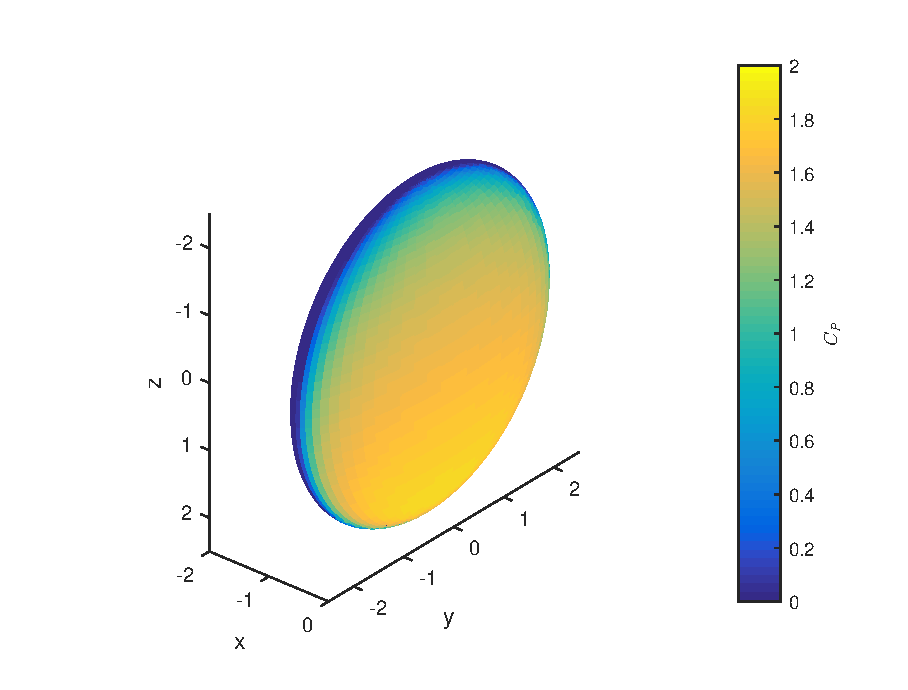
\includegraphics[angle=180, width=0.96\textwidth]{./Figure/Concepts/rigid.eps}
		\caption{Rigid concept}
		\label{fig:rigid}
	\end{subfigure}
	\begin{subfigure}[b]{0.32\textwidth}
		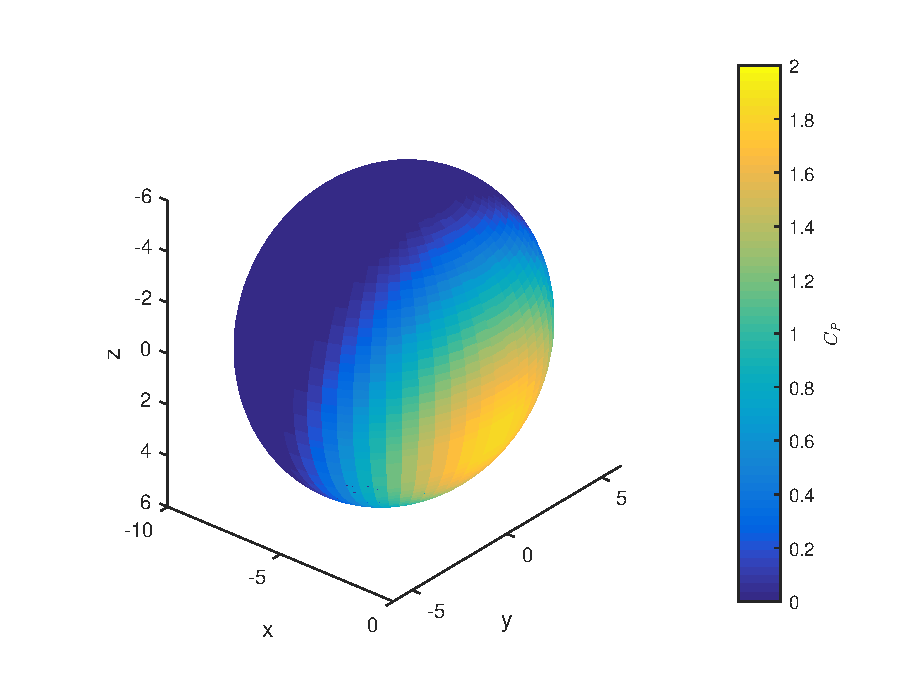
\includegraphics[width=0.96\textwidth]{./Figure/Concepts/isotensoid.eps}
		\caption{Isotensoid concept}
		\label{fig:isotensoid}
	\end{subfigure}
	\begin{subfigure}[b]{0.32\textwidth}
		\includegraphics[width=0.96\textwidth]{./Figure/Concepts/stacked_toroid.eps}
		\caption{Stacked toroid concepts}
		\label{fig:stacked_toroid}
	\end{subfigure}
	\begin{subfigure}[b]{0.32\textwidth}
		\includegraphics[width=0.96\textwidth]{./Figure/Concepts/tension_cone.eps}
		\caption{Tension cone concept}
		\label{fig:tension_cone}
	\end{subfigure}
	\begin{subfigure}[b]{0.32\textwidth}
		\includegraphics[width=0.96\textwidth]{./Figure/Concepts/trailing_ballute.eps}
		\caption{Trailing ballute concept}
		\label{fig:trailing_ballute}
	\end{subfigure}
\caption{Overview of design concepts (Courtesy of Irene Heemskerk)}
\label{fig:concepts}
\end{figure}
\section{System definition}\label{cha:sysdef}

This chapter discusses the system definition. First off the functions of the system are discussed in Section \ref{sec:funcdef}. The system is further broken down in subsystems in Section \ref{sec:subsysbreak}. Finally the technical risks of the system are discussed in Section \ref{sec:sysrisk}.


\subsection{Functional definition} \label{sec:funcdef}
The entry vehicle is required to perform the functions listed in the functional breakdown structure of Figure \ref{fig:fbs}, which categorises the main vehicle functions. These functions can subsequently be attributed to the subsystems partaking in the mission.

\begin{figure}[h]
	\includegraphics[width=0.95\textwidth]{./Figure/subsystem_breakdown/FBS.pdf}
	\caption{Entry vehicle functional breakdown structure}
	\label{fig:fbs}
\end{figure}

Sequencing the functions of the functional breakdown structure in time yields the functional flow diagram in Figure \ref{fig:ffd}. Sequencing of sub-functions 3.1-3.2, 4.0-4.5 and 5.0-5.8 is taken up in the respective sections discussing their design. Sub-functions 1.1-1.4, 2.1-1.5 and 6.1-6.3 are performed continuously.

\begin{figure}[H]
	\includegraphics[width=1.00\textwidth]{./Figure/subsystem_breakdown/FFD.pdf}
	\caption{Entry vehicle functional flow diagram}
	\label{fig:ffd}
\end{figure}





\subsection{Subsystem breakdown} \label{sec:subsysbreak}
A tally was made of all the subsystems included in the spacecraft. First a division can be made by distinguishing between the subsystems pertaining to the crew module and those included in the \gls{hiad}. This division is shown in figure \ref{fig:subsystems}. Also shown in figure \ref{fig:subsystems} are all the subsystems included in the crew module and decelerator.
\begin{figure}[h]
	\includegraphics[width=0.95\textwidth]{./Figure/subsystem_breakdown/subsystem_breakdown.pdf}
	\caption{Spacecraft subsystem breakdown}
	\label{fig:subsystems} 
\end{figure}
There exist some links between several of the subsystems. 

\subsection{Technical risks} \label{sec:sysrisk}
In order to identify which areas and components might present a risk to the technical performance of the system or cause schedule overruns a risk map is made. This risk map is presented in section \ref{subsec:riskmap} along with its elements. Following the concept-independent risk assessment section \ref{subsec:developrisk} will discuss the concept-specific development risks, based on the technology maturity of each concept. The assessment of these development risks will be used in Chapter \ref{ch:tfsum} as one of the criteria used during the trade-off process.\\

\subsection{Concept-independent risk assessment} \label{subsec:riskmap}
Before the concept-specific development risks are discussed the concept-independent risks were analysed in order to determine how to allocate the resources available for the concept selection and trade-off process. To do this the concept-independent elements are first listed in Table \ref{tab:riskmapelements}, after which they are placed inside a risk map. Each of these elements gets assigned a \acrfull{trl} \cite{NASA2007} based on the maturity of the technology that will be used in said element. The \gls{trl}-classification is shown in Table \ref{tab:trls}.\\

The concept-independent risk elements shown in Table \ref{tab:riskmapelements} have been used as input to construct the risk map, shown in Table \ref{tab:riskmap}.\\

\begin{table}[h]
	\caption[\acrfull{nasa} \acrfullpl{trl}]{\acrfull{nasa} \acrfull{trl} \cite{NASA2007}}
	\begin{tabular}{|p{0.2\textwidth}|p{0.75\textwidth}|}
		\hline
		\textbf{\acrfull{trl}} & \textbf{Description} \\ \hline \hline
		\gls{trl} 9& Actual system "flight proven" through successful mission operations\\
		\gls{trl} 8& Actual system completed and "flight qualified" through test and demonstration (ground or space)\\
		\gls{trl} 7& System prototype demonstration in a space environment\\
		\gls{trl} 6& System/subsystem model or prototype demonstration in a relevant environment (ground or space)\\
		\gls{trl} 5& Component and/or breadboard validation in relevant environment\\
		\gls{trl} 4& Component and/or breadboard validation in laboratory environment\\
		\gls{trl} 3& Analytical \& experimental critical function and/or characteristic proof-of-concept\\
		\gls{trl} 2& Technology concept and/or application formulated\\
		\gls{trl} 1& Basic principles observed \& reported \\
		\hline
	\end{tabular}
	\label{tab:trls}
\end{table}

\begin{table}[h]
	\centering
	\caption{Risk map elements}
	\label{tab:riskmapelements}
	\begin{tabular}{|c|c|}
		\hline 
		\textbf{Number} & \textbf{Element} \\ \hline \hline
		1 & \acrlong{tps}-material \\
		2 & \acrlong{tps}-conections\\
		3 & Structural materials\\
		4 & Structural conections\\
		5 & Inflation system	\\	
		6 & Deployment mechanism\\
		7 & Descellerator-capsule-joints\\
		8 & Aerodynamic shape\\
		9 & Pressure sensors\\
		10 & Bank-control thrusters\\
		11 & \gls{adcs} thrusters\\
		12 & \gls{adcs} reaction wheels\\
		\hline
	\end{tabular}
\end{table}

\begin{table}[H]
	\centering
	\caption{Risk map}
	\label{tab:riskmap}
	\begin{tabular}{|c|c|c|c|c|} % MAKE SURE THAT THE TOTAL WIDTH IS 0.95\textwidth!! (that way its exactly the textwidth.... haha) 
		\hline
		\textbf{\gls{trl} 1} & \cellcolor{green!70} & \cellcolor{yellow!75} 3, 4 & \cellcolor{red!60} & \cellcolor{red!60} 10 \\ \hline
		\textbf{\gls{trl} 2} & \cellcolor{green!70} & \cellcolor{yellow!75} 6, 9 & \cellcolor{red!60} & \cellcolor{red!60} \\ \hline
		\textbf{\gls{trl} 3} & \cellcolor{green!70} & \cellcolor{yellow!75} & \cellcolor{red!60} 8 & \cellcolor{red!60} 7, 11 \\ \hline
		\textbf{\gls{trl} 4} & \cellcolor{green!70} & \cellcolor{yellow!75} & \cellcolor{yellow!75} & \cellcolor{yellow!75} \\ \hline
		\textbf{\gls{trl} 5} & \cellcolor{green!70} & \cellcolor{green!70} & \cellcolor{yellow!75} 2 & \cellcolor{yellow!75} \\ \hline
		\textbf{\gls{trl} 6} & \cellcolor{green!70} & \cellcolor{green!70} & \cellcolor{green!70} & \cellcolor{green!70} 1, 5 \\ \hline
		\textbf{\gls{trl} 7} & \cellcolor{green!70} & \cellcolor{green!70} & \cellcolor{green!70} & \cellcolor{green!70} \\ \hline
		\textbf{\gls{trl} 8} & \cellcolor{green!70} & \cellcolor{green!70} & \cellcolor{green!70} & \cellcolor{green!70} \\ \hline
		\textbf{\gls{trl} 9} & \cellcolor{green!70} & \cellcolor{green!70} & \cellcolor{green!70} & \cellcolor{green!70} \\ \hline
		 & \textbf{Negligible} & \textbf{Marginal} & \textbf{Critical} & \textbf{Catastrophical} \\ \hline
	\end{tabular}
\end{table}






\section{Crew module design and sizing}\label{ch:crewmod}
It is essential that the crew module is designed and sized for the following purposes. Firstly, it is a prerequisite to size control mechanisms as the crew module is a dominant contributor to mass moments of inertia by its large mass. Secondly, it allows determination of the number of crew members to be taken on board and thereby to investigate advantages of an inflatable aerodynamic decelerator over the conventional rigid solution, such as Orion. Thirdly and most importantly, it is required to yield a full mission description.

To this end, crew module subsystems are designed and sized at a preliminary design level in section \ref{sec:crewsubsys}. Each subsystem is given and and accompanied by mass, power and volume budgets. The latter two allow for packaging of the crew module to effect a \gls{cg} location that minimizes required control system activity. Crew module subsystem integration is described in section \ref{sec:crewpackaging}. The crew module configuration is carried through in the final design as an input for the control system as well as to harmonize a design that integrates crew module and decelerator.

\subsection{Subsystem design and sizing} \label{sec:crewsubsys}
The \acrfull{adcs}, \acrfull{cdh}, operational items (including life support), capsule structure, thermal control and power and the terminal descent system are key components of the crew module. A basic sizing and design follows hereafter.

\subsubsection{Attitude determination and control} \label{subsec:adcs}
The general objectives for the \gls{adcs} is to monitor the attitude of the spacecraft and perform corrections if needed. The operation period of the \gls{adcs} can be divided into two phases, the interplanetary phase and the Mars approach phase.

During the interplanetary flight the \gls{adcs} keeps the attitude as required to point the solar arrays toward the sun, point the thrusters in the desired direction etc.

During the Mars approach phase the \gls{adcs} should adjust the attitude to the entry attitude, and compensate for possible disturbances (i.e. inflation of the \gls{hiad})

\paragraph{Sensors} Sensors are needed to determine the attitude. How accurate the sensors need to be depends on the required accuracy from different subsystems, for instance a high gain antenna requires a higher accuracy. 

\subparagraph{Star trackers}
Star trackers work by taking pictures of the stars and comparing them to an internal catalogue. They are the most accurate for pointing \cite{CarlChristianLiebe1995}. However they do not work if the spacecraft is rotating to fast, so an additional rough estimate is needed \cite[p. 584]{Wertz2011}. 

The mass of star trackers is in the order of a 100 $\left[g\right]$. The required operating temperature range is -30 $\left[^\circ C\right]$ to +50 $\left[^\circ C\right]$. The average power consumption is 0.5 $\left[W\right]$.\footnote{\label{ftn:star_tracker}http://www.sinclairinterplanetary.com/startrackers Accessed: 11-06-2015}

\subparagraph{Gyroscope}
Gyroscopes can be used to provide the attitude determination for the initial stabilization. There are different kinds of gyroscopes, mechanical, optical and the so called \gls{mems}. The latter one is relatively new, and is widely used in mobile phones. 

\subsubsection{Command, data handling and telemetry} \label{subsec:cdh}
\acrfull{cdh} and telecommunications form an integral part of the avionics system. These perform four functions: flight and vehicle control, data processing, human interfacing and communications \cite{Eger2008}. This requires adirect links to the \gls{adcs} module, a link to the telecommunications network and a link to on-board display for crew members. These are illustrated in Figure \ref{fig:cdhflow}

\begin{figure}[h]
		\centering
		\includegraphics[width=1.0\textwidth]{./Figure/CrewModule/CDH.pdf}
		\vspace{-12mm}
		\caption{Communication flow}
		\label{fig:cdhflow}
\end{figure}

Data processing is performed as follows. Data is firstly filtered, then analyzed to see if reactions are required and in case reactions are required put through to the relevant effectors (subsystems) and critical system information communicated to the ground station via the Ka-band (see section \ref{sec:groundop}). Modulation is performed in the transponder by \gls{bpsk} on carrier and subcarrier (modulating the carrier) and \gls{qpsk} on the carrier, similar to the Mars Reconnaissance Orbiter mission \cite{Taylor2006}.

For its integral part, it is key that the system is redundantly equipped to ensure adequate system reliability. To this end, cabling is redundant and safety-critical processing tasks are performed by self-checking pair processors, following their application in Orion \cite{Eger2008}. These self-checking pair processors observe and compare the activity of their partner to identify faulty behavior. 

Antennas used can be extracted from a reference mission to Mars, for example the Mars Reconnaissance Orbiter \cite{Taylor2006}. This mission had relatively high scientific return communications and used a 3 [$m$] diameter high gain antenna and two low gain antennas. The communication system for this mission was remarkable because it was able to send data back to Earth more than ten times faster than previously conducted missions. Such a high return would be highly beneficial for the manned mission at hand to maximize ground surveyance possibilities and accurate monitoring. It similarly used Ka-band communication for downlink. To this end, the communication system is deemed a good reference system for use in the mission at hand.

The mass of the \gls{cdh} subsystem is extrapolated from that in the Mars Odyssey mission by scaling with the ratio of masses. For a 11.1 [$kg$] \gls{cdh} subsystem mass in the 376 [$kg$] Mars Odyssey\footnote{URL:\url{http://mars.nasa.gov/odyssey/mission/spacecraft/parts/command/}. Accessed: 11-06-2015}, this translates to nearly 300 [$kg$] on the 10 000 [$kg$] entry vehicle at hand. This telecommunications system had a mass of 108 [$kg$], which is not scaled since the sizing thereof is not deemed mass-dependent. Taking into account a contingency for the larger crew module and more demanding mission at hand as well as the roughness of the estimates, the \gls{cdh} and telecommunications mass is estimated at 530 [$kg$], thus taking a 30 $\%$ contingency into account. In addition, cabling requires additional contingency, taken to be 10 $\%$ and a mass of 53 [$kg$].


\subsubsection{Operational items} \label{subsec:crewop}
In this section the operational items are sized. This can be summarised as the mass needed by the astronauts to live under reasonably comfortable conditions in the crew module during the mission. For this purpose the paper by Tito et al has been used \cite{Tito2013}. In this paper the operational items are called \acrfull{eclss}. First the method for estimation is described with its assumptions. Followed by the results of the estimation.

\paragraph{Estimation method}
The mass of the \gls{eclss} is primarily driven by the crew size and mission length. The \gls{eclss} is divided into subsystems: Air Management, Thermal and Humidity Management, Water Management, Waste Management, Human Accommodation, Food Preparation and Storage. Each of these subsystems can be subdivided into components. Examples of these are a water heater or packed food in the Food Preparation and Storage. It is evident that some components scale with the keydrivers and others do not. For example, adding a crew member does not necessitate an extra water heater, but it does require extra packed food. 


Taking this into account the mass has been divided into two components. A basic system mass which scales with crew size and the consumable mass that scales with crew size and mission length. Examples of components that belong to the basic system mass are oxygen scrubbers (not including oxygen), atmospheric control systems and food preparation systems. Examples of components that belong to consumable mass are oxygen, food, water and personal provisions. The used reference by Tito et al incorporates the mass for the \gls{tcs}. It is assumed that this \gls{tcs}-mass only provides the thermal control for the operational items. The \gls{tcs} for other subsystems is discussed in Section \ref{subsec:crewthermalcontrol}.

\paragraph{Results}
By using the method described in the previous paragraph the results of Table \ref{tab:operationalest} were obtained.
\begin{table}[h]
	\centering
	\caption{Obtained masses and volumes of basic system \& consumable items}
	\begin{tabular}{|p{1.9cm}|p{2.7cm}|p{2.7cm}|p{3.5cm}|p{3.6cm}|}
		\hline
		\textbf{Crew members} & \textbf{Basic system mass $[kg]$} & \textbf{Basic system volume $[m^{3}]$} & \textbf{Consumables mass per day $[kg]$} & \textbf{Consumables volume per day $[m^{3}]$} \\ \hline \hline
		1 & 1,800 & 4.88 & 3.2 & 0.018 \\
		2 & 2,500 & 6.78 & 6.4 & 0.036 \\
		3 & 3,200 & 8.68 & 9.6 & 0.054 \\
		\hline
	\end{tabular}
	\label{tab:operationalest}
\end{table}
It can be seen from Table \ref{tab:operationalest} that both the basic system and consumables mass scale with the number of crew members. By using linear extrapolation the mass and volume associated with crew members higher than three can be determined. These are shown in Table \ref{tab:crewmemberops} for a mission time of $100$ days, which incorporates the transfer from Earth to Mars and the maximum deceleration time. Herein the \gls{tcs}-mass for the operational items comes down to 480 $[kg]$.\\

\begin{table}[h!]
	\caption{Total mass and volume associated with operational items for varying crew numbers}
	\begin{tabular}{|c|c|c|}
		\hline
		\textbf{Crew members} & \textbf{Operational items mass $[kg]$} & \textbf{Operational items volume $[m^{3}]$}\\ \hline \hline
		1 & 2,120 & 6.69\\
		2 & 3,140 & 10.40\\
		3 & 4,160 & 14.11\\
		4 & 5,180 & 17.82\\
		5 & 6,200 & 21.53\\
		6 & 7,220 & 25.24\\ \hline
	\end{tabular}
	\label{tab:crewmemberops}
\end{table}
Furthermore Rudisill et al mention the spacecraft volume required for crew operations per crew member \cite{Rudisill2008}. This volume can take on three different values depending on the mission length. The resultant habitable volumes are shown in figure \ref{fig:crewvolume}.
\begin{figure}[h]
	\centering
	\includegraphics[scale=1.0]{./Figure/CrewModule/Crewvolume}
	\caption{Habitable volume per crew member as a function of mission duration \cite{Rudisill2008}}
	\label{fig:crewvolume}
\end{figure}
In the remainder of this report the crew habitable volume will be sized to the 'performance limit' indicated in figure \ref{fig:crewvolume}.


\subsubsection{Capsule structure} \label{subsec:crewstruc}
The structure of the crew module serves the important function of connection all the individual subsystems of the crew module and moreover connects with the \gls{cia}. The main scope of the design described in this report lies within this \gls{cia}. New advances from for example the currently being developed and Orion mission are therefore not considered. The Orion capsule can already be considered state of the art and is in a large amount representative for the crew module design.

A schematic layout as for example also used in the Orion spacecraft\footnote{URL: \url{http://www.spaceflight101.com/orion-spacecraft-overview.html}, Accessed 11 June 2015 }, features a Aluminium grid structure. This structure encloses the pressurised volume inhabited by the astronauts. The grid structure allows for easy attachment of the individual subsystems. Subsystems which require pressurisation, typically those involving the astronauts can be placed within in this shell, whereas the systems that do not require pressurisation are placed on the outside of this shell. A more detailed analysis on where each of these individual subsystems are placed is discussed in Section \ref{sec:crewpackaging}.


A full estimate of the structural mass is only to be provided in later design phases. More detailed structural estimates are typically provided by detailed \gls{cad} models and \gls{fem} models \cite{Wertz2011}. A rough estimate can be provided on the basis of previous reference missions. \gls{nasa}'s Orion mission is again of primary interest as it also features astronauts. Some differences with respect to the structural elements thereof can however be noted:

\begin{itemize}
\item Orion incorporates an integrated heat shield and structure
\item Orion features a backshell, not required for the inflatable aeroshell by its larger deployed diameter
\end{itemize}

In the design at hand the heat shield structure is incorporated in the \gls{cia}. The crew module is merely connected to this \gls{cia} of which the latter is designed in more detail in the remaining chapters of this report. Due to the implementations of the \gls{cia} an additional backshell structure is also no longer required. The back shell normally functions a protection against thermal loading which moves sideways along the body. Using the large frontal of the inflatable this is prevented, denoting one of the advantages of using a inflatable structure \cite{Hughes2005}. The crew module structure should however also be sized considering , and may as such not be too tall and may feature a tapered end such that the crew module is not exposed to thermal loading passing the \gls{cia}.

For this reason the heat shield carrier structure of around $1500 \left[kg\right]$ \cite{Ainsworth2014} is not taken into account into the mass estimate of the structure. A total structural mass for manned re-entry vehicles lies at around 30\%. The manned Apollo mission featured a 31\% structural mass fraction \footnote{URL: \url{http://braeunig.us/space/specs/apollo.htm}, Accessed 11 June 2015} including a heat shield structure. Extrapolating this value, with a $9000 \left[kg\right]$ crew module mass yields a structural mass of $1300 \left[kg\right]$, excluding the heat shield structure. This is in line with values suggested by Wertz et al. \cite{Wertz2011}. Taking into account a 30\% mass contingency factor yields a final structural mass estimate of around $1700 \left[kg\right]$. A similar mission featuring a descent towards Mars from $7 \left[km \cdot s^{-1}\right]$ has a structural mass of $517 \left[kg\right]$ on a dry mass of $2863 \left[kg\right]$ including contingency factors\footnote{URL: \url{http://www.nasa.gov/pdf/458812main\_FTD\_AerocaptureEntryDescentAndLanding.pdf} , Accessed 11 June 2015 }. Scaling this value yields a similar mass estimate of around $1800 \left[kg\right]$. 

The connection between the crew module and the \gls{cia} is taken into account in the capsule structural mass estimate of $1300 \left[kg\right]$.

\subsubsection{Capsule thermal control} \label{subsec:crewthermalcontrol}
Where the \acrfull{tps} is used to protect the crew module from excessive heating during re-entry, the \acrfull{tcs} is used to keep other subsystems in the crew module within their operating temperature limits. It is assumed that re-entry phase does not impose extra requirements on the \gls{tcs} as it is completely covered by the \gls{tps}. Note that this only holds when the angle of attack ($\alpha$) is low enough such that the crew module stays out of the wake. Furthermore, the paper by Tito used in the mass estimation for the operational items already assigns a mass for the thermal control within the living compartments of the crew module \cite{Tito2013}. The paper calculates a mass of 480 $[kg]$ for a crew module suitable for the life support of two astronauts. Therefore this part only focuses on the thermal control of components that are not placed within the living compartments.

Examples of these components that need to operate at the edge or outside of the crew module are star trackers from the \gls{adcs} or the antennas from the telecommunications. To provide typical temperature limits, Table 22-9 \textcolor{red}{from SMAD} is provided in Table \ref{tab:cmtherm} \cite{Wertz2011}. In here there is a distinction between operational and surviving temperatures. From this table it is evident that components that operate outside the spacecraft can typically handle a wider temperature range than components that operate within the crew module.

\begin{table}[h]
	\centering
	\caption{Typical temperature requirements for different components}
	\begin{tabular}{|l||l|l|}
		\hline
		\textbf{Equipment} & \textbf{Operational range $\mathbf{[^{\circ}C]}$} & \textbf{Survival range $\mathbf{[^{\circ}C]}$}\\ \hline \hline
		Avionics Baseplates & -20 $-$ 60 & -40 $-$ 75 \\
		Batteries & 10 $-$ 30 & 0 $-$ 40 \\
		Hydrazine Fuel & 15 $-$ 40 & 5 $-$ 50 \\
		Solar Arrays & -150 $-$ 110 & -200 $-$ 130 \\
		Antennas & -100 $-$ 100 & -120 $-$ 120 \\
		Reaction Wheels & -10 $-$ 40 & -20 $-$ 50 \\
		\hline
	\end{tabular}
	\label{tab:cmtherm}
\end{table}

In order to keep the subsystems within their operative temperature range the \gls{tcs} uses different tools and techniques. According to Karam the most commonly used are coatings, insulators and isolators, heaters, louvers and heat pipes \cite{Karam1998}. For this stage of design of the crew module it is deemed sufficient to only provide a mass estimate for the \gls{tcs}-mass.

\textcolor{red}{According to SMAD} the \gls{tcs}-mass ranges from 3\% to 10\% with an average of 6\% for the dry mass of a interplanetary spacecraft \cite{Wertz2011}. Note that these spacecraft are not aimed to carry astronauts, therefore it is assumed that this 6\% adds on top of the 480 $[kg]$ calculated in Section \ref{subsec:crewop}. This would add an extra 600 $[kg]$ dedicated to the \gls{tcs}.


\subsubsection{Capsule power} \label{subsec:pwer}
Small introduction on the purpose of the power subsystem.\\

Piece on the items that the power subsystem needs to drive.\\

Small trade-off / considering possible options for power generation. (solar arrays, batteries, reactor)\\

conclusion on mass and volume.\\





\subsubsection{Terminal descent system} \label{subsec:crewtermdescent}
Terminal descent takes place in the following sequence, depicted schematically in Figure \ref{fig:tdseq}.
\begin{enumerate}
\item The rigid heat shield, joined in the middle by a bolt-and-nut assembly, is separated by redundant pyrotechnic cutters. The two halves are held fixed by locking actuators to prevent interference with exhaust flow and inflatable.
\item At this altitude, retropropulsion is activated and the thruster provides the decelerating force in combination with the inflated aeroshell.
\item At an altitude of 50 [$m$], struts are partially deployed from their stowed position such that the pads rest above the inflatable. At the same time, the vent in the inflation system is opened and inflatable bladders deflate. Upon full deflation, measured by pressure transducers in the inflation system, the struts deploy further such that the pads are level with but below the thruster nozzle exit and achieve a roughly 90 [$deg$] inflatable half-cone angle.
\item The thruster is then deactivated and the crew capsule lands on the inflatable, on which the landing gear pads rest.
\end{enumerate}
\begin{figure}[h]
	\centering
	\begin{subfigure}[b]{0.44\textwidth}
		\includegraphics[width=0.96\textwidth]{./Figure/CrewModule/TDa.pdf}
		\caption{Retropropulsion activation}
		\label{fig:rot}
	\end{subfigure}
	\begin{subfigure}[b]{0.54\textwidth}
		\includegraphics[width=0.96\textwidth]{./Figure/CrewModule/TDb.pdf}
		\vspace{-4.5mm}
		\caption{Decelerator deflation}
		\label{fig:fold}
	\end{subfigure}
		\begin{subfigure}[b]{0.55\textwidth}
		\centering
			\includegraphics[width=0.96\textwidth]{./Figure/CrewModule/TDc.pdf}
			\caption{Strut deployment}
			\label{fig:hinge}
		\end{subfigure}
	\caption{Terminal descent activity sequence}
	\label{fig:tdseq}
\end{figure}


Retropropulsion is used for the beneficial aerodynamic interaction with a \gls{hiad} \cite{xxx}, effecting a required specific impulse that is twice as low as otherwise. This effects a smaller propellant mass required. The inflatable is not rejected, but rather deflated, because rejection would require a separation mechanism to prevent interference with the crew capsule. Deflation does induce, however, the risk that it is not performed reliably. In such a case, a risk mitigation plan could be deliberate puncturing of the inflatable bladder volumes in order to deflate it.

[THRUSTER MASS]


The terminal descent system, as described in Section \ref{sec:terminal}, consists of the thruster system that decelerates the spacecraft from Mach 5 at 10 [km] height to zero velocity at a height of 0 [km]. The thruster should be placed in the centerbody and pointed in the forward direction, such that the positive interaction between aerodynamics and the thruster plume is made use of. The total thruster mass, including fuel is estimated to be approximately 1300 [kg], based on extrapolation of .................
The thruster mass is estimated to be 470 [kg], based on a 3g deceleration and using an empirical relation\cite{Christian2006}. This leaves approximately 930 [kg] for the fuel. Assuming the density of the fuel at 1000 $[kg\cdot m^{-3}]$\footnote{\url{http://en.wikipedia.org/wiki/Liquid-propellant_rocket}. Accessed: 11-06-2015} means the required volume for fuel is 0.93 [$m^3$].






\subsection{Crew module configuration} \label{sec:crewpackaging}
Space allocation of the subsystems described in the previous section, as well as crew members, is performed with the goals of:
\begin{itemize}
\item Accommodating subsystems necessary to support interplanetary flight and entry
\item Providing crew members with a habitable volume and operational items to support a flight duration of approximately 100 days
\item Keeping the axial position of the \gls{cg} forward to lower pitch stability and alleviate pitch control performance in the final mission phase
\item Allowing for packaging freedom in achieving a static lateral \gls{cg}-offset for creating an asymmetric lifting shape
\end{itemize}
To this end, the crew module is packaged as depicted in Figures \ref{fig:axview}, \ref{fig:axview2} and \ref{fig:topview}. 

The top part is required to contain drogues to stabilise the entry vehicle in its final descent phase. Four drogues are placed to incorporate redundancy and provide a symmetric configuration, to prevent excessive tilting during final descent. Moreover, the top part contains the foldable solar arrays required to generate power required during interplanetary transfer. These are placed in the top part to prevent interference with firstly the exhaust flow from thrusters and secondly the stowed inflatable before entry on the other hand. A high-gain antenna of adjustable attitude on a boom enables communication during all mission phases. Thrusters for the apoaerion boost are mounted on top, of 0.41 $[m]$ length. Therefore the length of the top part is estimated on the basis hereof to be 0.50 $[m]$ length.

Crew members are located in the next part, a habitable volume to their availability that is dictated by the performance limit for a three-month mission duration as 11 $[m^{3}]$ per crew member \cite{Rudisill2008}. The diameter of the habitable volume is 4.0 $[m]$, thereby less than vehicle maximum diameter to accommodate four propellant tanks, one per quadrant. Propellant tanks allow intertank propellant transfer to maintain the lateral \gls{cg} position. The tanks are sized on the basis of the total required propellant and provide propellant for both the reaction control thrusters, apoaerion boosters and retro-propulsion thruster assembly. The length of this part follows from the habitable volume and depends on the number of crew members. For two crew members, it is 1.75 $[m]$ long. Including a 0.25 $[m]$ contingency for an aft pressure bulkhead yields an estimated length of 2.00 $[m]$.

Operational items are located within reach of crew members. These are placed at this location because of their relatively high mass and therefore contribution to the axial \gls{cg} position. The total volume occupied follows from Table \ref{tab:crewmemberops}. On one hand these operational items include relatively dense products, foremostly the life support systems, and less dense products in the form of food and other supplies.  The length of this part follows from the required volume for operational items, for two crew members equal to 0.75 $[m]$. Including a forward additional bulkhead yields an estimated length of 1.00 $[m]$.

%Arranging these items asymmetrically allows for a lateral \gls{cg}-offset, most notably considering the depleted supplies of food at the end of interplanetary transfer while life support system mass remains intact.

Four struts for touchdown, packed symmetrically. The struts are arranged about the batteries required to provide power during entry, when solar panels are stowed, and the main thrusters for retro-propulsion. The length follows from estimates for the strut required volume and the retro-propulsion thrusters of 2.30 $[m]$ length. It is an estimated 2.0 $[m]$, as part of the thruster is contained within the last part.

The last part contains the thruster nozzle, closed off by a heat-resistant end-cap during entry, a nitrogen tank and inflation system, and the attachment rings for the inflatable decelerator. The end-cap is to be eject-able. The length of this part is mainly dictated by the shape of the inflatable and where it attaches to the centre body. For a 12.0 $[m]$ deployed diameter, it is approximately 1.0 [$m$] in length.

This yields a total vehicle length of an estimated 6.5 $[m]$. This fits within \gls{sls} fairing constraints  and moreover ensures that the crew module is not impinged by the flow.

\begin{figure}[h]
		\centering
		\includegraphics[width=0.95\textwidth]{./Figure/CrewModule/Axialview.pdf}
		\caption[First axial view of crew module lay-out]{First axial view of crew module lay-out. Space allocation only, drawing not to scale.}
		\label{fig:axview}
\end{figure}

\begin{figure}[h]
		\centering
		\includegraphics[width=0.95\textwidth]{./Figure/CrewModule/Axialview2.pdf}
		\caption[Second axial view of crew module lay-out]{Second axial view of crew module lay-out. Space allocation only, drawing not to scale.}
		\label{fig:axview2}
\end{figure}

\begin{figure}[h]
		\centering
		\includegraphics[width=0.95\textwidth]{./Figure/CrewModule/TopviewV2.pdf}
		\caption[Top-down view of crew module lay-out]{Top-down view of crew module lay-out. Space allocation only, drawing not to scale.}
		\label{fig:topview}
\end{figure}

Component masses are as listed in Table \ref{tab:crewmass}. Due to the relative large mass of items closer to the aeroshell the axial \gls{cg} position is estimated closer than 3 $[m]$ from the inflatable aeroshell attachment point. A more elaborate estimate is without value, for the actual packaging of the crew module requires a more thorough design beyond the mission scope. However, to investigate the feasibility of achieving the required \gls{cg}-offset, it follows from Figure \ref{fig:cgoffset} that the required \gls{cg}-offset is below 0.5 $[m]$. Such an offset can be affected primarily by shifting the relatively heavy contributions of operational items. Placing the \gls{cg} thereof 1.5 $[m]$ from the axial centreline and assuming a symmetric configuration otherwise yields an approximate 0.5 $[m]$ lateral \gls{cg}-offset. Considering the 4.5 $[m]$ diameter allocated to operational items, this is feasible. %In addition, pumping fuel from tank to tank provides a measure of \gls{cg} position control.

\begin{table}[h]
\centering
\caption{Crew module mass budget}
\label{tab:crewmass}
\begin{tabular}{|l|c|}
\hline
{\bf Component}    & {\bf Component mass {[}kg{]}} \\ \hline \hline
Power              & 280                           \\ \hline
 ADCS        &  225                     \\ \hline
Thermal            & 600                           \\ \hline
Structural mass    & 1300                          \\ \hline
Operational items  & 3140                          \\ \hline
Crew               & 160                           \\ \hline
Terminal descent   & 1445                          \\ \hline
C\&DH              & 585                           \\ \hline 
Other    & 815                          \\ \hline \hline
\textbf{Total}    & \textbf{8550}                          \\ \hline \hline
Margin ($5\%$)  & 450                        \\ \hline \hline
{\bf Capsule mass} & {\bf 9000}                    \\ \hline
\end{tabular}
\end{table}





\section{Design parameters and tool analysis}\label{cha:designpar}
It is essential for the iterative design process that the design sensitivity is investigated. This sensitivity is quantified by tools for trajectory, thermal structural and aerodynamic analysis. These tools are complemented by a control system tool for the purpose of control system design and sizing. The description of these tools is given in Section \ref{sec:designtools} and their output in Section \ref{sec:designsens}.

\subsection{Design tools} \label{sec:designtools}
Subsequent Sections describe the trajectory, aerodynamic, control, thermal and structural analysis tools. A brief overview of the underlying principles, assumptions and in- and output is given.
\subsubsection{Trajectory analysis}\label{subsec:orbittool}
\subsubsection{Discretisation error}
\label{sec:astrodisc}

Due to the use of a discrete time step an error relative to the real solution is induced. By testing the tool with the same initial conditions using different time meshes the difference between the solutions can be analysed. When the smallest time step is assumed to be exact, the error of the larger time steps can be expressed relative to that. This relative error is shown in Figure \ref{fig:atmos_disc}. Please also note these errors are calculated running the tool without active control.

Two conclusions can be drawn from this. First the error decreases quadratically with decreasing time step. This means that the system converges. Secondly the error is smaller than 1 $\left[m\right]$ for a time step smaller than $0.3$ $\left[s\right]$. This error is negligible compared to the error that will be induced by the assumptions that were made in Section \ref{sec:astroassumption}.

%Initial Position
%rx = -4143775;
%ry = 10*R_m;
%R = [rx,ry,0];

%Initial Velocity
%v = 7.1679e+03; %[m/s]
%V = [0,-v,0];

\begin{figure}[ht]
	\centering
	\includegraphics[width=0.8\textwidth]{Figure/orbit/dicretization.pdf}
	\caption[Discretisation error in location $\left(\gls{sym:Rv}\right)$ after one pass through the atmosphere for the rigid shape]{Discretisation error in radius $\left(\gls{sym:Rv}\right)$ after one pass through the atmosphere for initial position $\left[-4$ $143$ $775,10\cdot\gls{con:rm}\right]$ $\left[m\right]$ and initial velocity $\left[0,-7167.9\right]$ $\left[m\cdot s^{-1} \right]$ at $\gls{sym:alpha}=-10$ $\left[deg\right]$ for the rigid shape}
	\label{fig:atmos_disc}
\end{figure}

\subsubsection{Verification through comparison with Kepler orbit}
\label{sec:astroverf}

In this section the results from the numerical simulation, which is usually only used in atmosphere, is compared to a Kepler orbit. For this comparison the density is assumed to be zero, or in other words, it is assumed that there is no atmosphere. This comparison is done for different values of $\Delta t$. The error for each $\Delta t$ is shown in Figure \ref{fig:kep_error}.

\begin{figure}[ht]
	\centering
	\includegraphics[width=0.8\textwidth]{Figure/orbit/num_kep.pdf}
	\caption[Error compared to a Kepler orbit]{Error compared to a Kepler orbit after 50 005 seconds for initial position $\left[-4$ $143$ $775,10\cdot\gls{con:rm}\right]$ $\left[m\right]$ and initial velocity $\left[0,-7167.9\right]$ $\left[m\cdot s^{-1} \right]$ at $\gls{sym:alpha}=-10$ $\left[deg\right]$ for the shape of the rigid concept}
	\label{fig:kep_error}
\end{figure}

The figure shows the error is between 15 and 5 for $\Delta t$ between 1 and 0.01. The error decreases, but seems to tend to a non-zero constant value. The method used for numerical simulation is thus convergent, but has a small offset from the exact solution. This error is however so small it can easily be accepted. It should also be noted that the numerical simulation is never ran longer than 2000 seconds during the entire mission trajectory calculation. The error calculated here is thus much larger than the error in the actual calculations will be.

\subsubsection{Validation}
\label{sec:astroval}

Validation for a mission as unique as this one is difficult as no reference data is available. Testing is thus the only method to do any validation of the model. Because of budget and time constraints of the conceptual design, testing is not possible. Engineering gut feeling is now the only way to get an idea of the correctness of the model. No final conclusions can be drawn from this, and thus no conclusion will be drawn.

\subsubsection{Aerodynamic analysis}\label{subsec:aerotool}
This section will investigate the influence of the shape of the re-entry vehicle on several important design parameters, as well as the sensitivity of these parameters to changes in vehicle shape. It will start by identifying the most important design parameters. This will be followed by a section discussing which shapes will generate a local optimum for a single design parameter. The knowledge of these single parameter optima will be used in the final section to discuss the total set of design parameters for various vehicle shapes. 

\paragraph{Important parameters}
This section will identify the important parameters that depend on the shape of the vehicle and will explain their significance. The following factors were determined to have a significant influence on te performance of the vehicle.

\begin{itemize}
	\item{Lift. As detailed in section \ref{subsec:controlsens}!!CHECK REFERENCE!!, the vehicle requires a lift vector to provide flight path control. A larger lift vector provides an increase in flight path control.}
	\item{Drag. The vehicle decelerates purely on atmospheric drag. An increase in drag will decrease the required time for re-entry and provides greater flexibility in terms of the path through the atmosphere. }
	\item{Lift to Drag ratio. The lift to drag ratio of the vehicle is}
\end{itemize}

\paragraph{Single parameter optima}


\paragraph{Various shapes}



\subsubsection{Control system analysis}\label{subsec:controltool}
In this section the methods used for determining appropriate control systems are explained. These systems should be able to keep the spacecraft on the trajectory as defined by the astrodynamics tool in section \ref{subsec:orbittool}. First the assumptions used and their effects on the accuracy of the analysis are explained. Than a point is determined

\paragraph{Assumptions}

**Primary and Secondary assumptions**

\paragraph{Trim point}

**Moment equilibrium figures/equations**
**CG-location plot(s)  with conclusion on CG for AoA~20 and sideslip angle=0**

\paragraph{Stability}

**From E.Mooij**

\paragraph{Available control systems}

**Intro**

\subparagraph{\acrfull{cg} offset}

**Not nessesary for AoA, not feasible for sideslip**

\subparagraph{Thrusters}

**Sebstiaan**

\subparagraph{Aerodynamic surfaces}

**Guido**





\subsubsection{Thermal analysis}\label{subsec:thermaltool}
To investigate the influence of certain design parameters on the \gls{tps} a sensitivity analysis is performed. First different materials are tested using multiple lay-ups. The different lay-ups are then used to test the influence of heat flux variations on aere density. Lastly, the variations in mass due to changing radii is investigated. This investigation is done by using the tool described in Section \ref{subsec:thermaltool}.

\paragraph{\gls{tps} materials}
Table \ref{tab:tpsmatprop} shows some promising materials that can be used in the inflatable heat shield \cite{Corso2009,Corso2011,DuPont2011,Smith2011}. These materials have been proposed during the design of multiple inflatable decelerator concepts. For each material the thermal conductivity, the density, the specific heat, the maximum operative temperature and if applicable, the emissivity are given. The latter is only applicable to the top  thermal protection layers, because these layers will radiate heat into the surroundings.

\begin{table}[H]
	\caption {flexible \acrfull{tps} material properties}
	\centering
	\begin{tabular}{|l|l|l|l|l|l|l|}
		\hline
		\textbf{Material}         & \textbf{ $\mathbf{k}$ $\mathbf{\left[\frac{W}{m\cdot K}\right]} $} & \textbf{ $\mathbf{ \rho }$ $\mathbf{ \left[ \frac{kg}{m^3} \right] }$} & \textbf{  $\mathbf{ c_{p} }$ $\mathbf{ \left[ \frac{J}{kg \cdot K} \right] }$ }& \textbf{ $\mathbf{ T_{max} }$ $\mathbf{ [ K ] }$} &\textbf{ $\mathbf{ \varepsilon }$ $\mathbf{ [ - ] }$} & \textbf{Function} \\[1.6ex]   \hline \hline
		Viton       & 0.202 & 1,842 & 1,654 & N/A	 & 0.85 & radiation coating
		\\ \hline
		Nextel AF14       & 0.150                                                 & 858                                        & 1,050                                            & 1,373	 & 0.443    & rad. and heat barrier                                 \\ \hline
		Nextel BF20       & 0.146 
		& 1,362                                        & 1,130 
		& 1,643	 & 0.443  & rad. and heat barrier                                  
		\\ \hline
		Nextel XN513      & 0.148                                                 & 1,151                                       & 1,090                                            & 1,673	 & 0.443           & rad. and heat barrier                               \\ \hline
		Refrasil C1554-48 & 0.865                                                 & 924                                        & 1,172                                            & 1,533	 & 0.7     & rad. and heat barrier                                       \\ \hline
		Refrasil UC100-28 & 0.865                                                 & 890                                        & 1,172                                            & 1,255  & 0.2       & rad. and heat barrier                                    \\ \hline
		Hexcel 282 Carbon & 0.5                                                   & 891                                        & 1,000                                            & N/A 	 & 0.9      & rad. and heat barrier                                     \\ \hline
		Pyrogel 6650      & 0.030                                                 & 110                                        & 1,046                                            & 923    & ~        & insulator                                  \\ \hline
		Pyrogel 5401      & 0.0248                                                & 170                                        & 1,046                                            & N/A  	 & ~          & insulator                                 \\ \hline
		Refrasil 1800      & 0.085                                                 & 156                                        & 1,172                                            & 1,255 	 & ~           & insulator                                \\ \hline
		Refrasil 2000      & 0.095                                                 & 180                                        & 1,172                                            & 1,366 	 & ~            & insulator                               \\ \hline
		KFA 5             & 0.25                                                  & 98                                         & 1,250                                            & 1,473 	 & ~        & insulator                                   \\ \hline
		Nomex             & 0.035                                                  & 384                                         & 1,465                                            & N/A 	 & ~        & insulator                                   \\ \hline
		Kapton            & 0.12                                                  & 1,468                                       & 1,022                                            & 673	 & ~            & gas barrier                              \\ \hline
		Upilex            & 0.29                                                  & 1,470                                       & 1,130                                            & 773 	 & ~             & structural                            \\ \hline
		Kevlar            & 0.04 & 1,440                                       & 1,420                                            & 443 	 & ~             & structural                            \\ \hline
		Vectran            & 0.37 & 1,400 & 1,259 & N/A 	 &  & structural                            \\ \hline
	\end{tabular}
	\label{tab:tpsmatprop}
\end{table}

Using the same reference a selection can be made for the most promising thermal protection and insulation layers. These are Nextel BF-20 and Nicalon for the thermal protection layers. For the insulation layers these are Pyrogel 3350 and Pyrogel 6650. Using this three lay-ups are constructed in Figure \ref{fig:layersensthermal} that are tested for different heat fluxes and radii.


\begin{figure}[h]
	\centering
	\includegraphics{./Figure/Thermal/layersensthermal.pdf}
	\caption{Tested lay-ups for the sensitivity analysis}
	\label{fig:layersensthermal}
\end{figure}

\paragraph{Effect of heat flux}
To test the effect of varying heat flux, the heat flux of an arbitrary trajectory have been multiplied to find relative values. The trajectory is found using a diameter of 12 $[m]$ and the relative factors are 0.25, 0.5, 0.75, 0.9, 1.0, 1.1, 1.4, 1.5, 2.0, 2.5 and 3.0. 

\textcolor{red}{EXTRA TEXT EN PLOTS}

\paragraph{Effect of radius}
The three lay-ups have also been tested for different radii. The aerodynamic analysis has provided heat fluxes for diameters of 6, 9, 12, 15 and 18 $[m]$. Optimising the thickness of the lay-ups for these heat flux result in Figure XX. 

\textcolor{red}{EXTRA TEXT EN PLOTS}


\subsubsection{Structural analysis}\label{subsec:structool}
Structural assessment of the inflatable configuration has been performed by an estimation of internal forces. This is an essential step in the design of an inflatable aeroshell, since it:
\begin{itemize}
%\item Is required to estimate the inflation pressure to maintain its structural integrity and aerodynamic shape under peak aerodynamic loading
\item Allows to identify whether loads allow for concept structural design within state-of-the-art material capabilities
\item Yields the loads at the structural interface between the inflatable aeroshell and the rigid centre body
\item Gives an impression of the effect of changing design parameters on concept structural performance
\item Gives insight in the structural behaviour and interaction of the inflatable
\end{itemize}
Forces are estimated for an inflatable structure that is aerodynamically loaded, as follows from vehicle trajectory analysis in its deployed condition. An interface with the aerodynamic analysis yields the optimised aeroshell shape as a baseline for the structural model used. 

Moreover, it is essential that mass contributions of centre body, inflatable structure and connections are estimated in order to verify that decelerator mass is below the 1000 [kg] limit imposed as discussed in Chapter \ref{sec:missionreq}. Moreover, the parametric mass model for the inflatable structure allows identification of design venues to minimise structural mass of the decelerator, such that decelerator mass can be minimised and thereby payload mass maximised. 

\subsubsection{Force estimation method}

To meet the purposes of structural assessment of the inflatable configuration, force estimation is performed by a two-dimensional truss analysis on a simplified geometry. This geometry relies on the aerodynamic aeroshell shape as its outer shape. This shape is effected by a number of toroids \gls{sym:N}, held together by radial straps, running along the surface of the inflatable. 

Adjoining toroids are connected at three locations: by a radial strap along the forward side of the aeroshell (impinged by the flow), a radial strap running along the aft side of the aeroshell and at their direct contact surface. In reality, as in the stacked toroid configuration used for NASAs \gls{irve} \cite{Lindell2006}, the contact surface of adjoining toroids is a straight wall, while top and bottom surfaces are of circular shape. This shape is the result of the internally applied pressure: equal but oppositely directed pressures effect a straight interface between toroids and toroids adapt to the unbalanced pressure in top and bottom surfaces through energy minimisation by taking a circular shape.

Simplification was performed to realise a structurally determinate problem results by modelling toroids as diamonds. The orientation of the diamonds is defined by the half-cone angle \gls{sym:theta}, allowed to vary over its radius and circumference per toroid, and their shape by a fixed width \gls{sym:w} and varying height \gls{sym:h}, to allow for a tapered structure. Nodes are designated as the corners of each diamond and connecting members have been numbered. The numbering convention and dimensions are illustrated in Figure \ref{fig:TC}. 

\begin{figure}[ht]
	\centering
	\begin{subfigure}[b]{0.45\textwidth}
	\centering
	\includegraphics[width=1.0\textwidth]{./Figure/Structure/torconf.pdf}
	\caption{Actual toroid layout} 
	\label{fig:TC1}
	\end{subfigure}
	\begin{subfigure}[b]{0.45\textwidth}
	\centering
	\includegraphics[width=1.0\textwidth]{./Figure/Structure/ToroidConfig2.eps}
	\caption{Simplified truss model} 
	\label{fig:TC2}
	\end{subfigure}
	\caption{Comparison between the actual and simplified inflatable model}
	\label{fig:TC}
\end{figure}

Force estimation is performed in a two-dimensional plane representing a cross-sectional slice, of an infinitesimal angle, of the sphere cone. Each toroid is loaded externally by an aerodynamic force applied perpendicular to its width \gls{sym:w} at its forward node. The aerodynamic force is the resultant of the limit aerodynamic pressure $\gls{sym:q}_{limit}$, assumed constant for each toroid, multiplied by toroid width \gls{sym:w} to represent its working area. 
%The limit aerodynamic pressure is determined from the peak dynamic pressure by multiplying with a \acrfull{fos}, thereby taking into account a contingency for structural design. For composite structures, NASA dictates a \gls{fos} of 1.5 for uniform material and 2.0 for a discontinuity area \cite{Technical2014}. As the inflatable comprises a large amount of component interaction and discontinuity, the ultimate load is calculated as twice the limit aerodynamic pressure that follows from the trajectory analysis in Chapter \ref{ch:XXX}.

%In addition to the aerodynamic pressure acting on the inflatable forward surface, movables (e.g. flaps) at the edge of the aeroshell are taken into account, where present, as a point load directed perpendicular to the flap deployed surface.

As input forces are in Newtons per meter, being the product of a pressure over a length, forces should technically be designated as forces per unit length or running loads. Hereafter, all references to forces in this section are in fact references to running loads. To calculate forces from running loads, these should be multiplied with the circumference over which they act.

On the basis of these external forces, estimation is performed by a truss analysis. By requiring force equilibrium in two orthogonal directions within the plane, internal forces in each of the members 1 to 6 for the \gls{sym:N} toroids are determined. This system of equations is solved from the free end (outboard) to the pinned end (inboard) where the inflatable is connected to the centre body. At this location, reaction forces are determined at the two attachment points, forward and aft.

The decreasing circumference over which forces act going from outboard to inboard in each two-dimensional slice, inherent to the sphere cone design, effects a proportional increase in running loads. This increase is proportional to the decrease in diameter, via the circumference, and thereby member forces are scaled by the ratio of radial distances, with respect to the centre body longitudinal axis, of the nodes they connect.

%Internal pressure is taken into account as follows. It is calculated as the pressure that brings all members into tension, based on the following reasoning. In case members are in compression, buckling will reduce the load-carrying capability of the structure. For the inflatable structure, buckling occurs at low loads due to its flexible and foldable nature. Therefore, the flexible material of the inflatable is not to be loaded into compression and required to be in tension. The latter is effected by the inflation pressure, which is estimated as follows. The first iteration, without inflation pressure, yields internal forces in all members. The requirement for internal pressure is that its induced force $\gls{sym:G}_{infl}$ (or running load), calculated via Equation \ref{eq:pressureforce} \cite{XXX}, brings all members into tension.
%\begin{equation}
%G_{infl} = \frac{p_{infl} w}{2}
%\label{eq:pressureforce}
%\end{equation}
%TDimension \gls{sym:w} is used for all toroids, as it is smaller than \gls{sym:h} and therefore a more conservative estimate for the inflation pressure results. For the outer toroid, the inflation pressure is predominantly carried by the radial straps and this leads to the first requirement that the radial straps are loaded in tension. For all other toroids, the inflation pressure internally balances itself and is thereby not carried through the structure (and radial straps), since cells are symmetric and adjoining cells have the same inflation pressure. This leads to the second requirement that all toroid walls are in tension. Based hereupon, the second iteration proceeds by setting the pressure equal to the value that satisfies the second requirement. Subsequent iterations continue to increase the inflation pressure until the first requirement is met. 
The three-dimensional effects are partially taken into account by assuming that all lateral loads are carried circumferentially rather than in the considered two-dimensional plane. Therefore lateral loads are set to zero at each of the outer (forward and aft) truss nodes. In reality this will, to a large extent, be true as the circular and stacked structure will be the primary contributor to bending stiffness. These lateral loads are primarily those induced by bending moments, such that neglecting them in the two-dimensional plane implies that the bending moment is taken up by the three-dimensional structure. 

The validity of this adjustment is expanded upon in Appendix \ref{sec:VandVstruc} where the verification and validation of the model is discussed. Validation is performed on the basis of \gls{fem} results presented by Lindell et al. \cite{Lindell2006}. The modified two-dimensional method yields acceptable results for force estimations on \gls{irve}-II with a maximum error of 15.4\%, rather than the severe errors induced by not taking into account the three-dimensional bending stiffness. The full verification and validation results can be found in Appendix \ref{sec:VandVstruc}.

The minimum internal pressure required to prevent wrinkling is approximated by Equation \ref{eq:Pmin} \cite{Brown2009, Samareh2011}, based on the premise that the work done by the aerodynamic force $F_{aerodynamic}$ is counteracted by the internal inflation pressure. In this approximation \gls{sym:theta} denotes the mean half-cone angle.
\begin{equation}
\label{eq:Pmin}
\gls{sym:pinfl}_{,min} = F_{aerodynamic} \frac{4}{3 \pi} \frac{tan(\gls{sym:theta})sin(\gls{sym:theta}) }{\gls{sym:Do}\gls{sym:h}}
\end{equation}
This pressure induces a tensile running load $\gls{sym:Q}_{infl}$ in the members of magnitude \cite{Megson2012}
\begin{equation}
\label{eq:Q}
\gls{sym:Q}_{infl} =\frac{\gls{sym:pinfl}_{,min}w}{2}
\end{equation}
Dimension \gls{sym:w} rather than \gls{sym:h} is used as it is the smaller dimension, hence an overestimation of the inflation pressure results. As the pressure calculated by Equation \ref{eq:Pmin} is an approximate minimum inflation pressure for a general stacked toroid case, this value is not necessarily sufficient to bring all members into tension. To this end, inflation pressure is increased to a value that effects tension in all flexible material.

The inputs and outputs of the structural model are tabulated in Table \ref{tab:infl}.
\begin{table}[ht]
\caption{Inflatable structural analysis tool in- and output}
\centering
\begin{tabular}{|l||l|}
\hline
\multicolumn{1}{|c||}{{\bf Input}} & \multicolumn{1}{c|}{{\bf Output}} \\ \hline \hline
Toroid inclination                & Internal forces                   \\ \hline
Number of toroids                 & Reaction forces                   \\ \hline
Toroid dimensions                 & Inflation pressure                \\ \hline
Aerodynamic loading               &                                   \\ \hline
Centre body and deployed diameter  &                                   \\ \hline
\end{tabular}
\label{tab:infl}
\end{table}

The approach is based on the following assumptions:

\begin{itemize}
\item Small deformations. In reality deformations can be significant changing the orientation and magnitude of forces in the structure.
\item Three-dimensional effects are taken into account by setting the lateral loads to zero. See the previous discussion.
\item Constant dynamic pressure. A constant dynamic pressure is not in line with the actual loading. Based on the discussion in Appendix \ref{sec:VandVstruc}, errors introduced are deemed acceptable.
\item The aerodynamic loading is applied discretely at the outer nodes. The effects of a continuous distribution are neglected since they do not fit within the truss model. This assumptions neglects a bending load within the forward radial strap. 
\item Structural mass is neglected. Neglecting the structural mass causes a small error within the computed loads, varying with the ratio of structural mass and dynamic pressure.
\end{itemize} 
The consequence of these assumptions and their impact, primarily the first two, make the model suitable for a preliminary load analysis of the inflatable structure and the loads at its attachment points, but unsuitable for detailed analysis and structural design and sizing. %To this end, a more detailed model is proposed, namely expanding upon the current model by a \gls{fea}.


%The effects of these assumptions is in total quite significant. The method relies heavily on the first and second assumptions. Considering the foldable nature of the structure, stiffness is limited and actual deformations may become significant. This assumptions is partly taken into account by requiring a inflation pressure which prevents any compressive loading. Still though further stiffness consideration are not taken into account. Based on the significance of these assumptions actual stress distributions can not be considered. However the applied model is reliable for a more general analysis of the structure and the loads.

%The significance of the second assumption is illustrated in Appendix \ref{sec:VandVstruc} discussing the verification and validation of the model. Validation is performed on the basis of \gls{fem} results presented by Lindell et al.. A modified two dimensional method taking into account some of the three dimensional effects yields acceptable results for initial force estimations with a maximum error of 15.4\%. The full verification and validation results can be found in Appendix \ref{sec:VandVstruc}.


\subsubsection{Inflatable mass estimation method}

Mass estimation for the inflatable structure is performed on the basis of a parametric mass model proposed by Samareh \cite{Samareh2011}. The mass model is based on a number of stress equations and cone deformation to compute outputs listed in Table \ref{tab:inflmass}.
\begin{table}[ht]
\caption{Inflatable mass analysis tool in- and output}
\centering
\begin{tabular}{|l||l|}
\hline
\multicolumn{1}{|c||}{{\bf Input}} & \multicolumn{1}{c|}{{\bf Output}} \\ \hline \hline
Toroid inclination         & Flexible material mass            \\ \hline
Centre body and deployed diameter        & Inflation gas mass                 \\ \hline
Number of toroids                 & Inflation system mass                \\ \hline
Inflation gas properties              &              \\ \hline
Aerodynamic loading               &                                   \\ \hline
Material properties  &                                   \\ \hline
\end{tabular}
\label{tab:inflmass}
\end{table}
Moreover, the model calculates inflation gas pressure based on the premise that work done by inflation gas and aerodynamic pressure should be equal and members are in tension, in line with relations established by Brown \cite{Brown2009}. The model is based on the assumption that the inflatable is an axisymmetric sphere cone of constant half-cone angle, thereby treating a simplified model of the shape determined by aerodynamic optimisation in Section \ref{sec:AeroDesign}. 

Primary assumptions in this model are a symmetric sphere cone and a constant half-cone angle. Verification and validation efforts have been summarised in Appendix \ref{sec:VandVstruc} and have yielded the conclusion that the mass model is suitable for preliminary design.

%Verification has been performed by confirming results reached by Samareh \cite[p.16]{Samareh2011} for nine sample cases, with observed maximum errors of 3 $\%$. Validation has been performed indirectly. The method has been applied in the \gls{edlsa} \cite{Cianciolo2010}, where results showed to be in conformance with high-fidelity \gls{fea} results that have been validated.

%Mass estimation for the centre body structure is performed on the basis of the basic sizing performed in section \label{sec:struc_Centerbody} as the amount of material required to withstand buckling and yielding failure criteria at the ultimate load. Connections are taken into account in the form of a mass margin. [ADD MASS MARGIN] 
















\subsection{Design parameter sensitivity} \label{sec:designsens}

\subsubsection{Trajectory sensitivity}\label{subsec:orbitsens}
\subsubsection{Discretisation error}
\label{sec:astrodisc}

Due to the use of a discrete time step an error relative to the real solution is induced. By testing the tool with the same initial conditions using different time meshes the difference between the solutions can be analysed. When the smallest time step is assumed to be exact, the error of the larger time steps can be expressed relative to that. This relative error is shown in Figure \ref{fig:atmos_disc}. Please also note these errors are calculated running the tool without active control.

Two conclusions can be drawn from this. First the error decreases quadratically with decreasing time step. This means that the system converges. Secondly the error is smaller than 1 $\left[m\right]$ for a time step smaller than $0.3$ $\left[s\right]$. This error is negligible compared to the error that will be induced by the assumptions that were made in Section \ref{sec:astroassumption}.

%Initial Position
%rx = -4143775;
%ry = 10*R_m;
%R = [rx,ry,0];

%Initial Velocity
%v = 7.1679e+03; %[m/s]
%V = [0,-v,0];

\begin{figure}[ht]
	\centering
	\includegraphics[width=0.8\textwidth]{Figure/orbit/dicretization.pdf}
	\caption[Discretisation error in location $\left(\gls{sym:Rv}\right)$ after one pass through the atmosphere for the rigid shape]{Discretisation error in radius $\left(\gls{sym:Rv}\right)$ after one pass through the atmosphere for initial position $\left[-4$ $143$ $775,10\cdot\gls{con:rm}\right]$ $\left[m\right]$ and initial velocity $\left[0,-7167.9\right]$ $\left[m\cdot s^{-1} \right]$ at $\gls{sym:alpha}=-10$ $\left[deg\right]$ for the rigid shape}
	\label{fig:atmos_disc}
\end{figure}

\subsubsection{Verification through comparison with Kepler orbit}
\label{sec:astroverf}

In this section the results from the numerical simulation, which is usually only used in atmosphere, is compared to a Kepler orbit. For this comparison the density is assumed to be zero, or in other words, it is assumed that there is no atmosphere. This comparison is done for different values of $\Delta t$. The error for each $\Delta t$ is shown in Figure \ref{fig:kep_error}.

\begin{figure}[ht]
	\centering
	\includegraphics[width=0.8\textwidth]{Figure/orbit/num_kep.pdf}
	\caption[Error compared to a Kepler orbit]{Error compared to a Kepler orbit after 50 005 seconds for initial position $\left[-4$ $143$ $775,10\cdot\gls{con:rm}\right]$ $\left[m\right]$ and initial velocity $\left[0,-7167.9\right]$ $\left[m\cdot s^{-1} \right]$ at $\gls{sym:alpha}=-10$ $\left[deg\right]$ for the shape of the rigid concept}
	\label{fig:kep_error}
\end{figure}

The figure shows the error is between 15 and 5 for $\Delta t$ between 1 and 0.01. The error decreases, but seems to tend to a non-zero constant value. The method used for numerical simulation is thus convergent, but has a small offset from the exact solution. This error is however so small it can easily be accepted. It should also be noted that the numerical simulation is never ran longer than 2000 seconds during the entire mission trajectory calculation. The error calculated here is thus much larger than the error in the actual calculations will be.

\subsubsection{Validation}
\label{sec:astroval}

Validation for a mission as unique as this one is difficult as no reference data is available. Testing is thus the only method to do any validation of the model. Because of budget and time constraints of the conceptual design, testing is not possible. Engineering gut feeling is now the only way to get an idea of the correctness of the model. No final conclusions can be drawn from this, and thus no conclusion will be drawn.

\subsubsection{Aerodynamic sensitivity}\label{subsec:aerosens}
This section will investigate the influence of the shape of the re-entry vehicle on several important design parameters, as well as the sensitivity of these parameters to changes in vehicle shape. It will start by identifying the most important design parameters. This will be followed by a section discussing which shapes will generate a local optimum for a single design parameter. The knowledge of these single parameter optima will be used in the final section to discuss the total set of design parameters for various vehicle shapes. 

\paragraph{Important parameters}
This section will identify the important parameters that depend on the shape of the vehicle and will explain their significance. The following factors were determined to have a significant influence on te performance of the vehicle.

\begin{itemize}
	\item{Lift. As detailed in section \ref{subsec:controlsens}!!CHECK REFERENCE!!, the vehicle requires a lift vector to provide flight path control. A larger lift vector provides an increase in flight path control.}
	\item{Drag. The vehicle decelerates purely on atmospheric drag. An increase in drag will decrease the required time for re-entry and provides greater flexibility in terms of the path through the atmosphere. }
	\item{Lift to Drag ratio. The lift to drag ratio of the vehicle is}
\end{itemize}

\paragraph{Single parameter optima}


\paragraph{Various shapes}



\subsubsection{Control system sensitivity}\label{subsec:controlsens}
In this section the methods used for determining appropriate control systems are explained. These systems should be able to keep the spacecraft on the trajectory as defined by the astrodynamics tool in section \ref{subsec:orbittool}. First the assumptions used and their effects on the accuracy of the analysis are explained. Than a point is determined

\paragraph{Assumptions}

**Primary and Secondary assumptions**

\paragraph{Trim point}

**Moment equilibrium figures/equations**
**CG-location plot(s)  with conclusion on CG for AoA~20 and sideslip angle=0**

\paragraph{Stability}

**From E.Mooij**

\paragraph{Available control systems}

**Intro**

\subparagraph{\acrfull{cg} offset}

**Not nessesary for AoA, not feasible for sideslip**

\subparagraph{Thrusters}

**Sebstiaan**

\subparagraph{Aerodynamic surfaces}

**Guido**





\subsubsection{Thermal Protection system sensitivity}\label{subsec:thermalsens}
To investigate the influence of certain design parameters on the \gls{tps} a sensitivity analysis is performed. First different materials are tested using multiple lay-ups. The different lay-ups are then used to test the influence of heat flux variations on aere density. Lastly, the variations in mass due to changing radii is investigated. This investigation is done by using the tool described in Section \ref{subsec:thermaltool}.

\paragraph{\gls{tps} materials}
Table \ref{tab:tpsmatprop} shows some promising materials that can be used in the inflatable heat shield \cite{Corso2009,Corso2011,DuPont2011,Smith2011}. These materials have been proposed during the design of multiple inflatable decelerator concepts. For each material the thermal conductivity, the density, the specific heat, the maximum operative temperature and if applicable, the emissivity are given. The latter is only applicable to the top  thermal protection layers, because these layers will radiate heat into the surroundings.

\begin{table}[H]
	\caption {flexible \acrfull{tps} material properties}
	\centering
	\begin{tabular}{|l|l|l|l|l|l|l|}
		\hline
		\textbf{Material}         & \textbf{ $\mathbf{k}$ $\mathbf{\left[\frac{W}{m\cdot K}\right]} $} & \textbf{ $\mathbf{ \rho }$ $\mathbf{ \left[ \frac{kg}{m^3} \right] }$} & \textbf{  $\mathbf{ c_{p} }$ $\mathbf{ \left[ \frac{J}{kg \cdot K} \right] }$ }& \textbf{ $\mathbf{ T_{max} }$ $\mathbf{ [ K ] }$} &\textbf{ $\mathbf{ \varepsilon }$ $\mathbf{ [ - ] }$} & \textbf{Function} \\[1.6ex]   \hline \hline
		Viton       & 0.202 & 1,842 & 1,654 & N/A	 & 0.85 & radiation coating
		\\ \hline
		Nextel AF14       & 0.150                                                 & 858                                        & 1,050                                            & 1,373	 & 0.443    & rad. and heat barrier                                 \\ \hline
		Nextel BF20       & 0.146 
		& 1,362                                        & 1,130 
		& 1,643	 & 0.443  & rad. and heat barrier                                  
		\\ \hline
		Nextel XN513      & 0.148                                                 & 1,151                                       & 1,090                                            & 1,673	 & 0.443           & rad. and heat barrier                               \\ \hline
		Refrasil C1554-48 & 0.865                                                 & 924                                        & 1,172                                            & 1,533	 & 0.7     & rad. and heat barrier                                       \\ \hline
		Refrasil UC100-28 & 0.865                                                 & 890                                        & 1,172                                            & 1,255  & 0.2       & rad. and heat barrier                                    \\ \hline
		Hexcel 282 Carbon & 0.5                                                   & 891                                        & 1,000                                            & N/A 	 & 0.9      & rad. and heat barrier                                     \\ \hline
		Pyrogel 6650      & 0.030                                                 & 110                                        & 1,046                                            & 923    & ~        & insulator                                  \\ \hline
		Pyrogel 5401      & 0.0248                                                & 170                                        & 1,046                                            & N/A  	 & ~          & insulator                                 \\ \hline
		Refrasil 1800      & 0.085                                                 & 156                                        & 1,172                                            & 1,255 	 & ~           & insulator                                \\ \hline
		Refrasil 2000      & 0.095                                                 & 180                                        & 1,172                                            & 1,366 	 & ~            & insulator                               \\ \hline
		KFA 5             & 0.25                                                  & 98                                         & 1,250                                            & 1,473 	 & ~        & insulator                                   \\ \hline
		Nomex             & 0.035                                                  & 384                                         & 1,465                                            & N/A 	 & ~        & insulator                                   \\ \hline
		Kapton            & 0.12                                                  & 1,468                                       & 1,022                                            & 673	 & ~            & gas barrier                              \\ \hline
		Upilex            & 0.29                                                  & 1,470                                       & 1,130                                            & 773 	 & ~             & structural                            \\ \hline
		Kevlar            & 0.04 & 1,440                                       & 1,420                                            & 443 	 & ~             & structural                            \\ \hline
		Vectran            & 0.37 & 1,400 & 1,259 & N/A 	 &  & structural                            \\ \hline
	\end{tabular}
	\label{tab:tpsmatprop}
\end{table}

Using the same reference a selection can be made for the most promising thermal protection and insulation layers. These are Nextel BF-20 and Nicalon for the thermal protection layers. For the insulation layers these are Pyrogel 3350 and Pyrogel 6650. Using this three lay-ups are constructed in Figure \ref{fig:layersensthermal} that are tested for different heat fluxes and radii.


\begin{figure}[h]
	\centering
	\includegraphics{./Figure/Thermal/layersensthermal.pdf}
	\caption{Tested lay-ups for the sensitivity analysis}
	\label{fig:layersensthermal}
\end{figure}

\paragraph{Effect of heat flux}
To test the effect of varying heat flux, the heat flux of an arbitrary trajectory have been multiplied to find relative values. The trajectory is found using a diameter of 12 $[m]$ and the relative factors are 0.25, 0.5, 0.75, 0.9, 1.0, 1.1, 1.4, 1.5, 2.0, 2.5 and 3.0. 

\textcolor{red}{EXTRA TEXT EN PLOTS}

\paragraph{Effect of radius}
The three lay-ups have also been tested for different radii. The aerodynamic analysis has provided heat fluxes for diameters of 6, 9, 12, 15 and 18 $[m]$. Optimising the thickness of the lay-ups for these heat flux result in Figure XX. 

\textcolor{red}{EXTRA TEXT EN PLOTS}


\subsubsection{Structural sensitivity}\label{subsec:strucsens}
Structural assessment of the inflatable configuration has been performed by an estimation of internal forces. This is an essential step in the design of an inflatable aeroshell, since it:
\begin{itemize}
%\item Is required to estimate the inflation pressure to maintain its structural integrity and aerodynamic shape under peak aerodynamic loading
\item Allows to identify whether loads allow for concept structural design within state-of-the-art material capabilities
\item Yields the loads at the structural interface between the inflatable aeroshell and the rigid centre body
\item Gives an impression of the effect of changing design parameters on concept structural performance
\item Gives insight in the structural behaviour and interaction of the inflatable
\end{itemize}
Forces are estimated for an inflatable structure that is aerodynamically loaded, as follows from vehicle trajectory analysis in its deployed condition. An interface with the aerodynamic analysis yields the optimised aeroshell shape as a baseline for the structural model used. 

Moreover, it is essential that mass contributions of centre body, inflatable structure and connections are estimated in order to verify that decelerator mass is below the 1000 [kg] limit imposed as discussed in Chapter \ref{sec:missionreq}. Moreover, the parametric mass model for the inflatable structure allows identification of design venues to minimise structural mass of the decelerator, such that decelerator mass can be minimised and thereby payload mass maximised. 

\subsubsection{Force estimation method}

To meet the purposes of structural assessment of the inflatable configuration, force estimation is performed by a two-dimensional truss analysis on a simplified geometry. This geometry relies on the aerodynamic aeroshell shape as its outer shape. This shape is effected by a number of toroids \gls{sym:N}, held together by radial straps, running along the surface of the inflatable. 

Adjoining toroids are connected at three locations: by a radial strap along the forward side of the aeroshell (impinged by the flow), a radial strap running along the aft side of the aeroshell and at their direct contact surface. In reality, as in the stacked toroid configuration used for NASAs \gls{irve} \cite{Lindell2006}, the contact surface of adjoining toroids is a straight wall, while top and bottom surfaces are of circular shape. This shape is the result of the internally applied pressure: equal but oppositely directed pressures effect a straight interface between toroids and toroids adapt to the unbalanced pressure in top and bottom surfaces through energy minimisation by taking a circular shape.

Simplification was performed to realise a structurally determinate problem results by modelling toroids as diamonds. The orientation of the diamonds is defined by the half-cone angle \gls{sym:theta}, allowed to vary over its radius and circumference per toroid, and their shape by a fixed width \gls{sym:w} and varying height \gls{sym:h}, to allow for a tapered structure. Nodes are designated as the corners of each diamond and connecting members have been numbered. The numbering convention and dimensions are illustrated in Figure \ref{fig:TC}. 

\begin{figure}[ht]
	\centering
	\begin{subfigure}[b]{0.45\textwidth}
	\centering
	\includegraphics[width=1.0\textwidth]{./Figure/Structure/torconf.pdf}
	\caption{Actual toroid layout} 
	\label{fig:TC1}
	\end{subfigure}
	\begin{subfigure}[b]{0.45\textwidth}
	\centering
	\includegraphics[width=1.0\textwidth]{./Figure/Structure/ToroidConfig2.eps}
	\caption{Simplified truss model} 
	\label{fig:TC2}
	\end{subfigure}
	\caption{Comparison between the actual and simplified inflatable model}
	\label{fig:TC}
\end{figure}

Force estimation is performed in a two-dimensional plane representing a cross-sectional slice, of an infinitesimal angle, of the sphere cone. Each toroid is loaded externally by an aerodynamic force applied perpendicular to its width \gls{sym:w} at its forward node. The aerodynamic force is the resultant of the limit aerodynamic pressure $\gls{sym:q}_{limit}$, assumed constant for each toroid, multiplied by toroid width \gls{sym:w} to represent its working area. 
%The limit aerodynamic pressure is determined from the peak dynamic pressure by multiplying with a \acrfull{fos}, thereby taking into account a contingency for structural design. For composite structures, NASA dictates a \gls{fos} of 1.5 for uniform material and 2.0 for a discontinuity area \cite{Technical2014}. As the inflatable comprises a large amount of component interaction and discontinuity, the ultimate load is calculated as twice the limit aerodynamic pressure that follows from the trajectory analysis in Chapter \ref{ch:XXX}.

%In addition to the aerodynamic pressure acting on the inflatable forward surface, movables (e.g. flaps) at the edge of the aeroshell are taken into account, where present, as a point load directed perpendicular to the flap deployed surface.

As input forces are in Newtons per meter, being the product of a pressure over a length, forces should technically be designated as forces per unit length or running loads. Hereafter, all references to forces in this section are in fact references to running loads. To calculate forces from running loads, these should be multiplied with the circumference over which they act.

On the basis of these external forces, estimation is performed by a truss analysis. By requiring force equilibrium in two orthogonal directions within the plane, internal forces in each of the members 1 to 6 for the \gls{sym:N} toroids are determined. This system of equations is solved from the free end (outboard) to the pinned end (inboard) where the inflatable is connected to the centre body. At this location, reaction forces are determined at the two attachment points, forward and aft.

The decreasing circumference over which forces act going from outboard to inboard in each two-dimensional slice, inherent to the sphere cone design, effects a proportional increase in running loads. This increase is proportional to the decrease in diameter, via the circumference, and thereby member forces are scaled by the ratio of radial distances, with respect to the centre body longitudinal axis, of the nodes they connect.

%Internal pressure is taken into account as follows. It is calculated as the pressure that brings all members into tension, based on the following reasoning. In case members are in compression, buckling will reduce the load-carrying capability of the structure. For the inflatable structure, buckling occurs at low loads due to its flexible and foldable nature. Therefore, the flexible material of the inflatable is not to be loaded into compression and required to be in tension. The latter is effected by the inflation pressure, which is estimated as follows. The first iteration, without inflation pressure, yields internal forces in all members. The requirement for internal pressure is that its induced force $\gls{sym:G}_{infl}$ (or running load), calculated via Equation \ref{eq:pressureforce} \cite{XXX}, brings all members into tension.
%\begin{equation}
%G_{infl} = \frac{p_{infl} w}{2}
%\label{eq:pressureforce}
%\end{equation}
%TDimension \gls{sym:w} is used for all toroids, as it is smaller than \gls{sym:h} and therefore a more conservative estimate for the inflation pressure results. For the outer toroid, the inflation pressure is predominantly carried by the radial straps and this leads to the first requirement that the radial straps are loaded in tension. For all other toroids, the inflation pressure internally balances itself and is thereby not carried through the structure (and radial straps), since cells are symmetric and adjoining cells have the same inflation pressure. This leads to the second requirement that all toroid walls are in tension. Based hereupon, the second iteration proceeds by setting the pressure equal to the value that satisfies the second requirement. Subsequent iterations continue to increase the inflation pressure until the first requirement is met. 
The three-dimensional effects are partially taken into account by assuming that all lateral loads are carried circumferentially rather than in the considered two-dimensional plane. Therefore lateral loads are set to zero at each of the outer (forward and aft) truss nodes. In reality this will, to a large extent, be true as the circular and stacked structure will be the primary contributor to bending stiffness. These lateral loads are primarily those induced by bending moments, such that neglecting them in the two-dimensional plane implies that the bending moment is taken up by the three-dimensional structure. 

The validity of this adjustment is expanded upon in Appendix \ref{sec:VandVstruc} where the verification and validation of the model is discussed. Validation is performed on the basis of \gls{fem} results presented by Lindell et al. \cite{Lindell2006}. The modified two-dimensional method yields acceptable results for force estimations on \gls{irve}-II with a maximum error of 15.4\%, rather than the severe errors induced by not taking into account the three-dimensional bending stiffness. The full verification and validation results can be found in Appendix \ref{sec:VandVstruc}.

The minimum internal pressure required to prevent wrinkling is approximated by Equation \ref{eq:Pmin} \cite{Brown2009, Samareh2011}, based on the premise that the work done by the aerodynamic force $F_{aerodynamic}$ is counteracted by the internal inflation pressure. In this approximation \gls{sym:theta} denotes the mean half-cone angle.
\begin{equation}
\label{eq:Pmin}
\gls{sym:pinfl}_{,min} = F_{aerodynamic} \frac{4}{3 \pi} \frac{tan(\gls{sym:theta})sin(\gls{sym:theta}) }{\gls{sym:Do}\gls{sym:h}}
\end{equation}
This pressure induces a tensile running load $\gls{sym:Q}_{infl}$ in the members of magnitude \cite{Megson2012}
\begin{equation}
\label{eq:Q}
\gls{sym:Q}_{infl} =\frac{\gls{sym:pinfl}_{,min}w}{2}
\end{equation}
Dimension \gls{sym:w} rather than \gls{sym:h} is used as it is the smaller dimension, hence an overestimation of the inflation pressure results. As the pressure calculated by Equation \ref{eq:Pmin} is an approximate minimum inflation pressure for a general stacked toroid case, this value is not necessarily sufficient to bring all members into tension. To this end, inflation pressure is increased to a value that effects tension in all flexible material.

The inputs and outputs of the structural model are tabulated in Table \ref{tab:infl}.
\begin{table}[ht]
\caption{Inflatable structural analysis tool in- and output}
\centering
\begin{tabular}{|l||l|}
\hline
\multicolumn{1}{|c||}{{\bf Input}} & \multicolumn{1}{c|}{{\bf Output}} \\ \hline \hline
Toroid inclination                & Internal forces                   \\ \hline
Number of toroids                 & Reaction forces                   \\ \hline
Toroid dimensions                 & Inflation pressure                \\ \hline
Aerodynamic loading               &                                   \\ \hline
Centre body and deployed diameter  &                                   \\ \hline
\end{tabular}
\label{tab:infl}
\end{table}

The approach is based on the following assumptions:

\begin{itemize}
\item Small deformations. In reality deformations can be significant changing the orientation and magnitude of forces in the structure.
\item Three-dimensional effects are taken into account by setting the lateral loads to zero. See the previous discussion.
\item Constant dynamic pressure. A constant dynamic pressure is not in line with the actual loading. Based on the discussion in Appendix \ref{sec:VandVstruc}, errors introduced are deemed acceptable.
\item The aerodynamic loading is applied discretely at the outer nodes. The effects of a continuous distribution are neglected since they do not fit within the truss model. This assumptions neglects a bending load within the forward radial strap. 
\item Structural mass is neglected. Neglecting the structural mass causes a small error within the computed loads, varying with the ratio of structural mass and dynamic pressure.
\end{itemize} 
The consequence of these assumptions and their impact, primarily the first two, make the model suitable for a preliminary load analysis of the inflatable structure and the loads at its attachment points, but unsuitable for detailed analysis and structural design and sizing. %To this end, a more detailed model is proposed, namely expanding upon the current model by a \gls{fea}.


%The effects of these assumptions is in total quite significant. The method relies heavily on the first and second assumptions. Considering the foldable nature of the structure, stiffness is limited and actual deformations may become significant. This assumptions is partly taken into account by requiring a inflation pressure which prevents any compressive loading. Still though further stiffness consideration are not taken into account. Based on the significance of these assumptions actual stress distributions can not be considered. However the applied model is reliable for a more general analysis of the structure and the loads.

%The significance of the second assumption is illustrated in Appendix \ref{sec:VandVstruc} discussing the verification and validation of the model. Validation is performed on the basis of \gls{fem} results presented by Lindell et al.. A modified two dimensional method taking into account some of the three dimensional effects yields acceptable results for initial force estimations with a maximum error of 15.4\%. The full verification and validation results can be found in Appendix \ref{sec:VandVstruc}.


\subsubsection{Inflatable mass estimation method}

Mass estimation for the inflatable structure is performed on the basis of a parametric mass model proposed by Samareh \cite{Samareh2011}. The mass model is based on a number of stress equations and cone deformation to compute outputs listed in Table \ref{tab:inflmass}.
\begin{table}[ht]
\caption{Inflatable mass analysis tool in- and output}
\centering
\begin{tabular}{|l||l|}
\hline
\multicolumn{1}{|c||}{{\bf Input}} & \multicolumn{1}{c|}{{\bf Output}} \\ \hline \hline
Toroid inclination         & Flexible material mass            \\ \hline
Centre body and deployed diameter        & Inflation gas mass                 \\ \hline
Number of toroids                 & Inflation system mass                \\ \hline
Inflation gas properties              &              \\ \hline
Aerodynamic loading               &                                   \\ \hline
Material properties  &                                   \\ \hline
\end{tabular}
\label{tab:inflmass}
\end{table}
Moreover, the model calculates inflation gas pressure based on the premise that work done by inflation gas and aerodynamic pressure should be equal and members are in tension, in line with relations established by Brown \cite{Brown2009}. The model is based on the assumption that the inflatable is an axisymmetric sphere cone of constant half-cone angle, thereby treating a simplified model of the shape determined by aerodynamic optimisation in Section \ref{sec:AeroDesign}. 

Primary assumptions in this model are a symmetric sphere cone and a constant half-cone angle. Verification and validation efforts have been summarised in Appendix \ref{sec:VandVstruc} and have yielded the conclusion that the mass model is suitable for preliminary design.

%Verification has been performed by confirming results reached by Samareh \cite[p.16]{Samareh2011} for nine sample cases, with observed maximum errors of 3 $\%$. Validation has been performed indirectly. The method has been applied in the \gls{edlsa} \cite{Cianciolo2010}, where results showed to be in conformance with high-fidelity \gls{fea} results that have been validated.

%Mass estimation for the centre body structure is performed on the basis of the basic sizing performed in section \label{sec:struc_Centerbody} as the amount of material required to withstand buckling and yielding failure criteria at the ultimate load. Connections are taken into account in the form of a mass margin. [ADD MASS MARGIN] 
















\section{Final design}\label{cha:finaldesign}
This chapter will discuss the final design together with the path taken to determine the final design parameters. First Section \ref{sec:iterationprocess} will give an overview of the procedure followed to arrive at the final design. Secondly Section \ref{sec:trajectorydesign} shows the final determined orbital trajectory taken by the \gls{cia}, after which Section \ref{sec:subsystemdesign} will present the design of the subsystems of the \gls{cia}. Lastly Section \ref{sec:designsummary} summarises the design in terms of its performance. In addition to this summary a \gls{rams} analysis is made, followed by an overview of the compliance to the requirements defined earlier.

\subsection{Iteration process} \label{sec:iterationprocess}
To structure the design process, an iterative process is used to come up with a design. 



\subsection{Trajectory design} \label{sec:trajectorydesign}
In this section the design of the trajectory is presented. Also the motivation behind it, its sensitivity to changing atmospheric properties and the possibility to correct for these changes are explained. The main input with which the trajectory is calculated is the shape of the aeroshell. This shape and the reasoning behind it is presented in Section \ref{sec:AeroDesign}.

\paragraph{Aerocapture}
The first phase of the trajectory is aerocapture, in this phase the objective is to loose enough energy to get in a mars synchronous orbit. The velocity that has to be obtained at the end of aerocapture is $4.53 \left[km \cdot s^{-1}\right]$. 
***Trajectory so we come in a Mars synchronous orbit***\\
***As high through the atosphere as possible to facilitate themodynamics and structural masses***\\

***Sensitivity to density change +-10\% and possibility to correct for it***\\
\begin{sidewaysfigure}
	\centering
	\includegraphics[width=0.99\textwidth]{Figure/Orbit/sensitivity_aerocapture.pdf}
	\caption{ Results of the aerocapture trajectory for three different density profiles. The trajectories with modified density are corrected (changed \gls{sym:mu} profile) to maintain the same exit velocity. The horizontal dashed lines are design limits (for the \gls{sym:M} and \gls{sym:acc} plots) }
	\label{fig:orbit_aerocapture_data}
\end{sidewaysfigure}

\paragraph{Parking orbit}
***Use of orbit, extrension of time***\\
***Orbital period, 1 sol***\\

\paragraph{Entry and descent}
***Entry conditions imposed by aerocapture and parking orbit***
***trajectory based on 3g requirement \& Mach 5 reuirement***
***$\alpha$ control not nessesary***

***Sensitivity to density change +-10\% and possibility to correct for it***\\
\begin{sidewaysfigure}
	\centering
	\includegraphics[width=0.99\textwidth]{Figure/Orbit/sensitivity_entry.pdf}
	\caption{Results of the re-entry trajectory for three different density profiles. The trajectories with modified density are corrected (changed \gls{sym:mu} profile) to show the ability to reach the desired landing location. The horizontal dashed lines are design limits (for the \gls{sym:M} and \gls{sym:acc} plots)}
	\label{fig:orbit_entry_data}
\end{sidewaysfigure}

\begin{figure}[h]
	\centering
	\includegraphics[width=0.99\textwidth]{Figure/Orbit/entry_mars.pdf}
	\caption{The re-entry trajectory for three different density profiles. The trajectories with modified density are corrected (changed \gls{sym:mu} profile) to show the ability to reach the desired landing location.}
	\label{fig:entry_mars}
\end{figure}

\subsection{Subsystem design} \label{sec:subsystemdesign}
\subsubsection{Iteration process}\label{subsec:itproc}
To structure the design process, an iterative process is used to come up with a design. 



\subsubsection{Inflatable}\label{subsec:infldes}
The inflatable consists of ten toroids, stacked aside and on top of one another. The asymmetric shape obtained by aerodynamic optimization is attained by arranging the toroids at an angle with respect to one another. The result is an assembly of circular inflatables, placed at differing radial distances with respect to the centerbody. While the structural performance of the inflatable is altered, an asymmetric configuration is achieved by stitching the toroids and varying the radial length of the straps over the sphere cone circumference. Structural performance is altered in the sense that the asymmetry of the configuration implies additional concerns for aeroelasticity phenomena, such as limit cycle oscillations, for example. These phenomena, however, are highly unpredictable and warrant additional wind tunnel and flight testing in any case. 

Stitching of the fabrics making up the toroids is used for the joints of the inflatable, on one hand to join the toroids to each other and on the other hand to join the toroids to the radial straps. This is a method excellently suited, applied, tested and proven in the \gls{irve} missions \cite{Lindell2006,Hughes2011,Dillman2012}. Joints are thereby proven high-strength and suitable for space application and a stacked-toroid configuration.




%Structural integrity is provided by PBO Zylon AS, capable of retaining its strength at high temperature and able to withstand the required loads\footnote{URL:\url{http://www.toyobo-global.com/seihin/kc/pbo/zylon-p/bussei-p/technical.pdf}. Accessed: 15-06-2015}}. It has high specific properties, leading to a low structural mass, as follows from Figure \ref{fig:mat}. It performs only slightly worse than Spectra 2000 in the parametric mass model, but differences are slight (below 5 $\%$) and 



Structural stiffness of the toroids is provided by PBO Zylon

\subsubsection{Centerbody connector}\label{subsec:centerbodydes}
\input{./Chapter/Final_Design/Subsystem_design/Centerbody_design}

\subsubsection{Deployment mechanism}\label{subsec:depldes}
This section presents the design of the deployment mechanism required to bring the inflatable from its stowed to its deployed configuration. It is key that this action is performed with maximum reliability, since deceleration of the entry vehicle and thereby mission success hinges on the aerodynamic surface area provided by the inflatable decelerator. This design comprises selection of a \gls{hdrm}, its detachment and deployment.

Deployment of inflatables can be performed either by unrolling, unfolding or deploying a strut \cite[p.222-227]{Jenkins2001}. Figure \ref{fig:dep2} serves as qualitative comparison between the principles of these systems. The unrolling and unfolding deployment mechanisms are deemed impractical for the following reason. Unrolling and unfolding in lateral direction from the centre body are less package efficient than deploying it as a strut. Unrolling requires a hub about which is rolled and results in multiple toroids stacked together laterally. Unfolding compresses the toroids and thereby also features multiple toroids in lateral direction. Deploying, on the other hand, stretches the sphere cone shape in axial direction and thereby features less material in lateral direction. Unrolling and unfolding thus take up more space in radial direction through denser packing in this direction, while deploying stretches the packaging over the axial direction. 

A key driver for the use of inflatable aeroshells is the launch vehicle constraint on diameter in stowed configuration. By requiring a smaller diameter for aeroshell packaging, a bigger volume is left free for the centre body design. This results in maximum efficiency in the use of available diameter and thereby a more mass-efficient design, since an increase in centre body diameter is deemed less mass-expensive than an increase in inflatable diameter for a given deployed diameter. This is a result supported by the sensitivity analysis presented in Section \ref{subsec:strucsens}. 

\begin{figure}[h]
	\centering

	\begin{subfigure}[b]{0.49\textwidth}
		\includegraphics[width=0.96\textwidth]{./Figure/Structure/rot.png}
		\caption[Unrolling strut]{Unrolling strut \cite[p.222]{Jenkins2001}}
		\label{fig:rot2}
	\end{subfigure}
	\begin{subfigure}[b]{0.49\textwidth}
		\includegraphics[width=0.96\textwidth]{./Figure/Structure/fold.png}
		\caption[Unfolding strut]{Unfolding strut \cite[p.226]{Jenkins2001}}
		\label{fig:fold2}
	\end{subfigure}
		\begin{subfigure}[b]{1\textwidth}
		\centering
			\includegraphics[width=0.3\textwidth]{./Figure/Structure/hinge.png}
			\caption[Deploying strut]{Deploying strut \cite[p.227]{Jenkins2001}}
			\label{fig:hinge2}
		\end{subfigure}
	\caption[Overview of various deployment possibilities]{Overview of various deployment possibilities \cite{Jenkins2001}}
	\label{fig:dep2}
\end{figure}


Moreover, less interference between flexible material is present when deploying the inflatable sphere cone as a hinge, as opposed to the folding and rolling of the toroids in the other two methods. This decreased amount of interference reduces the unpredictability and thereby increases reliability of the deployment procedure.

Deploying requires attachment points at which the outer toroid is held in place in stowed configuration. The axial length over which the inflatable is held in stowed condition is equal to the inflated radius minus the centre body radius corrected for the half-cone angle, equal to $2.6 \left[m\right]$. Attachment points will therefore be located at the side of the crew module, such that the inflatable is wrapped about the vehicle in stowed condition. 

The inflatable may moreover be covered by a shroud to provide additional protection from the space environment, primarily space debris, UV and radiation. A possible solution would be a coated Kevlar or Vectran canopy, as used for example in \gls{irve}-II \cite{Dillman2010}. For \gls{irve} the shroud weighed $1.9 \left[kg\right]$, for an approximate spanned area of $2 \left[m^{2}\right]$. Scaling this yields a shroud mass of $60 \left[kg\right]$ for the design at hand, where the shroud is required to span approximately $85 \left[m^{2}\right]$. This shroud mass is significant on a decelerator mass of $1000 \left[kg\right]$ and such mass estimates are confirmed by a first-order estimate of a coated Vectran canopy, with a density of $1500 \left[kg\cdot m^{-3}\right]$ \cite{Miller2014}, which would yield a mass of $64 \left[kg\right]$ for half a millimetre thickness. Such a shroud is therefore infeasible in terms of mass.

The canopy is not only infeasible, but in addition not required. The outer layers of the inflatable are composed of Nicalon\textsuperscript{TM}, a silicon carbide. silicon carbide materials are currently being developed for high-load applications. Moreover, their main drawback is a reduction of performance under oxidised conditions \cite{Dutta2001}. As these conditions are not experienced within the mission no drawback can be mentioned for using Nicalon\textsuperscript{TM} as outer layer.


%, a material frequently applied as a micrometeoride shield\footnote{URL:\url{http://www.3m.com/market/industrial/ceramics/pdfs/outerspace_apps_brochure.pdf}. Accessed: 05-06-2015}. It is, as such, suitable for space application over prolonged periods of time, demonstrated by the \gls{iss} and ongoing research \cite{Thoma2005}, and provides sufficient protection against the space environment during interplanetary transfer. Moreover, the absence of a canopy relieves the issue of jettisoning it to prevent entanglement and aerodynamic interference after deployment and inflation.

The asymmetry of the inflatable does not form a problem, due to the foldability of the flexible material. The top of the inflatable is wrapped over itself such that the attachment ring is concentric with the crew module. 
%A shroud is wrapped about the inflatable to fulfill a twofold purpose: firstly to protect the inflatable from the space environment during interplanetary transfer, as they are susceptible to puncture, UV and radiation \cite{Cassapakis1995} and secondly to keep the inflatable in its stowed configuration. To this end the shroud should be durable within a space environment with sufficient stiffness for the transfer period. A lightweight solution would be a coated Kevlar or Vectran shroud. The restraint cover for the \gls{irve} vehicles weighed 1.9 [kg], for an approximate spanned area of 2 [m^{2}] \cite{Dillman2010}. Upscaling this yields a shroud mass of 60 (CHECK ??) [kg] for the design at hand. 

%REFERENCE
%aeroshell is another event of significant interest. Due to the high level of complexity associated with this event, the pre-flight strategy was to model deployment as a disturbance event. A wide range of disturbance torques were evaluated in the IRVE-II POST2 simulation to ensure the simulation had a high level of robustness in terms of the resulting entry performance, most importantly entry total angle of attack. In an attempt to put these disturbance torques into some context, a simulation was also conducted that emulated potential mass imbalance during the deployment. This mass imbalance was modeled after the evolution in shape of the aeroshell seen during full-scale deployment ground testing in the NASA Langley Research Center 16-m vacuum sphere. Images taken during this test can be seen in Figure 12. Since the vehicle is not spinning in the ground test it was unlikely this evolution would be duplicated in flight. However, it does provide some insight into bounding the problem. When simulating the mass properties of this shape evolution, the resulting tip-off rate equated to roughly a 12 N-m-s disturbance.
%In comparison to pre-flight analysis, the flight deployment occurred over a very short duration. As seen in the roll rate time history plotted in Figure 13. IRVE-II reaches its full roll inertia in less than 2 seconds. The effective tip-off rate of the deployment, seen in Figure 14, is 4.1 deg/sec. When cross-referenced with the pre-flight simulation this equates to a flight disturbance between 0 and 4 N·m·s.
%UP TO HERE
To prevent the inflatable from de-attaching from the centre body and crew module during launch and transfer, a strap band is employed that wraps around the top of the inflatable and keeps it in place. The band features a cushioning part to prevent chafing and a bolt-and-nut clamping system that facilitates detachment. It is key that the strap band is reliable, both in terms of holding the inflatable to the centre body and releasing it. An example product that fulfils these demands and has seen space application is produced by Voss Aerospace\footnote{URL: \url{http://vossind.com/assets/band-clamps---aerospace.pdf}. Accessed: 08-06-2015}. Pre-tensioning of the strap band and bolt-and-nut fastening mechanism are essential pre-flight activities to ascertain proper functioning.

To separate the bolt-and-nut fastening mechanism of the attachment belt and thereby initiate deployment events \gls{hdrm}'s are used. As deployment is a singular event in time, one-time use is warranted. Reusable mechanisms typically have a larger number of moving parts and thereby a lower reliability than non-reusable mechanisms\footnote{URL:\url{http://www.esa.int/Our_Activities/Space_Engineering_Technology/Mechanisms/Hold-Down_and_Separation_Systems}. Accessed: 04-06-2015}. Reliability is key, since deployment of the \gls{cia} is of singular importance to aerodynamically decelerate the vehicle. To this end, pyrotechnic cutters are the pre-eminent solution by their high and proven reliability in space operations, low mass and low shock imparted to the vehicle. Example cutters are Chemring Hi-Shear cutters, applied in multiple space missions, such as the Mars observer mission\footnote{URL:\url{http://www.hstc.com/Products/OrdnanceProducts/CuttersBoltRodandCab/}. Accessed: 08-06-2015}. These possess a mass in the order of one hundred grams. For their criticality in mission success, redundancy of \glspl{hdrm} is key and multiple cutters are required to be present. 

This choice of separator mechanisms is moreover supported by an analysis for a tension cone, similar to a stacked toroid concept in deployment, by Miller et al. \cite{Miller2014}. Severing corset lacing by pyrotechnic cutters is therein deemed the most favourable option.


It is essential that the diameter of centre body and crew module is slightly smaller than the maximum $5 \left[m\right]$ diameter to account for inflatable stowage. To this end, the centre body diameter of $4.5 \left[m\right]$ rather than $5 \left[m\right]$ is imposed. In addition, this smaller diameter accounts for launcher fairing considerations.


A first-order mass estimate is $10 \left[kg\right]$, a conservative estimate considering two Hi-Shear cutters of $0.1 \left[kg\right]$, a latch of similar mass\footnote{URL:\url{http://www.herberaircraft.com/pdf/117Cat/Clamps/AA33.PDF}. Accessed: 08-06-2015}, and a $9.50 \left[kg\right]$ Vectran strap of $8 \left[mm\right]$ thickness and $5 \left[cm\right]$ width. These values are deemed sufficient to hold together the inflatable to a first-order estimate.

Deployment is schematically summarised in Figure \ref{fig:deplflow}. Detachment is followed upon by inflation, which gives the inflated system the shape defined in Section \ref{subsec:infldes}. Inner bladder volumes are inflated first, to provide more stiffness towards the root where loads are highest and provide a stiff basis for the outer bladder volumes to inflate.

\begin{figure}[h]
		\centering
		\includegraphics[width=1.0\textwidth]{./Figure/Structure/Deployment.pdf}
		\caption{Schematic view of deployment sequence}
		\label{fig:deplflow}
\end{figure}

\subsubsection{Inflation system}\label{subsec:inflsys}
The inflation gas is key to providing the structural stiffness for the inflatable: it is required to bring all members into tension to prevent skin wrinkling under compressive loading. To this end, the aeroshell will require an inflation system that is reliable, lightweight and fitting within mass and volume constraints. This subsection details the selection of an inflation gas and design of the inflation system upon which aeroshell deceleration capability hinges.

\subsubsection{Gas generator selection}
Inflation systems can be categorized as tanked-gas systems, phase-change systems and chemical gas-generation systems \cite{Jenkins2001}. These systems have each been considered for their respective advantages, yielding a tanked nitrogen inflation system as outcome. 

%\paragraph{Phase-change system}
Phase-change systems have the potential to provide significant weight reductions. The most promising option is a liquid hydrogen inflation system, while other phase-change systems involve subliming powders, although these are incapable of achieving high pressures \cite{Freeland1998}.  On the basis of system mass fractions investigated by Brown et al. \cite{Brown2009} and the mass estimation tool detailed in section \ref{subsec:structool}, a structural mass reduction of nearly 20 [$kg$] is deemed feasible with a cryogenic liquid hydrogen inflation system following from the mass estimation tool formulated in section \ref{subsec:structool}. 

This mass reduction comes at the expense of reliability, however. These systems involve a phase-change process, inherently unpredictable and thereby accompanied with reduced inflation system reliability \cite{Jenkins2001}. In addition, cryogenic storage requires profound thermal control to keep it below its required temperature. While this poses a challenge for orbiting satellites, it is even more so an issue in the heated re-entry environment of the inflatable aeroshell. Reliability is further lessened by the absence of successful efforts in the past to accommodate a phase-change inflation system in spaceflight, let alone a high-pressure application like the aeroshell at hand. As reliability is key for transporting human payload, phase-change systems are deemed ill-suited. Moreover, a liquid hydrogen inflation system poses issues for safety when operating in the Earth atmosphere, in which flammability risk is present by the dual presence of hydrogen and oxygen in a heated environment.

%\paragraph{Chemical gas-generation system
Chemical gas-generation systems similarly feature a higher level of complexity and thereby lower level of reliability than tanked-gas systems \cite{Jenkins2001}. Moreover, while weight reductions are deemed feasible, these involve the use of hydrazine \cite{Jenkins2001, Freeland1998}. Hydrazine poses issues with respect to cost and handling, but most importantly with respect to sustainability. As the decelerator will make contact with a hard surface, leakage of hydrazine into the Martian atmosphere and pollution of the landing site by its toxic nature poses a risk. This risk would violate \gls{cospar} regulations and moreover limit the sustainable dimension of the mission.

Tanked-gas systems are the preferred choice, featuring a significantly higher level of reliability and past application. Most notably, these have seen application in the \gls{irve} missions in the form of a nitrogen blow-down system \cite{Smith2010}. Blow-down systems offer controllable gas flow at low development and hardware cost \cite{Freeland1998}. Moreover, these are excellently suited for high-pressure applications in inflatable structures \cite{Jenkins2001}.



\subsubsection{Gas generator design and sizing}
A nitrogen tank is used for storage and supply of nitrogen gas. The minimum inflation pressure in the toroids is based on the premise that it should counteract the aerodynamic force exerted to bring flexible material into tension, formulated in Equation \ref{eq:Pmin}. The volume that is inflated may be approximated and follows from Equation \ref{eq:volume}.

\begin{equation}
V = \sum_{i=1}^{7} wh ???
\label{eq:volume}
\end{equation}

It follows that a pressure of  ??? [$Pa$] over a total volume of ??? [$m^{3}$] is required in the inflatable bladders. Based on the thermal analysis presented in subsection \ref{subsec:infldes}, the gas will be exposed to a temperature of approximately ??? [$K$] during operation. Via the ideal gas law, the total mass is then calculated as ??? [$kg$] given a molar mass of 22 [$g/mole$] for nitrogen gas \cite{Samareh2011}.

This yields the total gas that is to be held within the pressure tank. An additional contingency of 25 $\%$ is taken into account for leakage, which requires additional gas flow to make up for the lost volume, so called make up gas \cite{Jenkins2001}.

\subsubsection{Inflation system integration}


Figure \ref{fig:infsys} shows a schematic representation of the inflation system. Moving from left to right the inflation gas is stored in a the nitrogen tank. Pressure and temperature sensors are included to monitor the storage conditions. A separate valve is included for filling purposes of the tank, and a release valve is included for emptying the tank outside normal mission operations. A electromechanical valve release the pressure. A electromechanical valve is used since it allows for multiple uses as opposed to for example pyrotechnical valves. From the high pressure within the storage tank the controlled the pressure is reduced and more precisely controlled by a set of two pressure regulators (including internal release valves). A set of check valves, allowing flow only in one direction, connects to the toroid. The toroids are grouped together and not connected all at once. This allows for partial function if a leakage occurs in of the groups. The check valves prevent the flow from equilibrating over the toroids in this case.

A final set of check valves is included to connect the toroids to the vent. This allows for reducing the pressure in case it becomes to high. The conditions within the tank are measured by a set of pressure and temperature transducers. If the pressure becomes to high, for example due to the thermal heating the vent functions to lower the pressure. Pressure transducer however are also important for making sure the minimum pressure is maintained since the pressure can drop due to leakage. 

\begin{figure}[h]
		\centering
		\includegraphics[width=1.0\textwidth]{./Figure/Structure/infsys.pdf}
		\caption{Schematic view of the inflation system (adapted from \cite{Hughes2005})}
		\label{fig:infsys}
\end{figure}








\subsubsection{Control system}\label{subsec:controlsys}

In Chapter \ref{subsec:controltool} ....






\paragraph{Control system selection}
Based on the arguments for and against certain control system concepts given in section \ref{subsec:controltool} a selection of suitable control system solutions was made. Figure \ref{fig:cgoffset} shows the \gls{cg} offset required along the Z-axis to trim the spacecraft at certain angles of attack for various \gls{cg} locations on the X-axis. 
\begin{figure}[h]
	\centering
	\includegraphics[width=0.95\textwidth]{./Figure/control/moment}
	\caption{1}
	\label{fig:cgoffset}
\end{figure}
From figure \ref{fig:cgoffset} it can be seen that the required \gls{cg} Z-offset grows as the X-offset grows. For an angle of attack change of $2$ degrees corresponding to an X-\gls{cg} located at $-5$ meters a \gls{cg} shift of $0.2$ meters is required. Angle of attack-based trajectory control was found to require trimmed \gls{sym:alpha}-shifts of $5$ degrees that have to be adjusted with a rate of $1$ $deg \cdot s^{-1}$. To pull this off would require the actuation system to produce a \gls{cg} displacement of $0.5$ meters with a required rate of $0.1$ $m \cdot s^{-1}$. This would require excessively heavy actuators that would also have to be able to operate under 3-g loads. Not only has this never been done before in space, the reliability of such a system would be questionable. Based on these arguments a decision was made against active \gls{cg} control.\\
Following the decision to discontinue the consideration of active \gls{cg} control a selection had to be made between the other two control system design options: Body flaps and thrusters. This selection was made 

\paragraph{Control system results}

The results of the control system can be subdivided into two components. The control system mass and its corresponding accuracy.

Mass estimates are based on the required propellant mass, thruster mass and fuel tank mass. The propellant mass can be subdivided into a further two categories: 

\subsubsection{Crew module}\label{subsec:crewmod}
The crew module has been designed to contain a crew of two during the mission duration of 89 days of interplanetary transfer and adjoining mission segments, comprising of launch and entry. To accommodate this, it requires the subsystems listed in Section \ref{sec:crewsubsys} and it is packaged as described in Section \ref{sec:crewpackaging}.


%add more subsystems

\subsection{Design summary} \label{sec:designsummary}
\subsubsection{Performance characteristics} \label{sec:perf}
The mission starts at launch from Earth. A $8820 kg$ crew module carrying two crew members will be injected into a $89$ day high energy transfer orbit to Mars, where it will arrive with a velocity of $7 kms^{-1}$. Before entering the Martian atmosphere, a Nitrogen inflation system will deploy a stacked toroid inflatable heat shield. This heat shield will be supported by ten toroids made out Zylon fibers and will feature a \gls{tps} consisting of a silicon carbide heat barrier protecting a pyrogel insulator. The vehicle will enter the Martian atmosphere twice. The first entry into the atmosphere will decelerate the vehicle to $4.53 kms^{-1}$ to enter an elliptic orbit around Mars. At the apoareion of this orbit, the vehicle will perform an orbit raising burn to place itself in a parking orbit around Mars. Once final landing checks have been completed in orbit, the vehicle will perform a de-orbit burn and enter the atmosphere for landing. During both atmospheric manoeuvres, the vehicle will control its trajectory using bank angle adjustments. These adjustments allow the vehicle to ensure the terminal descent stage starts within $500m$ of its intended location.  

\subsubsection{Requirement compliance matrix} \label{sec:ComMat}
Table \ref{tab:compm} and \ref{tab:compv} present the compliance matrix for the top level mission and vehicle requirements. One can note that all requirements are met. For some of the requirements however no explicit values can be named. Nevertheless all required can be argued to be met. This argumentations is provided in the paragraphs below. A full argumentation is provided within the respective chapters and sections of this report.


\begin{savenotes}
\begin{table}[H]
\centering
	\caption{Mission requirements compliance matrix} 
	\label{tab:compm}
\begin{tabular}{|p{0.12\textwidth}|p{0.65\textwidth}|c|}
    \hline
    ID          & Description   &                                                                                    \\ \hline \hline
    CIA-M01& The re-entry vehicle shall decelerate from a velocity of 7 $[km\cdot s ^{-1}]$ to Mach 5 $[-]$   & \cmark \\ \hline
    CIA-M02 & The re-entry vehicle shall not exert an acceleration greater than 29.4 $[m \cdot s^{-2}]$ on any crew member for the duration of the mission	& \cmark \footnote{Under non-nominal trajectories temporarily higher loads may be experienced}		\\ \hline
    	CIA-M03 & The re-entry vehicle shall attain its final velocity at an altitude of 15 000 $[m]$ \gls{mola}  & \cmark \\ \hline
    	CIA-M04 & The re-entry vehicle shall reach its final position with a precision of 500 $[m]$  & \cmark \\ \hline
    	CIA-M05 & The re-entry vehicle shall attain its final velocity within 10 days of mission start & \cmark \\ \hline

    \end{tabular}
\end{table}
\end{savenotes}
\begin{table}[H]
\centering
	\caption{Re-entry vehicle requirements compliance matrix} 
	\label{tab:compv}
	\begin{tabular}{|p{0.12\textwidth}|p{0.65\textwidth}|c|c|}
	    \hline
	    ID          & Description   & Value &                                                                                           \\ \hline \hline
	CIA-R01 & The re-entry vehicle shall have an undeployed diameter smaller than 5 [m]                   & 4.5-5.0 $[m]$  & \cmark     				            \\ \hline
	CIA-R02 & The re-entry vehicle shall have a deployed diameter smaller than 12 [m]                     & 12 $[m]$ &  \cmark 				            \\ \hline	
	CIA-R03 & The re-entry vehicle shall have a mass of $10 000$ $[kg]$ at the start of the re-entry           & 10 000 $[kg]$ &  \cmark          				            \\ \hline
	CIA-R04 & The hypersonic decelerator shall have a mass fraction of no greater than $10\%$ of the vehicle mass	& 927 $[kg]$ & \cmark \\ \hline 
	CIA-R05 &  The re-entry vehicle shall adhere to the \gls{cospar} regulations  & - & \cmark \\ \hline
	CIA-R06 &  The re-entry vehicle shall have control system accuracy of at least $5\cdot 10^{-4}$ & - & \cmark \\ \hline
    \end{tabular}
\end{table}

\newpage
\paragraph{Mission requirements}
\begin{itemize}[leftmargin=+20mm]
\item[CIA-M01]	The re-entry vehicle has been sized for a entry velocity of 7 [$km \cdot s^{-1}$] and final Mach number of 5. No adjustments were required to these values to meet the other requirements and as such these values has been adhered to. 
\item[CIA-M02]	The trajectories have been sized for peak accelerations of 29.4 $[m \cdot s^{-2}]$. For a nominal trajectory this value is not exceeded. Under non-nominal conditions slightly higher accelerations may be observed (up to +7 [$m \cdot s ^{-2}$]). 
\item[CIA-M03]  The trajectories have been sized for achieving the final velocity at an altitude of 15 000[m] under both nominal and non-nominal conditions.
\item[CIA-M04]	Using bank control, if all state variables are known, the required control accuracy can be achieved under nominal and non-nominal trajectory conditions. Discrepancy in the final position follow from estimation of state variables. Bank control using only sensed accelerations may not deliver this accuracy under non-nominal conditions. However, the addition of additional pressure sensors can improve this accuracy which is also further discussed in Chapter \ref{subsec:controlsys}. Taking this into account the required accuracy can probably be achieved under non-nominal conditions as well.
\item[CIA-M05] The initial entry into the Martian atmosphere is timed at around 800 seconds as well as the final \gls{edl}. A parking orbit in multiples of single Martian days in between the aero braking and final \gls{edl} extends the total mission duration. At least one full orbit is required, but this can be extended further for more favourable atmospheric conditions. As such nine additional windows entries are possible within the ten day limit. This is also further discussed  in Chapter \ref{sec:trajectorydesign}.

\end{itemize}

\paragraph{Re-entry vehicle requirements}


\begin{itemize}[leftmargin=+20mm]
\item[CIA-R01] Special care has been taken that the deployed diameter remains below the 5 $[m]$ limit. As such the undeployed outer diameter was constraint to 4.5 $[m]$. The sole exception hereupon is the inflatable structure with the accompanying hold down and release system. This will add slightly in diameter but is merely constraint by how tight the inflatable is folded. This should fit easily within the 0.25 $[m]$ remaining margin on either side considering the thinness of the inflatable structure. 
\item[CIA-R02] The outer diameter is sized at 12 $[m]$. No additional components will extend this size in the future as it is merely the size of the inflated structure.
\item[CIA-R03] The structure has been sized with total mass of 10 000 $[kg]$. A crew module analysis discussed in Chapter \ref{ch:crewmod} showed feasibility for such a design with crew count of two.
\item[CIA-R04] The decelerator mass is sized at 927 $[kg]$. This value includes a $20\%$ contingency factor applicable for this phase of the design. As such feasibility of the \gls{hiad} design within the 1000 $[kg]$ limit is deemed possible.
\item[CIA-R05] The \gls{cospar} regulations have been taken into account in the re-entry vehicle and mission design where applicable.
\item[CIA-R06] The control system reliability has not been explicitly computed as a value. However, the focus was on reliable design throughout the various design phases. Bank control using thrusters is applied commonly, and thrusters feature a relatively high reliability as compared to more unproven technologies. Moreover redundancies have been used where possible such that possible \glspl{spf} are prevented. 
\end{itemize}


%\subsection{Design feasibility}

\subsubsection{RAMS analysis} \label{sec:rams}
\acrfull{rams} characteristics are established to address the safety critical functions, redundancy philosophy and expected reliability, availability and maintainability. The four aspects \gls{rams} are discussed hereafter.

\paragraph{Reliability}
Failure modes and the measures taken to increase their reliability are given in Table \ref{tab:relia}. It is key that the system is reliable and thereby the philosophy is that redundant equipment is warranted as long as it is within the mass budgets. To this end, for example inflation and propellant tanks are not redundantly equipped because of the significant mass increase effected thereby. 

On the basis of the failure modes specific to the inflatable design, it can be concluded that it is inherently more susceptible to mechanical failures than conventional rigid (re-)entry vehicles. While inflatables offers a significant decelerator mass decrease and achieve what is incapable of achieving with rigid solutions, reliability is penalized. Part of this increased failure probability is mitigated by increased safety margins in component selection and sizing for reliability.

\paragraph{Availability}
Availability is dominated by the launch window to Mars rather than production time for re-entry vehicles. The launch window occurs once every two years, in excess of production time, hence availability is limited. 

\paragraph{Maintainability}
Maintainability of the vehicles is limited to the on-board operations to be performed by the crew. A fail-safe and safe-life approach to design will reduce scheduled maintenance operations to zero within the 100-day time interval of the mission. Any maintenance operations will be incidental and repair limited to crew capability. To this end, the crew module shall allow for (limited) accessibility of critical parts, like the inflation system, such that crew members can take appropriate actions in case of incidental component failure.

\paragraph{Safety}
Safety is the consequence of reliability, by a highly limited maintainability dimension to the \gls{rams} analysis. As such, the system is roughly as safe as it is reliable: room for failure is limited to the redundancy applied in the system. Re-entry missions have demonstrated themselves inherently risky. The Space Shuttle is the most prominent example, with two out of five flights being a failure and the projected failure rate one out of a hundred flights\footnote{URL:\url{http://66.14.166.45/whitepapers/firewalls/ranum/Personal\%20Observations\%20on\%20the\%20Reliability\%20of\%20the\%20Space\%20Shuttle\%20-\%20Feynman.pdf}. Accessed:19-06-2015}. 








\section{Recommendations for future work}\label{cha:futurework}

\subsection{Design improvement} \label{sec:improve}
While the inflatable aeroshell offers prominent weight and packaging advantages with respect to conventional rigid solutions, it is inherently more unreliable. The failure modes in Table \ref{tab:fml} and the risk map in Table \ref{tab:riskmap} indicate that risk mitigating actions are to be taken in:
\begin{itemize}
\item Deployment
\item Inflation
\item Terminal descent
\item Nicalon application in \gls{tps}
\item Asymmetrically stacked toroids
\end{itemize}
Prominent design recommendations are therefore an increase in reliability by addressing these issues. For the deployment and terminal descent phases, it is recommended that a trade-off for available methods is performed to yield the most reliable method within mass constraints. For the inflation system, it is recommended that in design of the blow-down system reliability is key. For the application of Nicalon, extensive testing is required to ascertain its suitability for \gls{hiad} application. Finally the structural and aeroelastic effects of stacking the toroids asymmetrical needs to be investigated and tested as this can prove to be a high risk factor.

\subsection{Project design and development logic} \label{sec:danddlogic}
Key steps to be taken for manned missions to Mars for the proposed design are:
\begin{itemize}
\item Crew module design and decelerator detailed design
\item Ground and unmanned flight testing to further design and component \gls{trl}
\item Production and integration
\item Crew preparation and training
\item Establishing infrastructure on Mars
\end{itemize}

\subsubsection{Project Gantt chart}
Having finished this preliminary investigation, careful consideration is required on the planning of the rest of the design, production and operation phases. A Gantt chart of the steps following this preliminary investigation is presented in Figure \ref{fig:projectganttchart}.\\

\begin{figure}[h]
	\centering
	\includegraphics[width=0.98\textwidth]{./Figure/Schedule/ProjectGanttChart_v1_cropped.pdf}
	\caption{Gantt chart of future project activities}
	\label{fig:projectganttchart}
\end{figure}

Development times are based on representative missions \cite{Wertz2011}. Testing requires a considerable amount of time, due to the human-rated nature of the final spacecraft. Acceptance testing is done using a cargo mission, demonstrating the compliance of the spacecraft with the requirements on Mars. After that, potential required cargo missions are flown, including the earth return vehicle.

\subsubsection{Future design activities}
The crew module is to be designed. This involves the subsystems as defined in Chapter \ref{ch:crewmod}, the crew cabin lay-out and the packaging of the subsystems as outlined in Section \ref{sec:crewpackaging}. Moreover, the decelerator requires further detailed design to fully establish its configuration and ready it for production and integration. 

\subsubsection{Testing activities} \label{sec:TestAct}
Table \ref{tab:tests} gives an overview of proposed testing activities. In addition, it outlines the articles on which these are performed and the purpose of the tests.
\begin{table}
	\caption{An overview of proposed testing activities}
	\label{tab:tests}
	\hspace{-5mm}
	\begin{tabular}{|p{3.5cm}|p{4.5cm}|p{7cm}|}
		\hline
		\multicolumn{1}{|c|}{\textbf{Testing activity}}
		&
		\multicolumn{1}{c|}{\textbf{Performed on}}
		&
		\multicolumn{1}{c|}{\textbf{Purpose}}
		\\\hline\hline
		\begin{tabular}{p{3.3cm}}Wind tunnel testing\end{tabular}
		&
		\begin{tabular}{p{4.3cm}}Scaled decelerator wind tunnel\end{tabular}
		&
		\begin{tabular}{p{6.8cm}}1) Estimate aerodynamic properties\\ 2) Investigate effect of structure flexibility\\ 3) Investigate aerodynamic phenomena \\(e.g. aero-elasticity)\end{tabular}
		\\\hline
		\begin{tabular}{p{3.3cm}}Aero-thermal testing\end{tabular}
		&
		\begin{tabular}{p{4.3cm}}- \gls{tps} lay-up samples\\ - Decelerator assembly \\ - Crew module\end{tabular}
		&
		\begin{tabular}{p{6.8cm}}1) Demonstrate heat-carrying capability \\ and temperature\\ 2) Internal heat transfer \\ (e.g. to structural layers and inflation\end{tabular}
		\\\hline
		\begin{tabular}{p{3.3cm}}Structural testing\end{tabular}
		&
		\begin{tabular}{p{4.3cm}}- PBO Zylon\textsuperscript{\textregistered} samples\\ - Decelerator assembly\\ - Crew module\end{tabular}
		&
		\begin{tabular}{p{6.8cm}}1) Demonstrate load-carrying capability\\ 2) Investigate decelerator deflection\\ 3) Estimate effect of temperature on \\mechanical properties\\ 4) Determine effect of (launch) vibrations\end{tabular}
		\\\hline
		\begin{tabular}{p{3.3cm}}Deployment system testing\end{tabular}
		&
		\begin{tabular}{p{4.3cm}}- Strap-band assembly\\ - Centre body release\\ - Decelerator assembly\end{tabular}
		&
		\begin{tabular}{p{6.8cm}}Investigate reliability of deployment\end{tabular}
		\\\hline
		\begin{tabular}{p{3.3cm}}End-to-End information system testing\end{tabular}
		&
		\begin{tabular}{p{4.3cm}}Avionics (\gls{cdh}, \gls{adcs} and telecommunications)\end{tabular}
		&
		\begin{tabular}{p{6.8cm}}Ascertain compatibility of data handling systems\end{tabular}
		\\\hline
		\begin{tabular}{p{3.3cm}}Flight testing (Earth)\end{tabular}
		&
		\begin{tabular}{p{4.3cm}}Prototype scaled-down model (unmanned)\end{tabular}
		&
		\begin{tabular}{p{6.8cm}}1) Determine control system performance\\ 2) Determine scaled-down vehicle performance\\ 3) Validate analysis models\end{tabular}
		\\\hline
		\begin{tabular}{p{3.3cm}}Flight testing (Earth)\end{tabular}
		&
		\begin{tabular}{p{4.3cm}}Prototype full-scale model (unmanned)\end{tabular}
		&
		\begin{tabular}{p{6.8cm}}1) Validate scalability of design\\ 2) Determine integrated vehicle performance\end{tabular}
		\\\hline
		\begin{tabular}{p{3.3cm}}Mission scenario testing (simulation)\end{tabular}
		&
		\begin{tabular}{p{4.3cm}}Avionics (\gls{cdh}, \gls{adcs} and telecommunications)\end{tabular}
		&
		\begin{tabular}{p{6.8cm}}Demonstrate that flight hardware and software can execute the mission in terms of data flow with no time constraints\end{tabular}
		\\\hline
		\begin{tabular}{p{3.3cm}}Operations readiness testing (simulation)\end{tabular}
		&
		\begin{tabular}{p{4.3cm}}Avionics (\gls{cdh}, \gls{adcs} and telecommunications)\end{tabular}
		&
		\begin{tabular}{p{6.8cm}}Demonstrate that flight hardware and software can execute the mission in terms of data flow with real timeline\end{tabular}
		\\\hline
		\begin{tabular}{p{3.3cm}}Acceptance testing (Mars)\end{tabular}
		&
		\begin{tabular}{p{4.3cm}}Flight full-scale model (unmanned)\end{tabular}
		&
		\begin{tabular}{p{6.8cm}}Demonstrate system performance under limit loads\end{tabular}
		\\\hline
		\begin{tabular}{p{3.3cm}}Pilot training (simulation)\end{tabular}
		&
		\begin{tabular}{p{4.3cm}}Crew members\end{tabular}
		&
		\begin{tabular}{p{6.8cm}}Investigate man-machine interaction during interplanetary flight and entry\end{tabular}
		\\\hline
	\end{tabular}
\end{table}


\subsubsection{Production and integration}
Production and integration of the vehicle commences by a definition and analysis of the most cost-effective manufacturing methods and the most reliable and cost-effective joining methods. Hereafter, production and integration proceed in dedicated facilities with a dedicated work crew to take full advantage of crew experience and learning effect. In view of sustainability, non-value-adding activities are to be minimised in conformance with the lean manufacturing principle. 

\subsubsection{Crew preparation}
Crew members are to be trained and prepared for the 89-day journey and ensuing entry, during which they are exposed to high g-loads. Selection, training and preparation of crew members shall include their physical fitness, capability to perform required on-board activities and mental state for their isolatory condition.

\subsubsection{Establishment of a Martian infrastructure}
It is proposed that the entry vehicle is first flown unmanned, in the acceptance testing, to Mars to carry cargo required to establish an infrastructure. In addition, an infrastructure shall be laid out on Mars by previous missions. To this end, the required facilities on Mars are to be inventoried, packaged and sent as cargo on these missions.





\subsection{Resource allocation} \label{sec:resources}
Two technical resources have been identified that will require careful management as the design progresses. These are total vehicle mass and propellant mass. Based on the mass estimations presented in this report, these resources have been allocated a budget which should be adhered to during future work. As discussed in section \ref{sec:sysrisk},  $20$ of the total mass of both the crew capsule and of the hypersonic decelerator is reserved as contingency mass to allow for mass budget overruns. The mass allocations are presented in tables \ref{tab:HDMassBudget},  \ref{tab:CMMassBudget} and \ref{tab:PropMassBudget} 

\begin{table}[ht]
	\centering
	\caption{Hypersonic Decelerator mass allocation}
	\label{tab:HDMassBudget}
	\begin{tabular}{|l|l|} \hline
		\textbf {Hypersonic Decelerator}             & \textbf{Mass $\mathbf{[kg]}$ } \\ \hline \hline
		Structure          &		 275       \\ \hline
		Thermal Protection System &		  270      \\ \hline
		Control System            		   &  212      \\ \hline \hline
		Total excluding contingency              	   &  757     \\ \hline
		\textbf {Total including contingency}                 &  957      \\ \hline
	\end{tabular}
\end{table}

\begin{table}[ht]
	\centering
	\caption{Crew module mass allocation}
	\label{tab:CMMassBudget}
	\begin{tabular}{|l|l|} \hline
		\textbf {Crew module}             & \textbf{Mass $\mathbf{[kg]}$ } \\ \hline \hline
		Power        &		 280       \\ \hline
		ADCS &		  225      \\ \hline
		Thermal control & 600\\ \hline
		Structure & 1300\\ \hline
		Operational items & 3140\\ \hline
		Command \& Data handling & 585 \\ \hline
		Crew & 160 \\ \hline
		Terminal descent system           		   &  1500      \\ \hline \hline
		Total excluding contingency              	   &  7790     \\ \hline
		\textbf {Total including contingency}                 &  9590      \\ \hline
	\end{tabular}
\end{table}

\begin{table}[ht]
	\centering
	\caption{Propellant mass allocation}
	\label{tab:PropMassBudget}
	\begin{tabular}{|l|l|} \hline
		\textbf {Manoeuvre}             & \textbf{Mass $\mathbf{[kg]}$ } \\ \hline \hline
		Momentum unloading       &		 20       \\ \hline
		Orbit clean up &		  33      \\ \hline
		Atmospheric control           		   &  54      \\ \hline 
		Parking orbit/deorbit            	   & 54    \\ \hline
		Landing            	   &  930     \\ \hline \hline
		\textbf {Total}                 &  1091      \\ \hline
	\end{tabular}
\end{table}


\subsection{Verification and validation activities} \label{sec:futurevandv}
System verification and validation will need to be carried out as the project progresses. An outline of future verification and validation procedures is given in this section. This outline can be used to develop the verification and validation procedures as the project progresses. 

\subsubsection{Requirement Verification}
\label{sec:ReqVer}
Although compliance to all top level requirements has been shown in section \ref{sec:CompMat}, further verification will be needed as the design progresses and higher fidelity analysis have been performed. 

\paragraph{Mission requirements}
The mission requirements can be verified by analysis. A high fidelity model of the re entry must be created. This model will require validated aerodynamic, thermodynamic and inertial properties of the final design. This data can be obtained using a mix of computational models and physical tests. It will also require the control logic that will be used during the re entry to be implemented in the trajectory model. This high fidelity model is then used to demonstrate that the proposed design is capable of fulfilling all mission requirements under all reasonable circumstances. 

\paragraph{Re-entry vehicle requirements}
Re-entry vehicle requirements can be verified by inspection. Design documentation will provide all the relevant dimensions, procedures and masses to be able to prove that all re-entry vehicle requirements are met. Despite this, the total vehicle mass should also be verified using the final product to ensure full compliance to launch constraints. It must also be verified that all COSPAR adherence procedures have actually been followed throughout the production of the vehicle. 

\subsubsection{Product Validation}
Product validation will be performed by physical testing of part scale and full scale models. These tests have already been mentioned in section \ref{sec:TestAct}. The tests relating to (a scaled verion of) the complete, integrated product will be expanded on in this section.  

\paragraph{Deployment tests}
It must be demonstrated that the inflatable will deploy under representative conditions. Several critical tests must be passed before the system can be cleared for flight testing and eventually operational status. The first test of the deployment system must demonstrate that the deployment can be achieved without damaging the spacecraft or the inflatable. This is followed by deployment tests under vacuum conditions. The vacuum tests will also be used to validate the expected loss in pressure over time. Several tests will be needed to validate the performance of the deployment system under adverse conditions or malfunctions such as pyro cutter misfires and incorrect stowage. The final deployment tests will take place during early flight testing. These will validate the ability of the inflatable to deploy under zero-$g$ conditions. 

\paragraph{Scaled flight testing}
After the performance of the deployment mechanism has been validated, scaled flight testing will take place. These tests will focus on the  performance of the control system and should prove that the control systems are capable of accurate trajectory control. They will also be used for further refinement and validation of the aerodynamic, thermodynamic and flight control models.  The scaled tests will use sounding rockets for suborbital test flights.

\paragraph{Full system flight testing}
The final validation tests will consist of three stages. After these tests, the performance of the system will have been completely validated and the system will be ready for human missions to Mars. 






\section{Conclusion}

Scientific and commercial interest in extraterrestrial human exploration and habitation call for a feasible and efficient solution to entry. An inflatable aeroshell offers significantly lower mass and higher packaging efficiency than conventional, rigid solutions. Whereas rigid decelerator mass is estimated at over $3000 \left[kg\right] $, preliminary design has yielded a guidable inflatable stacked toroid decelerator of a mere $1000 \left[kg\right]$, capable of bringing two crew members in a $9000 \left[kg\right]$ capsule to Mars.

Aerodynamic deceleration is performed by two passes through the atmosphere: aerocapture, intermitted by a parking orbit, followed by entry. This sequence, taking place in 1 Mars day, and decelerates the vehicle from a $7 \left[km\cdot s^{-1}\right]$ upon entry of the atmosphere to Mach 5 at $15 \left[km\right]$ altitude while keeping crew member loading under 3-\gls{con:ge}. Trajectory adherence and control is provided by bank control, effected by reaction control thrusters and control system estimated at $212 \left[kg\right]$.

Key feature of the aeroshell design is a skewed shape. The asymmetry follows from aerodynamic optimization and yields higher lift-generating capability at lower angles of attack to firstly achieve more lift and secondly require smaller angles of attack to keep the crew module from being impinged by the flow. Aerodynamic performance is characterized by a 0.35 lift-to-drag ratio and a $22.5 \left[deg\right]$ trim angle of attack.

The asymmetry is adopted by the structural shape through stitching of ten inflatable toroids at a variable half-cone angle with respect to one another. Structural rigidity under an ultimate aerodynamic pressure of $3500 \left[Pa\right]$ is ensured by the use of a nitrogen blow-down system that inflates five bladder volumes at $169 \left[kPa\right]$, which keeps the flexible bladder material in tension to prevent compressive wrinkling. Resulting loads are carried by woven PBO Zylon\textsuperscript{\textregistered} fibres of $0.125 \left[mm\right]$ thickness at a $95 \left[kg\right]$ mass. At a minimum half-cone angle, structural mass is estimated at $300 \left[kg\right]$. 

The \acrlong{tps} is exposed to a peak heat flux of $21 \left[W\cdot cm^{-2}\right]$ and a peak temperature of $1376 \left[ K \right] $ during aerocapture. This thermal loading is withstood by a multi-material lay-up $256 \left[ kg \right] $ consisting of a state-of-the-art Nicalon\textsuperscript{TM} (also called Hi-Nicalon\textsuperscript{TM}) barrier of $0.51 \left[ mm \right] $  thickness and Pyrogel\textsuperscript{\textregistered} 6650 insulator of $2.4 \left[ mm \right] $  thickness, complemented by dual $25 \left[ \mu m \right] $  Kapton gas barriers. 

Compatibility of the aeroshell with a manned Mars mission is ascertained by preliminary crew module and mission design. The crew module accommodates two crew members for a 89-day journey to Mars and its mass is estimated at $9000 \left[ kg \right] $. Return from Mars requires an additional launch prior to crew module launch, during which the \acrlong{mav} and an \acrlong{erv} are brought onto Mars and in an orbit around Mars respectively. Mission cost including development is estimated at 44 billion US dollars.

Recommendations are a propagation of design on decelerator and crew module, testing activities and crew and mission preparation thereafter. Key driver for further design is concept reliability. Deployment, inflation and terminal descent are critical mission phases and inherently unreliable for an inflatable aeroshell design. These therefore require particular attention in future design.




% Bibliography
\newpage
\bibliography{./Bibliography/Bibliography}
\bibliographystyle{ieeetr}
% Appendix
\newpage
\appendix
\section{Top level requirements overview} \label{app:req}



















%
%\begin{table}[H]
%	\caption*{Overview of high level mission requirements} 
%	\begin{tabular}{|p{0.20\textwidth}|p{0.7\textwidth}|}
%    \hline
%    ID          & Description                                                                                                      \\ \hline \hline
%    CIA-Func & The re-entry vehicle shall decelerate from a velocity of 7 $[\frac{km}{s}]$ to a velocity of \gls{tbd} $[\frac{km}{s}]$  \\ \hline
%    CIA-Op & The re-entry vehicle shall operate within mission constraints                                               \\ \hline
%& \\ \hline
%    CIA-Func-A01 & The re-entry vehicle shall decelerate from a velocity of 7 $[\frac{km}{s}]$ to a velocity of \gls{tbd} $[\frac{km}{s}]$     \\ \hline
%    CIA-Func-A02 & The re-entry vehicle shall not exert an acceleration greater than 29.4 $[\frac{m}{s^2}]$ on any crew member for the duration of the mission			\\ \hline
%    CIA-Func-A03 & The re-entry vehicle shall not be heated excessively  \\ \hline
%    CIA-Func-A04 & The re-entry vehicle shall be in a controlled state for the duration of the mission                            \\ \hline
%& \\ \hline
%    CIA-Op-A01 & The re-entry vehicle shall meet all geometric constraints imposed by the mission                           \\ \hline
%    CIA-Op-A02 & The re-entry vehicle shall meet all mass constraints imposed by the mission                                      \\ \hline
%	CIA-Op-A03 & The re-entry vehicle shall meet all payload constraints imposed by the mission \\ \hline
%	CIA-Op-A04 & The re-entry vehicle shall attain its final velocity at an altitude of \gls{tbd} [m] \\ \hline
%	CIA-Op-A05 & The re-entry vehicle shall attain its final velocity within 10 days of mission start \\ \hline
%& \\ \hline
%	CIA-Op-A01-01 & The reentry vehicle shall have an undeployed diameter smaller than 5 [m]                         				            \\ \hline
%	CIA-Op-A01-02 & The reentry vehicle shall have a deployed diameter smaller than 12 [m]                         				            \\ \hline
%	CIA-Op-A01-03 & The reentry vehicle shall have a volume capable of accommodating 6 crew members                        				            \\ \hline
%	CIA-Op-A02-01 & The reentry vehicle shall have a mass of 10000 [kg] at the start of the re-entry                       				            \\ \hline
%	CIA-Op-A02-02 & The hypersonic decelerator shall have a mass fraction of no greater than 10\% of the vehicle mass  \\ \hline
%	CIA-Op-A02-03 & The crew module shall have a mass fraction of no greater than 90\% of the vehicle mass \\ \hline
%	CIA-Op-A03-01 & The reentry vehicle shall carry sufficient provisions for the crew for the duration of the mission \\ \hline
%	CIA-Op-A03-02 & The reentry vehicle shall be able to carry the mission payload								\\ \hline	
%    \end{tabular}
%\end{table}
%
%
%\begin{table}[h]
%	\caption*{Overview of aerodynamic requirements}
%	\begin{tabular}{|p{0.2\textwidth}|p{0.7\textwidth}|}
%		\hline
%		ID & Description \\
%		\hline \hline
%		CIA-Func-B01-Aero-01 & The system shall have a \gls{sym:CD}\gls{sym:A} of at least TBD [$m^{2}$] \\ \hline
%		CIA-Func-B02-Aero-02 & The system shall have a \gls{sym:CD}\gls{sym:A} of at most TBD [$m^{2}$] \\ \hline
%		CIA-Func-B03-Aero-03 & The system shall produce a maximum heat flux of no more than TBD [$\frac{W}{cm^{2}}$] \\ \hline
%	\end{tabular}
%\end{table}
%
%\begin{table}[H]
%	\caption*{Overview of structural requirements}
%	\begin{tabular}{|p{0.20\textwidth}|p{0.70\textwidth}|}
%    \hline
%    ID          & Description                                                                                                      \\ \hline \hline
%    CIA-Func-B01-Struc-01 & The structure shall support deployment \\ \hline
%    CIA-Func-B02-Struc-02 & The structure shall sustain the maximum mechanical loads without failure                           \\ \hline
%    CIA-Func-B04-Struc-03 & The structure shall connect payload and deceleration mechanism \\ \hline
%    CIA-Func-B04-Struc-04 & The structure shall not deform excessively \\ \hline
%    CIA-Op-B01-01-Struc-05 & The structure shall have a maximum diameter not exceeding 5 [m] in stowed configuration                              \\ \hline
%    CIA-Op-B01-02-Struc-06 & The structure shall have a maximum diameter not exceeding 12 [m] in deployed configuration     \\ \hline
%    CIA-Op-B02-Struc-07 & The structure shall have a mass not exceeding 350 [kg]\\ \hline
%    \end{tabular}
%\end{table}
%
%\begin{table}[H]
%	\caption*{Overview of thermal requirements}
%	\begin{tabular}{|p{0.2\textwidth}|p{0.70\textwidth}|}
%    \hline
%    ID          & Description                                                                                                      \\ \hline \hline
%   CIA-Func-B03-TPS-01 & The TPS shall be able to withstand the maximum heat flux of \gls{tbd} $ \left[\frac{W}{cm^2}\right] $               
%\\ \hline
%    CIA-Func-B03-TPS-02 &  The TPS shall be able to withstand the maximum heat load of \gls{tbd} $ \left[\frac{J}{cm^2}\right] $               
%\\ \hline
%    CIA-Func-B03-TCS-01 & The TCS shall keep the subsystems within their operative temperature range                                            
%\\ \hline
%    CIA-Func-B03-TCS-02-crewmodule & The TCS shall keep the crew module within a temperature range of \gls{tbd} and \gls{tbd} $ \left[^{\circ}C\right] $                                        
%\\ \hline
%    CIA-Func-B03-TCS-03-structure & The TCS shall keep the structure module within a temperature range of \gls{tbd} and \gls{tbd} $ \left[^{\circ}C\right] $                                        
%\\ \hline
%	CIA-Op-B02-Therm-01 	&	The thermal system shall have a mass not exceeding 500 [kg]  							\\ \hline
%    \end{tabular}
%\end{table}
%
%\begin{table}[H]
%	\caption*{Overview of Control requirements}
%	\begin{tabular}{|p{0.2\textwidth}|p{0.70\textwidth}|}
%		\hline
%		ID         					&	Description																							\\ \hline \hline
%		CIA-Func-B04-Contr-01		&	The control system shall have a reliability of $5 \cdot 10^{-4}$            									\\ \hline
%		CIA-Func-B04-Contr-02 		&	The control system shall keep the spacecraft within a distance to the trajectory of \gls{tbd} [m]	\\ \hline	
%		CIA-Func-B04-Contr-02-01 	&	The control system shall provide (augmented) dynamic stability       								\\ \hline
%		CIA-Func-B04-Contr-02-02 	&	The control system shall provide attitude control over three axes         							\\ \hline	
%		CIA-Op-Contr-B04-03	&	The control system shall have a mass not exceeding 150 [kg]  							\\ \hline
%	\end{tabular}
%\end{table}

\section{Verification and Validation}

\subsection{Aerodynamics} \label{sec:VandVaero}
\subsection{Aerodynamics for (re-)entry vehicles} \label{sec:aero}
Hypersonic aerodynamics is a complex field of study. Ground testing is difficult, as the high temperatures experienced during hypersonic flight may damage testing facilities \cite{AndersonJr.2006, Bertin1994}. For the solution of the full flow field around a body in hypersonic flow, \gls{cfd} is required. This solution requires significant knowledge of the problem to implement, is computationally expensive and difficult to validate \cite{AndersonJr.2006, Bertin1994}. A useful engineering method for determining the aerodynamic characteristics of an arbitrary body in hypersonic flow is the (modified) Newtonian theory. It provides an acceptable approximation of the pressure distribution on the side of the body exposed to the free stream. From this pressure distribution aerodynamic coefficients can be determined. As long as the body drag is dominated by the pressure drag, the modified Newtonian method provides a good approximation of the body drag coefficient \cite{AndersonJr.2006, Bertin1994, Bertin2006}. Bodies with a high ballistic coefficient experience higher peak heat loads. This has led to the development of blunt (re-)entry vehicles \cite{Bertin1994,Theisinger2009}. A method for determining an optimal shape for a (re-)entry vehicle is presented in Ref.\cite{Theisinger2009}. A non zero $\frac{\gls{sym:L}}{\gls{sym:D}}$ ratio allows downrange and cross range control of a reentry vehicle \cite{Theisinger2009}. Hypersonic flows show an interesting characteristic known as Mach number independence; the aerodynamic coefficients of a body in hypersonic flow (\gls{sym:M}$>$5) are independent of Mach number \cite{Bertin1994,AndersonJr.2007,Hollis}. No analytical engineering method exists for supersonic flow around a blunt body. An implementation of a time marching finite difference scheme is proposed in references \cite{AndersonJr.2007} and \cite{AndersonJr.2006} to describe the flow field around an arbitrary body in supersonic flow. 

The aerothermodynamics of hypersonic flight are complex. In contrast with subsonic and supersonic aerothermodynamics during hypersonic flight also internal chemical reactions and gas composition changes occur  because of the high temperatures encountered \cite{AndersonJr.2006}. This significantly increases the computational cost of \gls{cfd} methods. In order to estimate the heat flux into the vehicle body therefore the approximate method outlined in \cite{Tauber1986,AndersonJr.2006} is proposed. This method uses the same input parameters as the modified Newtonian method that will be used for the drag estimation and is adaptable to both laminar and turbulent flow around arbitrary bodies in hypersonic and supersonic flows. From this method it follows that the local heat flux into the arbitrary body is dependent on the freestream density \& velocity as well as on local body angle with respect to the undisturbed freestream flow, distance measured along the body surface from the stagnation point and local entropy ratio between the wall and total conditions \cite{Tauber1986, AndersonJr.2006}.

\subsection{Structure} \label{sec:VandVstruc}
\subsubsection{Force estimation method}

Verification for the simplified truss model is performed on the basis of simplified load cases. Significant errors were not observed and remained below $3\%$ for various geometries and half cone angles with a minimum of five toroids. The small verification errors followed from the discrete application of the dynamic pressure. Taking the discrete application into account as well the errors disappear.

Validation is performed for the inner root section of the inflatable on the basis of the results presented by Lindell et al. \cite{Lindell2006}. Lindell presents results for the root section of the first \gls{irve} design by means of \gls{fem} analysis and a set of closed-form equations valid at the root of the inflatable. Table \ref{tab:struc_val} presents the results of this validation effort. Errors considering solely the 2D model are significant causing unacceptable results for the basis of structural analysis. These errors can be attributed to the neglection of the three-dimensional effects. 

In the real, three-dimensional, structure lateral loads can be carried in circumferential direction. In the two-dimensional model these loads are however carried through the root section of the inflatable causing steep increases in the loadings of the restraint wrap. This explains the errors as observed in Table \ref{tab:struc_val}. A second model taking into account these three-dimensional effects shows better results. Lateral loads are assumed to be carried in circumferential direction at each of the outside nodes. 

\begin{table}[h]
\centering
\caption{Verification data of the inflatable structural model}
\begin{tabular}{|p{3.6cm}||c|c|p{2.5cm}|p{2.5cm}|} \hline
\textbf{Method}                            & \gls{fem} \cite{Lindell2006} & Closed form \cite{Lindell2006} & Truss model 2D & Truss model 3D \\ \hline
\textbf{Spar} $\mathbf{[kN\cdot m^{-1}]}$& 4.69                     & 4.57(-2.6\%)                     & -4.59(2.2\%)   & 3.97(15.4\%)   \\ \hline
\textbf{Front restraint wrap} $\mathbf{[kN\cdot m^{-1}]}$& 3.85                     & 4.34(12.7\%)                     & 24.1(455\%)    & 4.30(11.7\%)   \\ \hline
\textbf{Aft restraint wrap} $\mathbf{[kN\cdot m^{-1}]}$& 5.03                     & 4.34(-13.6\%)                    & -64.4(1584\%)  & 4.72(-6.16\%) \\ \hline
\end{tabular}
\label{tab:struc_val} 
\end{table}

The results of Table \ref{tab:struc_val} show that the 3D model provides a decent estimate of the structural loads through the inflatable structure. This is in contrast to the closed form equations as provided by Lindell \cite{Lindell2006}, which allow estimates only at the root of the inflatable. 

It is important to consider that actual local loading may be significantly higher and should be properly accounted for in further detailed design phases. For now this is accounted for by the use of contingency and safety factors. Moreover, it is assumed that the dynamic pressure acts equally distributed over the inflatable surface. This same assumption is used in the FEM validation data. This distribution is, however, only a rough estimation of reality. Figure \ref{fig:struc_pres} shows the predicted pressure distribution over the \gls{hiad} for the final design. It can be noted that the actual aerodynamic pressure is significantly higher at the centre of pressure. The highest pressures are still observed within the rigid part of the centerbody. Local loads are higher and should be accounted for by the use of appropriate safety factors.

\begin{figure}[h]
\centering
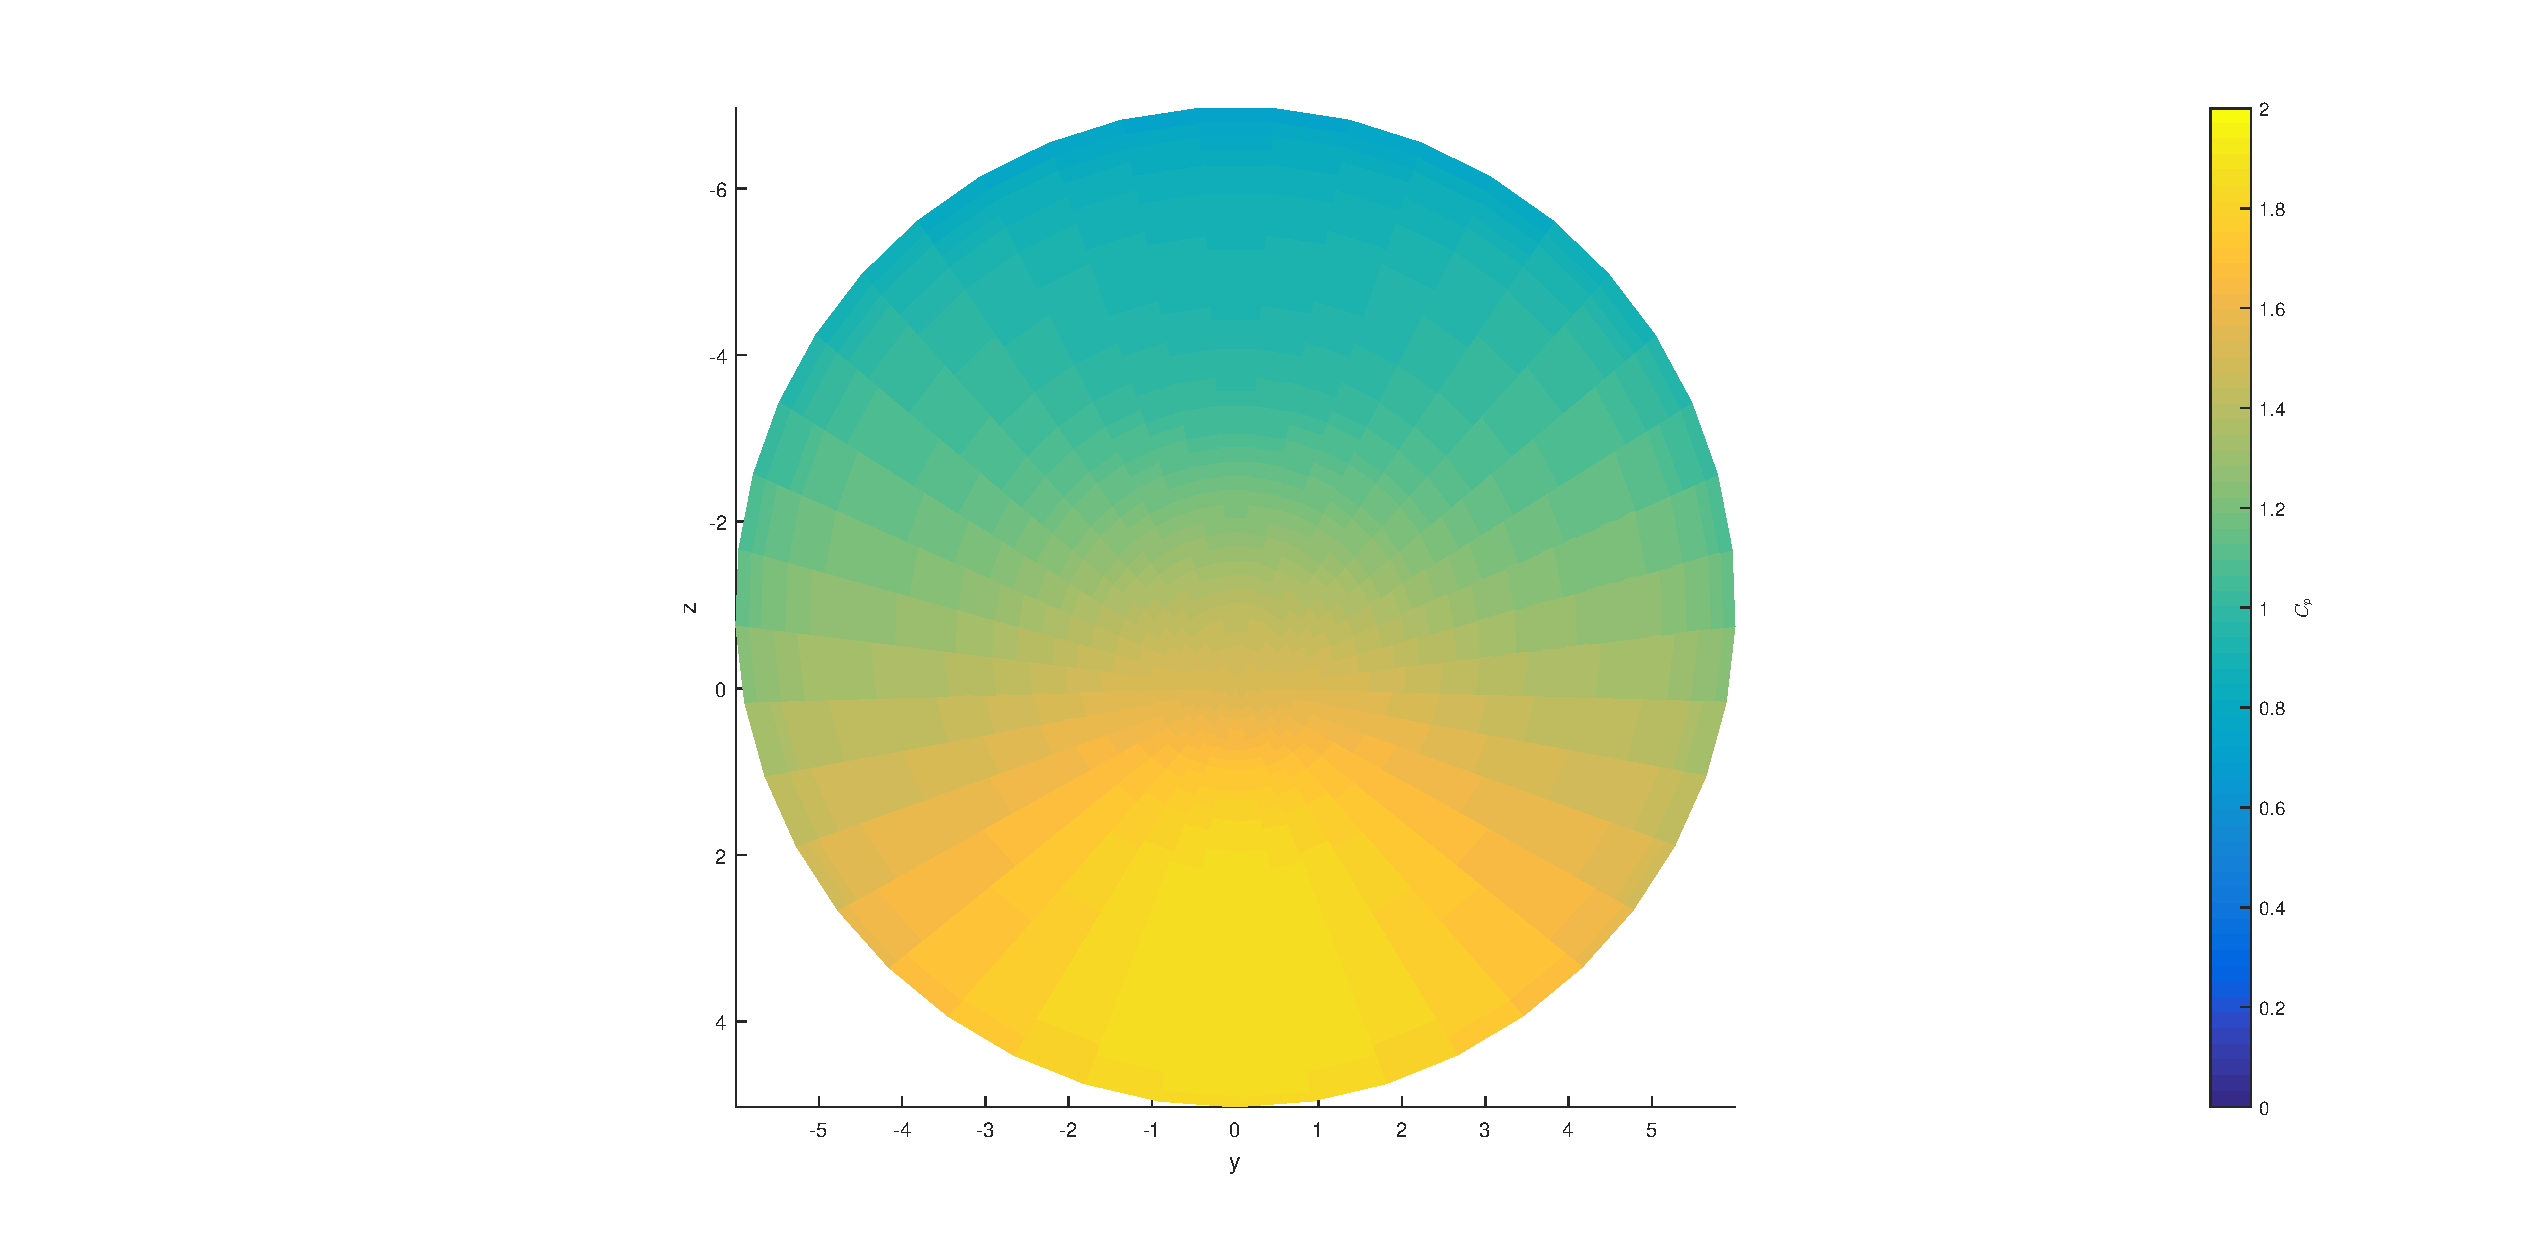
\includegraphics[width=1\textwidth]{./Figure/Structure/FrontviewCpDist}
\caption{Pressure distribution at the trimmed angle of attack} 
\label{fig:struc_pres}
\end{figure}

\subsubsection{Mass estimation method}

In order to verify that the mass estimation method described in Reference \cite{Samareh2011} has been correctly implemented, results for the nine sample cases presented on page 16 of Reference \cite{Samareh2011} have been checked. These nine sample cases were implemented by choosing the input parameters as given in tabular form (Tables 4 and 5) on page 16 of Reference \cite{Samareh2011} and the output parameters, primarily component masses and geometric quantities, were compared. A maximum error of 3 $\%$ in terms of total mass was obtained; a maximum error of 2 $\%$ in component masses. These errors are deemed sufficiently small to verify successful implementation of the mass estimation method.

Validation is performed indirectly: the method \cite{Samareh2011} has been applied in the \gls{edlsa} project \cite{Cianciolo2010}, where it was shown to yield results conforming well to the outcomes of a high-fidelity \gls{fem}. The used \gls{fem} is a validated tool \cite{Cianciolo2010} and thereby the method outlined in Reference \cite{Samareh2011} has been validated through comparison with a high-fidelity validated model. Moreover, the expression for minimum inflation pressure obtained by Samareh has been found to be in correspondence with Yamada et al \cite{Yamada2009}, Clark \cite{Clark2009} and Brown \cite{Brown2009}.







\subsection{Thermodynamics} \label{sec:VandVthermo}
\subsection{Thermodynamics in (re-)entry vehicles}\label{sec:thermo}
Thermodynamics is used for analysis such that components of the reentry vehicle stay within a certain temperature range. This allowed temperature range is a function of the intended use of the components and material selection. This literature review is broken down in three major parts. The first briefly explains the principles needed to describe the transfer of heat within structures. The second concerns the heat shield needed for the reentry phase, which is heavily linked to the aerodynamics. This is split up in non-inflatable and inflatable heat shields. The third deals with the thermal control of the capsule itself. The temperature inside the capsule should be suitable for human payload.

\subsubsection{Thermodynamic principles}
At the start of the mission the reentry vehicle can be seen as a closed system that has a total energy (\gls{sym:E}) in the form of internal energy (\gls{sym:U}), kinetic energy (\gls{sym:KE}) and potential energy (\gls{sym:PE}). For successful reentry the kinetic and potential are to be reduced. This can be done by transferring the energy across the boundary of the system. There are three methods to transfer the energy. Energy transfer by heat, by work and by mass flow. The latter requires the system to be open such that mass is allowed to leave the system \cite{Cengel2010}. An example of energy transfer by heat is the heating of gas near the wall of the heat shield and heating of the heat shield itself. Energy transfer by work could for example be the work done by the skin friction drag. The use of thrusters is an example of energy transfer due to mass flow as the propellant mass flows out of the open system. 

Energy transfer by heat, or simply heat transfer, has three modes: conduction, convection and radiation. Conduction is the transfer of heat between particles of a material due to interactions between these particles. Convection is the transfer of heat between a solid surface and a moving fluid. Radiation is transfer of heat due to the emission of electromagnetic energy from a surface to its surroundings \cite{Cengel2010, Karam1998}. Each of these modes can be described by governing equations as described in Ref.\cite{Holman2002}. Radiation is given by the Stefan-Boltzmann law and conduction by Fourier's law \cite{Cengel2010, Holman2002}.

\subsubsection{Thermal protection system}
The thermodynamic principles can be used to design a heat shield. The design of such a heat shield, also called a \acrfull{tps}, depends on several parameters. In general it all comes down to the trajectory the reentry vehicle will follow. The steeper the reentry trajectory, the larges the deceleration and the more g-loads will be endured by the (human) payload. The reentry vehicle will have a nominal trajectory with deviations. An overshoot results in a longer descent and can result in skipping off the planet, whereas an undershoot will result in a high descent rate. The larger the overshoot angle, the longer the reentry vehicle will be in atmosphere an thus creating a higher heat loading on the structure. On the other hand, for a larger undershoot angle, the heat development over time will be faster inducing a larger heat flux on the system. Also, the undershoot angle determines the trajectory with the highest dynamic pressure, which is important for structural sizing. 

Not only the trajectory is important for the design, but also the vehicle shape. The bigger the heat shield and the larger the bluntness, the more the thermal loads can be distributed over the capsule. This will result in a thinner \gls{tps} such that less mass is needed. This can cause aerodynamic instability, however \cite{Smoot}.

The temperature development in the structure through multiple layers of material can be determined when the heat loading and heat flux is known. An example of a method to determine the heat development is given by \cite{Hollis}.

\subsubsection*{Heat shield for non-inflatable structures}

Throughout the last century several reentry attempts have been performed with different \gls{tps}s. This paragraph focuses on several concepts for non-inflatable structures; the next paragraph on inflatables. 

A typical \gls{tps} example of a non-inflatable structure is the \gls{tps} of the reentry vehicle of the Apollo mission \cite{Pavlosky1974}. Different from inflatables, the \gls{tps} of the Apollo also has an aft shield and a crew compartment heat shield, because the front shield cannot deflect the direct flow from the sides and the aft part of the structure. An overview of the \gls{tps} lay-up is shown in figure \ref{fig:tpslayupapollo}. It consist of an ablative layer, which is sacrificed during reentry. The second layer is brazed stainless steel. This layer is followed by an insulator to keep the temperature difference between the outer layers and the inner layers. Last but not least, the connection to the rest of the structure is an aluminum honeycomb structure.

\begin{figure}[H]
\centering
\includegraphics[width = 0.55\textwidth]{Figure/tpsApollo.png}
\caption[Example of the Thermal Protection System lay-up for the Apollo reentry vehicle]{Example of the Thermal Protection System lay-up for the Apollo reentry vehicle \cite[p.5]{Pavlosky1974}.}
\label{fig:tpslayupapollo}
\end{figure}

\subsubsection*{Heat shield for inflatable structures}

The usage of  an inflatable structure is preferable over a non-inflatable structure for several reasons. An inflatable heat shell is not directly limited to the size of the launcher. Therefore a much larger diameter of the \gls{tps} can be obtained. This is an advantage because the heat loads on the structure can be distributed resulting in a lower front shell mass. Furthermore, the heat at the back side of the vehicle will be severely lower, such that there is no need for a back shell \cite{Hughes2005}. Therefore, less mass is needed and less effort needs to be done to verify and validate the thermal loads on payload closely located to the back shell. Although the system is very promising in terms of mass, the system does add a lot of complexity. 

The \gls{tps} of the IRVE vehicles consists of several layers \cite{Litton2011} which are shown in Figure \ref{fig:tpslayup}. The outer layer protects the structure from the direct incoming flow by distributing and absorbing or dissipating the heat. Also, it will carry the shearing loads from the flow. The second layer is an insulator and keeps the temperature behind the shield at a low level. Finally, the last Kevlar layer provides a fabric connection between the heat shield and the rest of the structure and carries most of the structural loads. The Kapton layers are impermeable and keep hot gases from passing the wall lay-up.

\begin{figure}[H]
\centering
\includegraphics[width = 0.55\textwidth]{Figure/IRVE4TPS.jpg}
\caption[Example of the \gls{tps} lay-up for the IRVE-4 reentry vehicle]{Example of the \gls{tps} lay-up for the IRVE-4 reentry vehicle\cite[p.6]{Litton2011}.}
\label{fig:tpslayup}
\end{figure}

There has not yet been an actual entry on Mars with an inflatable shield, but \gls{nasa} has demonstrated a well verified and validated concept \cite{Dillman2010, Dillman2012}. Another non-verified concept is the use of ballutes, which can be applied in case of high mass transportation \cite{Hall2001}. Due to its large size the thermal loads on the structure are small. However, the capsule, located in front of the ballute is exposed to a the free flow and needs additional thermal protection.

\subsubsection{Thermal control system}
For the \gls{tcs} of the crew capsule the book on Thermal Control by R. Karam is leading\cite{Karam1998}. Karam explains that heat fluxes due to conduction and radiation can be related to temperature using certain proportionality factors that depend on physical constants, material properties, surface conditions, geometry and temperature. The purpose of thermal control is to change the proportionality factors such that the desired temperature range is reached and retained. The changing of the proportionality factors is done by proper selection of materials and configurations.

The actual \gls{tcs} is divided into two parts, namely passive and active thermal control. The distinction is made whether the control component uses power or not. For example the use of insulation is a form of passive thermal control. Radiators and heaters are examples of active thermal control. Also a hot and cold case are considered to define the upper and lower limits for the temperatures. The hot case has the maximum possible influx of heat during the mission and the cold case the minimum possible influx of heat during the mission. Naturally these limits should lie within the desired temperature range. If this is not the case, the \gls{tcs} should be improved \cite{Karam1998}.

Karam also describes how to perform thermal analysis using thermal models, which can be used in combination with Holman's book on heat transfer \cite{Holman2002}. The predictions made in the thermal analysis rely on the law of conservation of energy. Both books (\cite{Karam1998,Holman2002}) describe how to do the analysis with computational methods, where Holman elaborates more on the use of a grid to find the thermal distributions at certain times. In this way the \gls{tcs} can be verified by analysis.







\end{document}